% !Mode:: "TeX:DE:UTF-8:Main"
%
%
%JOURNAL CODE  SEE DOCUMENTATION

\documentclass[examplefnt,biber]{../src/nowfnt} % creates the journal version, needs biber version
%wrapper for book and ebook are created automatically.

\usepackage[utf8]{inputenc}

\usepackage{amsmath,amssymb,amsfonts,latexsym,dsfont,xspace}

\usepackage{dirtytalk}
\usepackage{graphicx}
\usepackage{caption}
\usepackage{subcaption}
\usepackage{tikz-qtree}
% \usepackage{qtree}
% \usepackage{linguex}
% \newsavebox{\partbox}

\graphicspath{{../figures/}}

% a few definitions that are *not* needed in general:
\newcommand{\ie}{\emph{i.e.}}
\newcommand{\eg}{\emph{e.g.}}
\newcommand{\etc}{\emph{etc}}

% neural network functions
\newcommand{\ff}{\textsc{FeedForward}}
\newcommand{\rnn}{\textsc{Rnn}}
\newcommand{\lstm}{\textsc{Lstm}}
\newcommand{\rnng}{\textsc{Rnng}}
\newcommand{\birnn}{\textsc{BiRnn}}
\newcommand{\bilstm}{\textsc{BiLstm}}

% RNNG actions
\newcommand{\reduce}{\textsc{reduce}}
\newcommand{\open}{\textsc{open}}
\newcommand{\shift}{\textsc{shift}}
\newcommand{\gen}{\textsc{gen}}
\newcommand{\discactions}{A_{\mathcal{D}}}
\newcommand{\genactions}{A_{\mathcal{G}}}


% blocking gradient in computation graph
\newcommand{\blockgrad}{\textsc{BlockGrad}}

% probability models
\newcommand{\ptheta}{p_{\theta}}  % sentence
\newcommand{\qlambda}{q_{\lambda}}  % sentence

%% math symbols
\newcommand{\reals}{\ensuremath{\mathbf{R}}}  % real numbers
\newcommand{\dataset}{\ensuremath{\mathcal{D}}}  % dataset

\newcommand{\defeq}{\ensuremath{\triangleq}}  % define something with an equation

\newcommand{\x}{\ensuremath{\mathbf{x}}}  % sentence
\newcommand{\y}{\ensuremath{\mathbf{y}}}  % tree
\newcommand{\h}{\ensuremath{\mathbf{h}}}  % hidden vector
\newcommand{\fw}{\ensuremath{\mathbf{f}}}  % forward lstm feature
\newcommand{\bw}{\ensuremath{\mathbf{b}}}  % backward lstm feature

\newcommand{\veca}{\ensuremath{\mathbf{a}}}
\newcommand{\vecb}{\ensuremath{\mathbf{b}}}
\newcommand{\vecr}{\ensuremath{\mathbf{r}}}
\newcommand{\vecs}{\ensuremath{\mathbf{s}}}
\newcommand{\vecu}{\ensuremath{\mathbf{u}}}
\newcommand{\vecv}{\ensuremath{\mathbf{v}}}
\newcommand{\vecw}{\ensuremath{\mathbf{w}}}

\newcommand{\vecR}{\ensuremath{\mathbf{R}}}
\newcommand{\vecS}{\ensuremath{\mathbf{S}}}
\newcommand{\vecV}{\ensuremath{\mathbf{V}}}
\newcommand{\vecW}{\ensuremath{\mathbf{W}}}


\DeclareMathOperator{\indicator}{\mathbf{1}}  % indicator function

% \DeclareMathOperator{\expect}{E} % expectation
% \DeclareMathOperator{\expect}{\rm I\kern-.3em E} % expectation (thicker letter)
\DeclareMathOperator{\expect}{\mathbf{E}} % expectation
\DeclareMathOperator{\var}{\mathbf{var}} % variance
\DeclareMathOperator{\cov}{\mathbf{cov}} % covariance
\DeclareMathOperator{\corr}{\mathbf{corr}} % covariance

\DeclareMathOperator{\objective}{\mathcal{L}}  % objective function
\DeclareMathOperator{\elbo}{\mathcal{E}}  % elbo objective
\DeclareMathOperator{\yieldx}{\mathcal{Y}(\x)}  % yield of a sentence x

\DeclareMathOperator{\rev}{\text{reverse}}  % reverse a sequeunce
\DeclareMathOperator{\concat}{\circ}  % concatenate vectors


%ARTICLE TITLE
\title{Latent syntax in a deep generative model of language}


%ARTICLE SUB-TITLE
% \subtitle{Language models with latent syntactic structure}


%AUTHORS FOR COVER PAGE
% separate authors by \and, item by \\
% Don't use verbatim or problematic symbols.
% _ in mail address should be entered as \_
% Pay attention to large mail-addresses ...

%if there are many author twocolumn mode can be activated.
%\booltrue{authortwocolumn} %SEE DOCUMENTATION
\maintitleauthorlist{
  Daan van Stigt \\
  Institute for Logic, Language and Computation \\
}

%BIBLIOGRAPHY FILE
\addbibresource{../src/bibliography.bib}

\begin{document}

\makeabstracttitle

\begin{abstract}
In this thesis I investigate the question: \textit{What are effective ways of incorporating syntactic structure into neural language models?}

In this thesis I:
\begin{itemize}
  \item study a class of neural language models that merges generative transition-based parsing with recurrent neural networks in order to model sentences together with their latent syntactic structure;
  \item propose a new globally trained chart-based parser as an alternative proposal distribution used in the approximate marginalization;
  \item propose effective methods for semisupervised learning, making the syntactic structure a latent variable;
  \item perform targeted syntactic evaluation and compare the model's performance with that of alternative models that are based on multitask learning.
\end{itemize}
I find that:
\begin{itemize}
  \item ...
  \item ...
\end{itemize}
\end{abstract}

% end of main matter
\begin{acknowledgements}
First and foremost I want to thank my mother, who paid for my studies and washed my black hoodie every once in a while. Next want to thank Adventure Time for fending off depression during the writing of this work. And thank you Wilker for keeping it real. Thank you, next.
\end{acknowledgements}


\chapter{Introduction}
\label{01-introduction}
% \bibliography{../src/bibliography}

This thesis investigates the question: \textit{What are effective ways of incorporating syntactic structure into neural language models?}

We study a class of neural language models that explicitly model the hierarchical syntactic structure in addition to the sequence of words \citep{Dyer+2016:RNNG,Buys+2015:neural-gen-dep,Buys+2018}. These models merges generative transition-based parsing with recurrent neural networks in order to model sentences together with their latent syntactic structure. The syntactic structure that decorates the words can be latent, and marginalized over, or can be given explicitly, for example as the prediction of an external parser. Although these are fundamentally joint model, they can be evaluated as regular language models (modeling only words) by (approximate) marginalization of the syntactic structure. In the case of the RNNG \citep{Dyer+2016:RNNG}, exact marginalization is intractable due to the parametrization of the statistical model, but importance sampling provides an effective approximate method. An externally trained discriminative parser is used to obtain proposal samples. Other models provide exact marginalization, but this typically comes at the cost of a less expressive parametrization, for example one in which the features cannot be structure-dependent \citep{Buys+2018}.

In this thesis I study the RNNG \citep{Dyer+2016:RNNG} and investigate:

\paragraph{The approximate marginalization} I propose an alternative proposal distribution and investigate the impact.
\begin{itemize}
  \item I propose a new discriminative chart-based neural parser that is trained with a global, Conditional Random Field (CRF), objective. The parser is an adaptation of the minimal neural parser proposed in \citet{stern2017minimal}, which is trained with a margin-based objective.
  \item This contrast with the choise of \citet{Dyer+2016:RNNG} for a transition-based parser as proposal, a discrminatively trained RNNG.
  \item We posit that a globally trained model is a better proposal distribution than a locally trained transition based model: a global model has ready access to competing analyses that can be structurally dissimilar but close in probability, whereas we hypothesize that a locally trained model is prone to produce locally corrupted structures that are nearby in transition-space.
  \item In a transition based parser more diverse samples can be obtained by flattening the transition distributions. This causes the model to be less confident in its predictions. A downside is that this approach causes the model to explore parts of the probability space which it has not encountered during training.
  \item The above is a general challenge for greedy transition based models that can be answered to by training with dynamic oracles \citep{Goldberg+2013:dynamic}, also called `exploration' (\citep{Ballesteros+2016:exploration,stern2017minimal}. These approaches can be considered instances of imitation learning \citep{Vlachos2012:imitation,Eisner+2012:imitation}.
  \item We do not consider these directions in this thesic. Dynamic oracles can produce substantial improvements in constituency parsing performance, but they must be custom designed for each transition system \citep{Klein+2018:reinforce}.
\end{itemize}


\paragraph{Semi-supervised training by including unlabeled data} To make joint models competitive language models they need to make use of the vast amounts of unlabeled data that exists.
\begin{itemize}
  \item A major drawback of these syntactic language models is that they require annotated data to be trained, and preciously little of such data exists.
  \item We extend the training to the unsupervised domain by optimizing a variational lower bound on the marginal probabilities that jointly optimizes the parameters of proposal model ('posterior' in this framework) with the joint model.
  \item We obtain gradients for this objective using the score function estimator \citep{Fu2006}, also known as REINFORCE \citep{Williams1992:REINFORCE}, which is widely used in the field of deep reinforcement learning, and we introduce an effective baseline based on argmax decoding \citep{Rennie+2017:argmax-baseline}, which significantly reduces the variance in this optimization procedure.
  \item Our CRF parser particularly excels in the role of posterior thanks the independence assumptions that allow for efficient exact computation of key quantities: the entropy term in the lower bound can be computed exactly using Inside-Outside algorithm, removing one source of variance from the gradient estimation, and the argmax decoding can be performed exactly thanks to Viterbi, making the argmax baseline even more effective.
\end{itemize}

\paragraph{Alternative, simpler, models} There are alternatives to the methods that this thesis investigates.
\begin{itemize}
  \item Multitask learning of a neural language model with a syntactic side objective is a competitive and robust alternative method to infuse neural language models with syntactic knowledge.
  \item Training the syntactic model on data that mixes gold trees with predicted `silver' trees for unlabeled data is a competitive and robust alternative to fully principled semi-supervised learning.
  \item We propose a simple multitask neural language model that predicts labeled spans from the RNN hidden states, using a feature function identical identical to that used in the CRF parser. A similar strategy has recently proposed in work on semantic parsing and is called a `syntactic scaffold' \citep{Swayamdipta+2018:scaffold}.
  \item We consider these alternatives in order to quantify significance of the latent structure and the semisupervised training as measured by some external performance metric.
\end{itemize}

\paragraph{Targeted syntactic evaluation}
TBA



\chapter{Background}
\label{02-background}
This section provides background on the four topics that are combined in this thesis: syntax, parsing, language modelling, and neural networks.

\section{Syntax}
We first introduce some concepts relating to syntax that are relevant for this thesis. In particular, we introduce the notion of a \textit{constituent}, and the hierarchical organization of constituents in a sentence as described by phrase-structure grammars. The aim is to provide a succinct and compelling answer to the question: \textit{Why should we care about constituency structure when modelling language?}

The exposition primarily follows \citet{huddleston2002grammar}, a well established reference grammar of the English language that is relatively agnostic with respect to theoretical framework, with some excursions into \citet{carnie2010constituent} and \citet{everaert2015structures}, which are less language-specific but rooted more in a particular theoretical framework\footnote{Broadly subsumable under the name \textit{generative grammar}.}.

We take the following three principles from \citet{huddleston2002grammar} as guiding:
\begin{enumerate}[noitemsep]
  \item \textit{Sentences consist of parts that may themselves have parts.}
  \item \textit{These parts belong to a limited range of types.}
  \item \textit{The constituents have specific roles in the larger parts they belong to.}
\end{enumerate}
To each principle we now dedicate a separate section.

\subsection{Constituents}
Sentences consist of parts that may themselves have parts. The parts are groups of words that function as units and are called \textit{constituents}. Consider the simple sentence \textit{A bird hit the car.} The immediate constituents are \textit{a bird} (the subject) and \textit{hit the car} (the predicate). The phrase \textit{hit the car} can be analyzed further as containing the constituent \textit{the car}. The ultimate constituents of a sentence are the atomic words, and the entire analysis is called the constituent structure of the sentence. This structure can be indicated succinctly with the use of brackets
\exi. [ [ A bird ] [ hit [ the car ] ] ]

or less succinctly as a tree diagram.
\begin{figure}[h]
  \center
  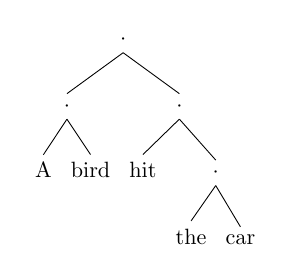
\begin{tikzpicture}[scale=.8]
    \Tree [.$\cdot$ [.$\cdot$ A bird ] [.$\cdot$ hit [.$\cdot$ the car ] ] ]
  \end{tikzpicture}
  \label{fig:bird-tree}
\end{figure}
Evidence for the existence of such constituents can be provided by examples such as the following, which are called constituent tests \citep{carnie2010constituent}. Consider inserting the adverb \textit{apparently} into our example sentence, to indicate the alleged status of the event described in the sentence. In principle there are six positions available for the placement of \textit{apparently} (including before, and after the sentence). However, only three of these placements are actually permissible:\footnote{We use an asterisk * to indicate a sentence that is judged ungrammatical, as is customary in linguistics.}
\exi.\a. \textit{Apparently} a bird hit the car.
  \b. *An \textit{apparently} bird hit the car.
  \c. A bird \textit{apparently} hit the car.
  \d. *A bird hit \textit{apparently} the car.
  \e. *A bird hit the \textit{apparently} car.
  \f. A bird hit the car, \textit{apparently}.

Based on the bracketing that we proposed for this sentence we can formulate a general constraint: the adverb must not interrupt any constituent. Indeed, this would explain why \textit{apparently} cannot be placed anywhere inside \textit{hit the car} and not between \textit{a} and \textit{bird}. For full support, typically, results from many more such test are gathered, and in general these tests can be much more controversial than in our simple example \citep{carnie2010constituent}.

\subsection{Categories}
The constituents of a sentence belong to a limited range of types that form the set of syntactic categories. Two types of categories are distinguished: lexical and phrasal. The lexical categories are also known as part-of-speech tags. A tree can be represented in more detail by adding lexical (D, N, V) and phrasal categories (S, NP, VP).
\begin{figure}[h]
  \center
  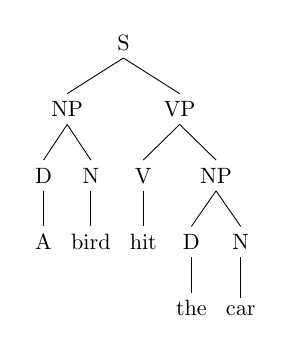
\begin{tikzpicture}[scale=.8]
    \Tree [.S [.NP [.D A ] [.N bird ]] [.VP [.V hit ] [.NP [.D the ] [.N car ] ] ] ]
  \end{tikzpicture}
\end{figure}
In this example, the noun (N) \textit{car} is the head of the noun phrase (NP) \textit{the car}, while the head of the larger phrase \textit{hit the car} is the verb (V) \textit{hit}, making this larger constituent a \textit{verb phrase} (VP). The whole combined forms a sentence (S).

\subsection{Hierarchy}
The constituents have specific roles in the larger parts they belong to. This structure provides constraints that are not explainable from the linear order of the words themselves \citep{everaert2015structures}. Consider for instance the following example of the syntactic behaviour of \textit{negative polarity items} (NPIs) from \citet{everaert2015structures}. A negative polarity item is, to first approximation, a word or group of words that is restricted to negative context \citep{everaert2015structures}.\footnote{More generaly, they are words that need to be licensed by a specific \textit{licencing context} \citep{giannakidou2011npi}.} Take the behaviour of the word \textit{anybody}:
\exi.\a. The talk I gave did \textit{not} appeal to \textit{anybody}.
     \b. *The talk I gave appealed to \textit{anybody}.
     \c. *The talk I did \textit{not} give appealed to \textit{anybody}.

From sentences (a) and (b) we might formulate the hypothesis that the word \textit{not} must linearly precede the word \textit{anybody}, but a counter example refutes this hypothesis: sentence (c) is also not grammatical. Instead---it is argued---the constraints that govern this particular pattern depend on hierarchical structure: the word \textit{not} must `structurally precede' the word \textit{anybody} \citep{everaert2015structures}. Figure \label{ref:trees-npi} shows the constituent structure of both sentences. The explanation goes as follows: \say{In [the left tree] the hierarchical structure dominating \textit{not} also immediately dominates the hierarchical structure containing \textit{anybody}. In [the right tree], by contrast, \textit{not} sequentially precedes \textit{anybody}, but the triangle dominating \textit{not} fails to also dominate the structure containing \textit{anybody}.} \citep{everaert2015structures}.

\begin{figure}[h]
  \center
  \begin{subfigure}[b]{0.5\textwidth}
		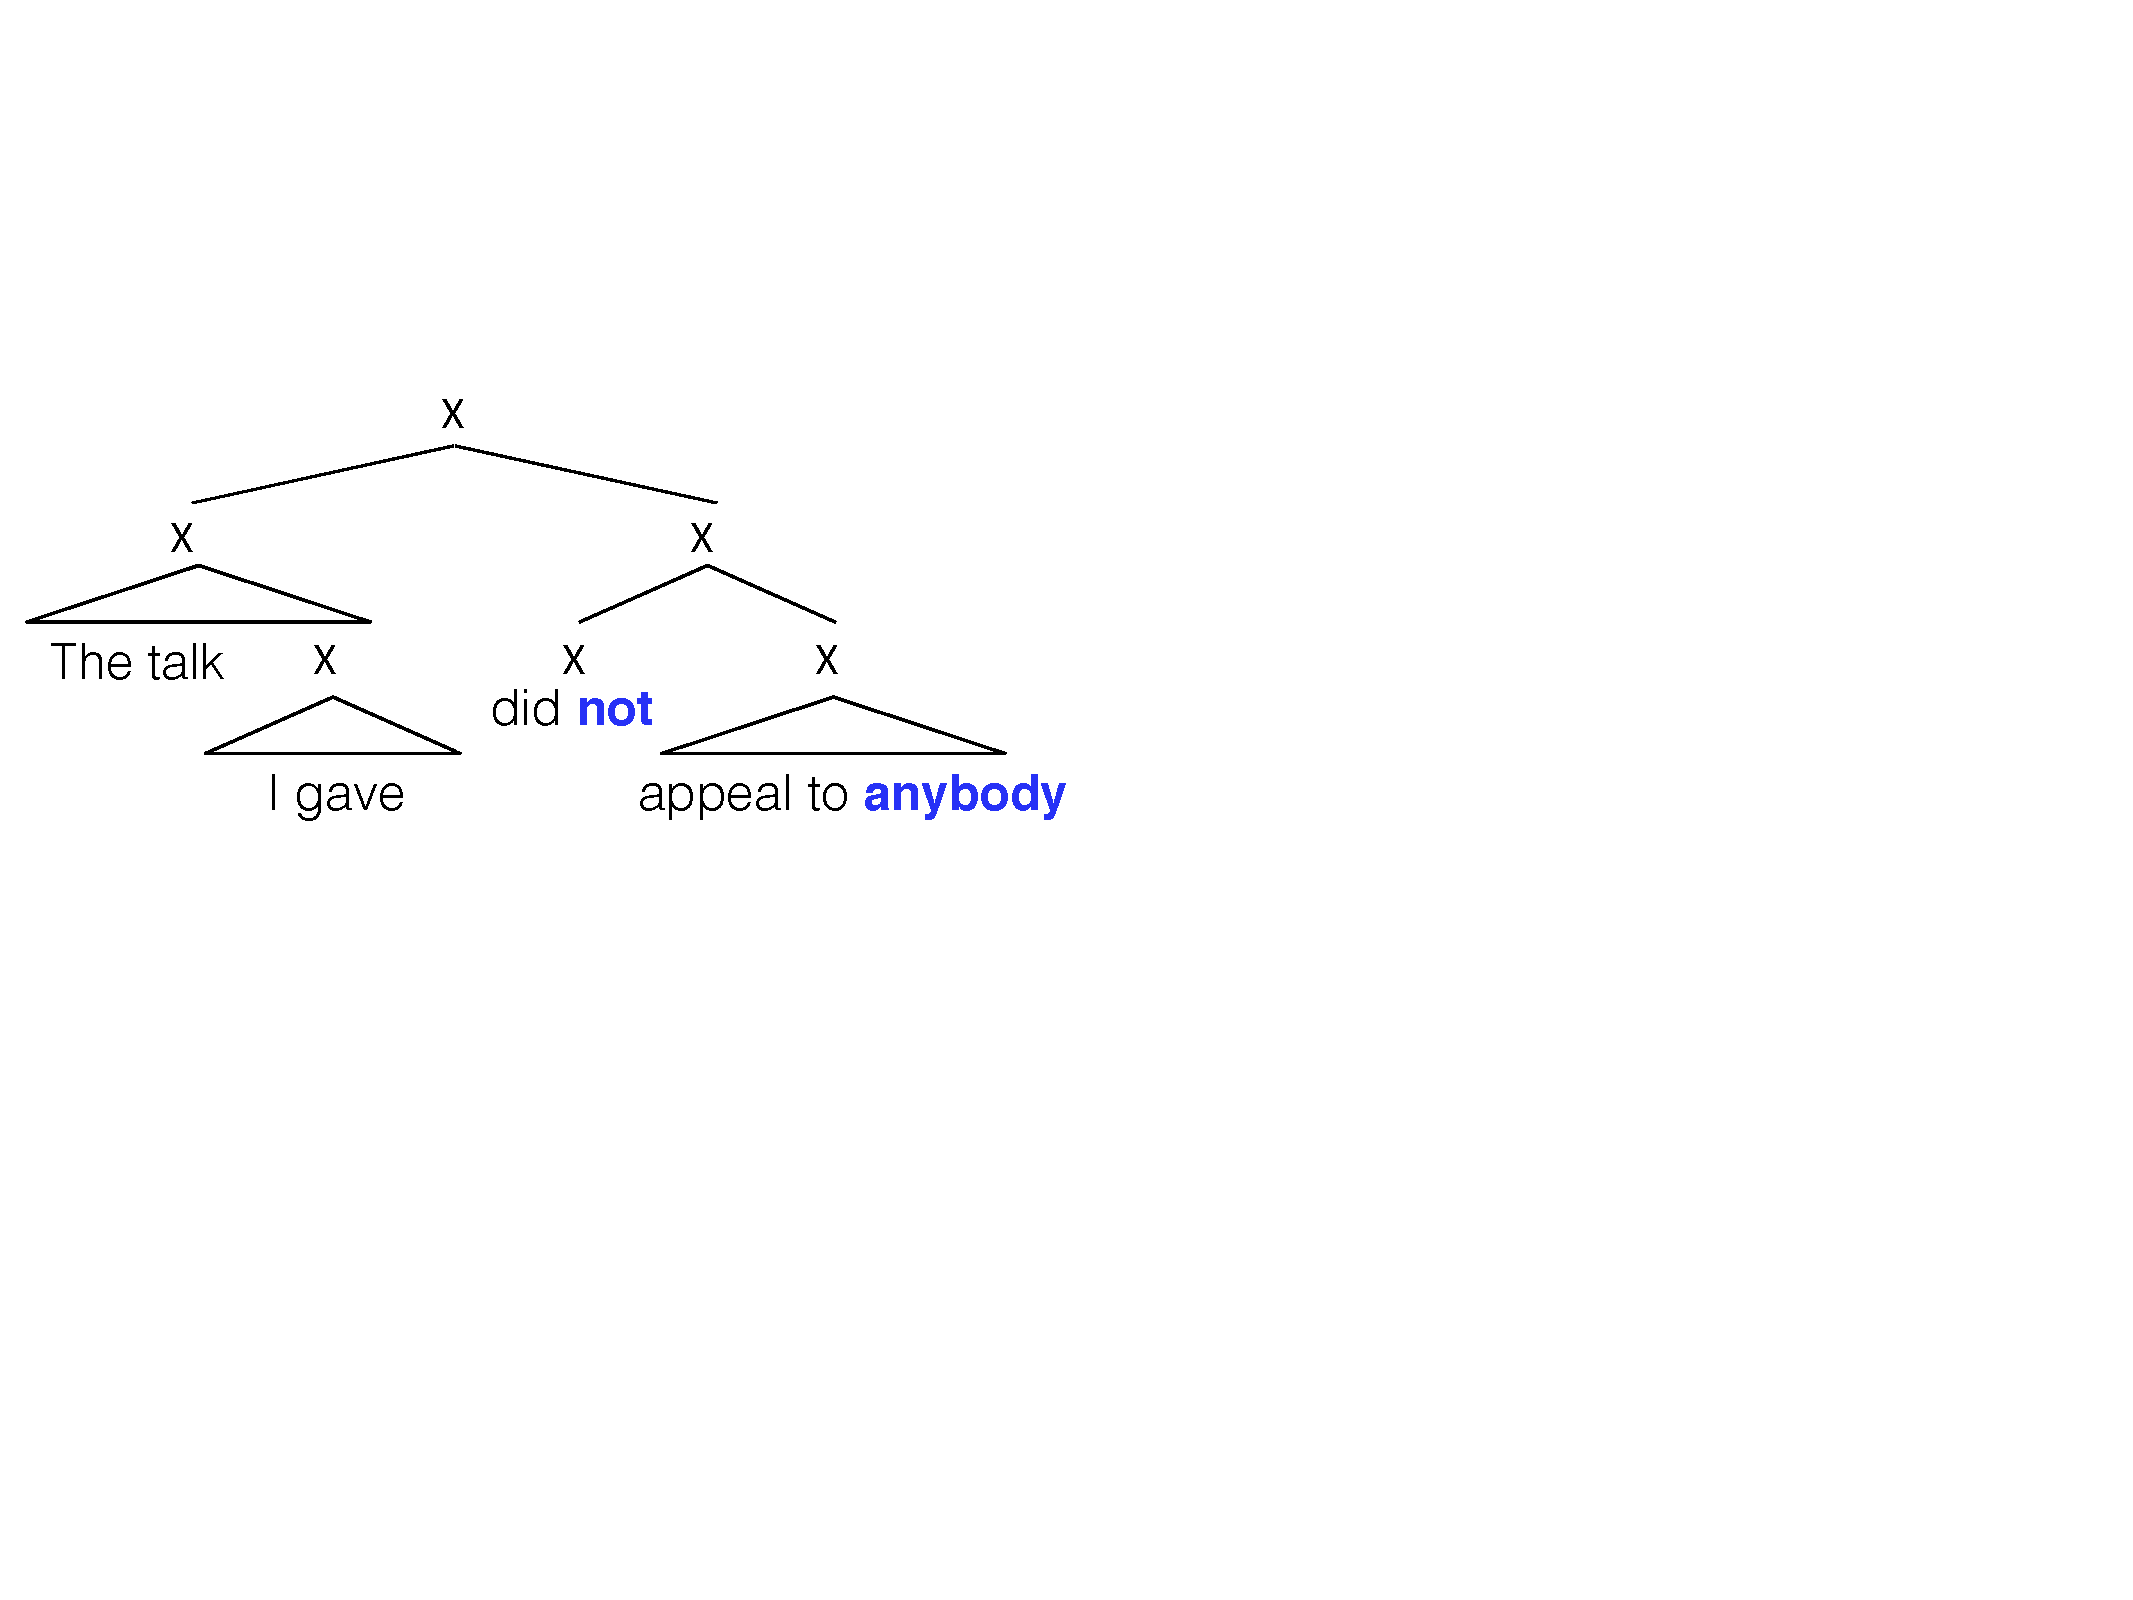
\includegraphics[width=\textwidth]{trees/npi-licensed.pdf}
	\end{subfigure}
	\begin{subfigure}[b]{0.45\textwidth}
		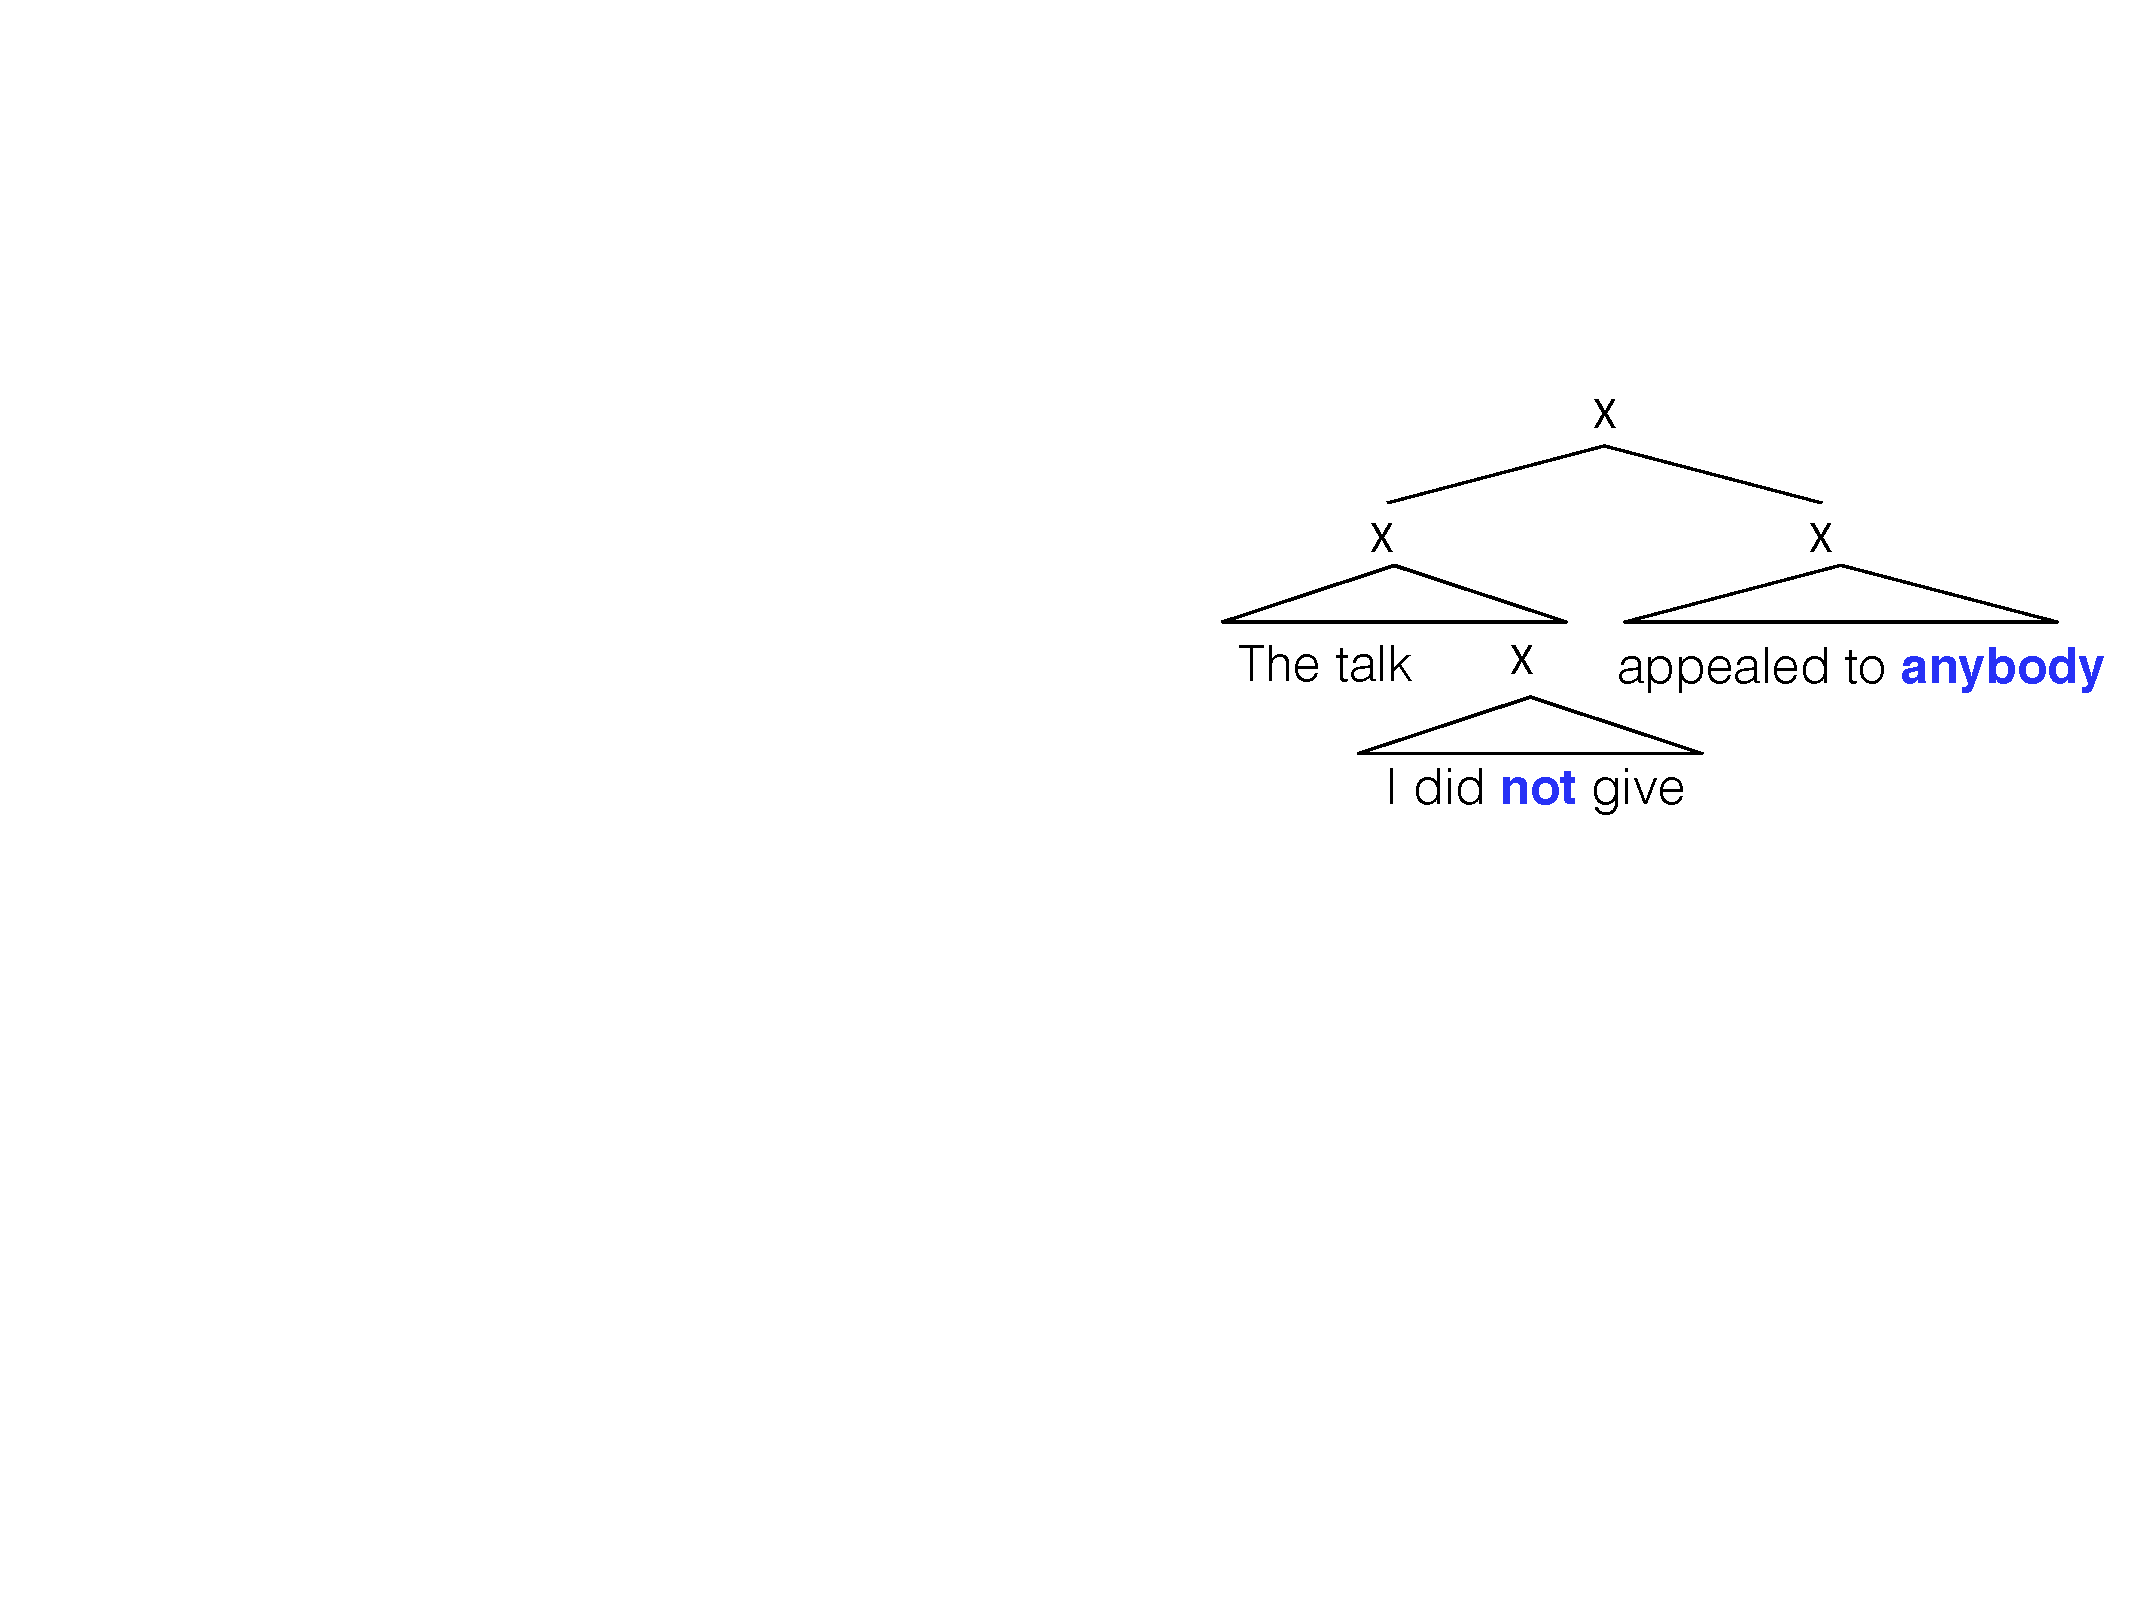
\includegraphics[width=\textwidth]{trees/npi-unlicensed.pdf}
	\end{subfigure}
\caption{Dependance on hierarchical structure of negative polarity items. Left shows the word \textit{anybody} in the licensing context of \textit{not}. Right shows the ungrammatical sentence where the word is not. Figure taken from \cite{everaert2015structures}. The triangles indicate substructre that is not further explicated.}
\label{fig:trees-npi}
\end{figure}


\subsection{Controversy}
Theoretical syntax is rife with controversy, and wildly differing viewpoints exist. In fact, for each point made in our short discussion the exact opposite point has been made as well:

\begin{itemize}
  \item Work in dependency grammar and other word-based grammar formalisms departs from the idea that lexical relations between individual words are more fundamental than constituents and their hierarchical organization \citep{tesniere1959elements,nivre2005dependency,hudson2010introduction}, and dispenses with the notion of constituents altogether.

  \item A recurring cause of controversy is the question whether hierarchical structure needs to be invoked in linguistic explanation. That is, whether the kind of analysis we presented with embedded, hierarchically organized constituents is really fundamental to language. \citet{frank2012hierarchical} argue for instance that a shallow analysis of sentences into immediate constituents with linear order but no hierachical structure\footnote{A structure reminiscent of that predicted in the task of \textit{chunking}, or shallow parsing.} is sufficient for syntactic theories, a claim that is vehemently rejected by \citet{everaert2015structures}.

  \item Research in cognitive neuroscience and psycholinguistics shows that human sentence processing is hierachical, giving evidence that processing crucially depends on the kind of structures introduced in the sections above \citep{hale2001earley,levy2008expectation,brennan2016abstract}. However, research also exists that shows that purely linear predictors are sufficient for modeling sentence comprehension, thus showing the exact opposite to be true \citep{conway2008neurocognitive,gillespie2011hierarchy,christiansen2012similar,gillespie2013against,frank2012hierarchical}.
\end{itemize}
Our work, however, takes a pragmatic position with respect to such questions: syntax, we assume, is whatever our dataset says it is. And to some degree, the question whether language is hierachical or linear is a question that this thesis engages with from a statistical and computational standpoint.

\section{Parsing}
  Parsing is the task of predicting a tree $\y$ for a sentence $\x$. Probabilitic parsers solve this problem by learning a probabilistic model $p$ that describes a probability distribution over \textit{all} the possible parses $\y$ of a sentence $\x$. This distribution quantifies the uncertainty over the syntactic analyses of the sentence, and can be used to make predictions by finding the trees with highest probability. A further benefit of the probabilistic formulation is that the uncertainty over the parses can be determined quantitatively by computing the entropy of the distribution, and qualitatively by obtaining samples from the distribution. This section describes the form that such probabilistic models take, and the data from which they are estimated.

  \begin{figure}[ht]

    \begin{subfigure}[b]{\textwidth}
      \center
      \begin{tikzpicture}[scale=.6]
        \Tree [.S
        [.SBAR-NOM-SBJ
          [.WHNP-1 What ]
          [.S [.NP-SBJ *T*-1 ] [.VP happened [.NP-TMP Friday ] ] ] ]
        [.VP
          was
          [.NP-PRD [.NP the worst ] [.PP of [.NP all worlds ] ] ] ]
        . ]

      \end{tikzpicture}
      \subcaption{Original Penn Treebank tree.}
      \label{fig:tree-original}
    \end{subfigure}

    \begin{subfigure}[b]{\textwidth}
      \center
      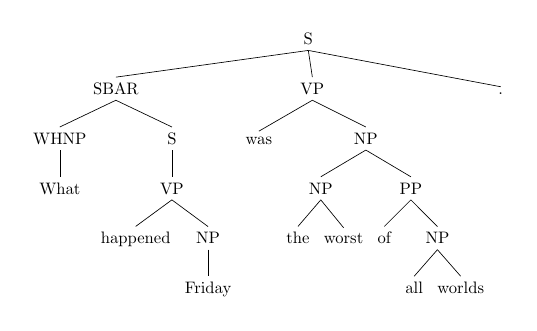
\begin{tikzpicture}[scale=.6]
        \Tree [.S
        [.SBAR [.WHNP What ] [.S [.VP happened [.NP Friday ] ] ] ]
        [.VP
          was
          [.NP [.NP the worst ] [.PP of [.NP all worlds ] ] ] ]
        $.$ ]

      \end{tikzpicture}
      \tiny
      \subcaption{Function tags and traces removed.}
      \label{fig:tree-simplified}
    \end{subfigure}

    \begin{subfigure}[b]{\textwidth}
      \center
      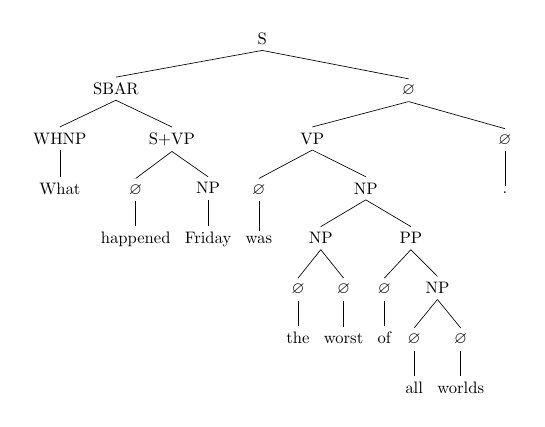
\begin{tikzpicture}[scale=.6]
        \Tree [.S
        [.SBAR [.WHNP What ] [.S+VP [.$\varnothing$ happened ] [.NP Friday ] ] ]
        [.$\varnothing$
          [.VP
            [.$\varnothing$ was ]
            [.NP
              [.NP [.$\varnothing$ the ] [.$\varnothing$ worst ] ]
              [.PP [.$\varnothing$ of ] [.NP [.$\varnothing$ all ] [.$\varnothing$ worlds ] ] ] ] ]
          [.$\varnothing$ . ] ] ]

      \end{tikzpicture}
      \tiny
      \subcaption{Converted to normal form using a dummy label $\varnothing$.}
      \label{fig:tree-cnf}
    \end{subfigure}

    \begin{subfigure}[b]{\textwidth}
      \center
      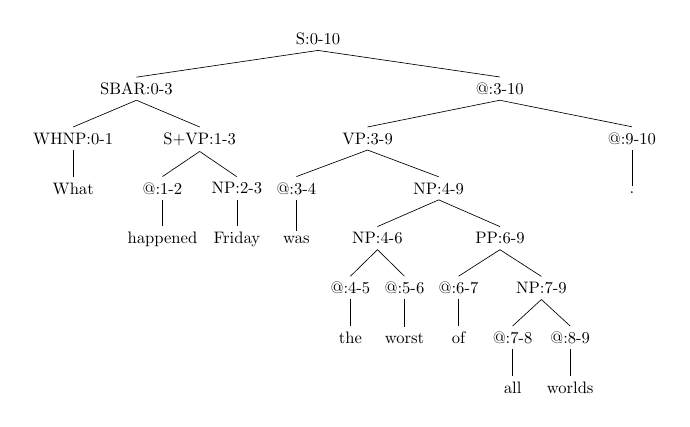
\begin{tikzpicture}[scale=.6]
        \Tree [.S:0-10
        [.SBAR:0-3
          [.WHNP:0-1 What ]
          [.S+VP:1-3 [.@:1-2 happened ] [.NP:2-3 Friday ] ] ]
        [.@:3-10
          [.VP:3-9
            [.@:3-4 was ]
            [.NP:4-9
              [.NP:4-6 [.@:4-5 the ] [.@:5-6 worst ] ]
              [.PP:6-9
                [.@:6-7 of ]
                [.NP:7-9 [.@:7-8 all ] [.@:8-9 worlds ] ] ] ] ]
          [.@:9-10 . ] ] ]

      \end{tikzpicture}
      \tiny
      \subcaption{In normal form with spans.}
      \label{fig:tree-cnf-spans}
    \end{subfigure}

  \caption{Converting a treebank tree (withouth part-of-speech tags).}
  \label{fig:trees-ptb}
  \end{figure}

  \subsection{Treebank}
    A treebank is a collection of sentences annotated with their grammatical structure that allows the estimation of statistical parsings models. The Penn Treebank \citep{marcus1993penn} is such a collection, consisting of sentences annotated with their constituency structure. Figure \ref{fig:tree-original} shows an example tree from this dataset and figure \ref{fig:tree-simplified} shows the tree after basic processing\footnote{This removes the functional tags and annotation of argument structure introduced in version 2 of the Penn Treebank \citep{marcus1994annotating}.}. Some of the models in this work require trees to be in \textit{normal form}: fully binary, but with unary branches at the terminals. Figure \ref{fig:tree-cnf} show the result of this (invertible) normalization, that is obtained by introduction of an empty dummy label $\varnothing$. Annotating the labels with left and right endpoints of the words they span results in the tree in figure \ref{fig:tree-cnf-spans}.

    A tree can be factorized into its parts: we can think of tree as a set of \textit{labeled spans}, or as a set of \textit{anchored rules}. A labeled span is a triple $(A, i, j)$ of a syntactic label $A$ from a labelset $\Lambda$ together with the left and right endpoints $i$, $j$ that the label spans. An \textit{anchored rule} is a triple $(r, i, j)$ or four-tuple $(r, i, k, j)$, containing a rule $r$ in normal form with span endpoints $i$, $j$, and a split-point $k$ of the left and right child when $r$ is not a lexical rule. Consider these two representations of the tree in figure \ref{fig:tree-cnf-spans} given in table \ref{tab:spans-rules}. These different factorizations will become relevant in chapter \ref{04-crf} when formulating the probabilistic model.

    \begin{table}[h]
      \center
      \small
      \bgroup  % increase vertical space
      \def\arraystretch{1.5}  % increase vertical space
      \begin{tabular}{l|l}
        Labeled spans & Anchored rules \\
        \hline
        (S, 0, 10)     & (S $\to$ SBAR $\varnothing$, 0, 3, 10)  \\
        (SBAR, 0, 3)   & (SBAR $\to$ WHNP S+VP, 0, 1, 3)  \\
        (WHNP, 0, 1)     & (WHNP $\to$ \textit{What}, 0, 1)  \\
        $\qquad\vdots$ & $\qquad\vdots$  \\
        ($\varnothing$, 9, 10)     & ($\varnothing$ $\to$ ., 9, 10)  \\
      \end{tabular}
      \caption{Two representations of the tree in \ref{fig:tree-cnf-spans}.}
      \label{tab:spans-rules}
      \egroup  % increase vertical space
    \end{table}


  \subsection{Models}
    The probabilistic model of a parser can be \textit{discriminative}, describing the conditional probability distribution $p(\y \mid \x)$, or \textit{generative}, describing the joint distribution $p(\x, \y)$. The form that the model takes is largely dictated by the algorithm used to build the parses.

    Transition-based methods formulate parsing as a sequence of shift-reduce decisions made by a push-down automaton that incrementally builds a tree. The design of the transition system determines whether the tree is constructed bottom-up, top-down,\footnote{Post-order and pre-order, respectively.} or otherwise, and determines whether the trees need to be in normal form. The probabilistic model is defined over the sequences of actions, and the probability distribution typically factorizes as the product of conditional distributions over the next action given the previous actions. This makes it a directed model that is \textit{locally normalized}.\footnote{With the exception of those approaches that instead define a Conditional Random Field over the action sequences \citep{andor2016globally}, in which case the model is defined over the globally normalized action sequences.}
    \begin{definition}{}
      A probalistic model $p$ over sequences $a \in \mathcal{A}^n$ is \textit{locally normalized} if
      \begin{align*}
        p(a)
          &= \prod_{i=1}^{n} p(a_i \mid a_{<i})  \\
          &= \prod_{i=1}^{n} \frac{ \Psi( a_{<i}, a_{i} ) }{ Z( a_{<i} ) },
      \end{align*}
      where $Z( a_{<i} ) = \sum_{a \in \mathcal{A}} \Psi( a_{<i}, a )$  is a local normalizer and $\Psi$ is a nonnegative scoring function: $\Psi( a_{<i}, a_{i} ) \geq 0$ for all $a_{<i}$ and $a$.
    \end{definition}
    Such a model is discriminative when the actions only build the tree, but can be made generative when word prediction is included in the action set.

    Chart based parsing, on the other hand, factorizes trees along their parts, and defines the probabilistic model over the shared substructures. Representing the model as the product of local parts greatly reduces the number of variables required to specify the full distribution, and allows the use of dynamic programming for efficient inference. Discriminitive models based on Conditional Random Fields (CRF) \citep{lafferty2001crf} follow this factorization: local functions independently predict scores for the parts, and the product of this score is normalized \textit{globally} by a normalizer that sums over the exponential number structures composable from the parts.
    \begin{definition}{}
      A probalistic model $p$ over sequences $a \in \mathcal{A}^n$ is \textit{globally normalized} if
      \begin{align*}
        p(a) = \frac{ \Psi( a ) }{ Z },
      \end{align*}
      where $Z  = \sum_{a \in \mathcal{A}^n} \Psi( a )$ is a \textit{global} normalization term, and $\Psi( a ) \geq 0$ for all $a$. To allow efficient computation of the normalizer $Z$, the function $\Psi$ typically factors over parts of $a$ as $\Psi ( a ) = \prod_{i=1}^K \psi (a_i )$ with the choice of parts $a = \{a_i\}_{i=1}^K$ depending on the model.
    \end{definition}
    Generative chart-based models, instead, estimate rule probabilities directly from a treebank. The probability of a tree is computed directly as the product of the probabilities of the rules that generate it, thus requiring no normalization.\footnote{In fact, this makes generative chart-based models directed, locally normalized models: they generate trees top-down by expanding localized normally rules.}.

    Either method have their advantages and disadvantages. The transition-based methods are fast, running in time linear in the sequence length, and allow arbitrary features that can condition on the entire sentence and the partially constructed derrivation. However, directed models with local normalization are known to suffer from the problem of label bias \citep{lafferty2001crf}, and conditioning on large parts of the partial derivations prohibits exact inference, so that decoding can be done only approximately, either with greedy decoding or with beam search. The chart based methods, on the other hand, allow efficient exact inference, and the global training objective that results from the global normalization  receives information from all substructures. The method is much slower, however, running in time cubic in the sentence length for normal form trees \footnote{With greater exponents for trees that are not in normal form.} and linear in the size of the grammar\footnote{Giving a total time complexity of $O(n^3|G|)$.}, and the strong factorization of the structure, which makes the exact inference tractable, also means that features can condition only on small parts instead of large substructures.

    A general challenge for sequential transition based models, related to the problem of label bias, is that their training is highly local: during training the models are only exposed to the individual paths that generate the example tree, which is a mere fraction of all the possible paths that the model is defined over.\footnote{One way to answer to this challenge is to use use a dynamic oracle during training \citep{goldberg2013dynamic}, also called exploration \citep{ballesteros2016exploration,stern2017minimal}, which allow the model to explore paths that deviate from the single gold path in a principled way. The approach can be considered an instance of imitation learning \citep{vlachos2012imitation,he2012imitation}. In constituency parsing, dynamic oracles can produce substantial improvements in performance \citep{ballesteros2016exploration}, but they must be custom designed for each transition system \citep{klein2018reinforce}. However, we do not consider this directions in this thesis.} Compare this with a globally normalized model, where the factorization over parts lets the model learn from an example tree about all the trees that share substructure.

    In this thesis we investigate models where the scoring function $\Psi$, or its factorized version $\psi$, is implemented with neural networks. Chapter \ref{03-rnng} describes a locally normalized transition-based model that has a discriminative and generative formulation, and chapter \ref{04-crf} introduces a globally normalized, discriminative chart-based parser.


  \subsection{Metrics}
    The standard evaluation for parsing is the Parseval metric \citep{black1991parseval}, which measures the number of correctly predicted labeled spans. The metric is defined as the harmonic mean, or $F_1$ measure, of the labelling recall $R$ and precison $P$:
    \begin{align}
      \label{eq:fscore}
      F_1 = \frac{2 PR}{P + R}.
    \end{align}
    Let $\mathcal{R}$ be the set of labeled spans of the gold reference trees, and let $\mathcal{P}$ be the set of labeled spans of the predicted trees. The recall is the fraction of reference spans that were predicted
    \begin{align*}
      R = \frac{|\mathcal{R} \cap \mathcal{P}|}{|\mathcal{R}|},
    \end{align*}
    and the precision is the fraction of the predicted spans that is correct
    \begin{align*}
      P = \frac{|\mathcal{R} \cap \mathcal{P}|}{|\mathcal{P}|}.
    \end{align*}
    The cannonical implementation of the Parseval metric is \verb!EVALB! \citep{sekine1997evalb}.


\section{Language models}
  A language model is a probability distribution over sequences of words. There are many ways to design such a model, and many datasets to estimate them from. This section focusses on those that are relevant to the models in this thesis.

  \subsection{Models}
    A language model is a probabilistic model $p$ that assigns probabilities to sentences, or more formally, to sequences $\x \in \mathcal{X}^{*}$ of any length over a finite vocabulary. Factorizing the probability of a single sequence $\x \in \mathcal{X}^m$ over its timesteps gives the directed model:
    \begin{align}
      \label{eq:lm-factorized}
      p( \x )
        &= \prod_{i=1}^m p(x_i \mid x_{<i}).
    \end{align}
    This distribution can be approximated by lower order conditionals that condition on smaller, fixed-size, history, by making the Markov assumption assumption that
    \begin{align*}
      p(x_i \mid x_{<i}) = p(x_i \mid x_{i-j-1}^{i-1}).
    \end{align*}
    This is the approach taken by $n$-gram language models. The lower order conditionals can be estimated directly by smoothing occurence counts \citep{chen1999empirical,kneser1995improved}, or they can be estimated by locally normalized scores $\Psi(x_{i-j-1}^{i-1}, x_i)$, given by a parametrized function $\Psi$. This function can be log-linear or a non-linear neural network \citep{rosenfeld1996loglinear,bengio2003neural}. The lower order approximation can also be dispensed with, making the model more expressive, but the estimation problem much harder. Language models based on recurrent neural networks (RNNs) follow this approach by using functions that compute scores $\Psi(x_{<i}, x_i)$ based on the entire history \citep{mikolov2010recurrent}. These models, and in particular the approaches based on the LSTM variant of the RNN \citep{hochreiter1997long}, have shown to be remarkably effective and substantially improve over the above methods to give the current state of the art \citep{zaremba2014recurrent,jozefowicz2016exploring,melis2017state}.\footnote{Although recent work shows that the effective memory depth of RNN models is much smaller than the unbounded history suggests: \citet{chelba2017n} show that, in the perplexity they assign to test data, an RNN with unbounded history can be approximated very well by an RNN with bounded history. To be precise: a neural $n$-gram language model, with the fixed-size history encoded by a bidirectional RNN, is equivalent to an RNN with unbounded history for $n=13$, and to an RNN that is reset at the start of sentences for $n=9$. This finding is consistent accross dataset sizes.} Other neural network architectures based on convolutions \citep{kalchbrenner2014convolutional} and stacked feedforward networks with `self-attention' \citep{vaswani2017attention} have been succesfully applied to language modelling with unbounded histories as well.

    Alternatively, a language model can be obtained by marginalizing a structured latent variable $h$ in a joint model $p(\x, h)$:
    \begin{align}
      \label{eq:lm-latent}
      p( \x ) = \sum_{h \in \mathcal{H}} p(\x, h).
    \end{align}
    The structure of $h$ allows this joint distribution to be factorized in a ways very much unlike that of equation \ref{eq:lm-factorized}. Such language models are defined for example by a Probabilistic Context Free Grammar (PCFG), in which case $h$ is a tree, and a Hidden Markov Model (HMM), in which case $h$ is a sequence of tags. The strong independence assumptions of these models allows the marginalization to be computed efficiently, but also disallows the models to capture arbitrary dependencies in $\x$, which is precisely what we want from a language model. The recurrent neural network grammar (RNNG) model introduced in chapter \ref{03-rnng} also defines a language model through a joint distribution, but that model is factorized as a sequential generation process over both the structure $h$ and the sequence $\x$, which makes it a competitive language model, but at the price of losing efficient exact marginalization.

    This thesis focusses on language models that incorporate syntax. The models have precedents. Most directly related to our discussion are: language models obtained from top-down parsing with a PCFG \citep{roark2001probabilistic}; syntactic extensions of $n$-gram models with count-based and neural network estimation \citep{chelba2000structured,emami2005neural}; and a method that is reminiscent of $n$-gram methods, but based on arbitrary overlapping tree fragments \citep{pauls2012treelets}.

  \subsection{Data}
    Language models enjoy the benefit that they require no labeled data; any collection of tokenized text can be used for training. In this work we focus on English language datasets. The sentences in the Penn Treebank have long been a popular dataset for this task. More recently has seen the introduction of datasets of much greater size, such as the One Billion Word Benchmark \citep{chelba2013one} that consists of news articles, and datasets that focus on long-distance dependencies, such as the Wikitext datasets \citep{merity2016pointer} that consists of Wikipedia articles grouped into paragraphs.

  \subsection{Metrics}
    The standard metric to evaluate a language model is the \textit{perplexity} that it assigns to held out data. The lower the perplexity, the better the model. Perplexity is an information theoretic metric that corresponds to an exponentiated estimate of the model's entropy, measured in nats, and was introduced for this purpose by \citet{jelinek1997information}\footnote{According to \citep{chelba2017n}.}. The metric can be interpreted as the average number of guesses needed by the model to predict each word from its left context.

    \begin{definition}{} The \textit{perplexity} of a language model $p$ on a sentence $\x$ of length $m$ is defined as
    \begin{align*}
      \exp \Bigg\{ - \frac{1}{m} \log p( \x ) \Bigg\}.
    \end{align*}
    The perplexity on a set of sentences $\{ \x^{(1)}, \dots, \x^{(N)} \}$ is defined as the exponentiated mean over all words together:
    \begin{align*}
      \exp \Bigg\{ - \frac{1}{M} \sum_{i=1}^N \log p( \x^{(i)} ) \Bigg\},
    \end{align*}
    where $M = \sum_{i=1}^N m_i$ is the sum of all the sentence lengths $m_i$.
    \end{definition}

   The appeal of perplexity is that it is an aggregate metric, conflating different causes of succes when predicting the next word. This conflation is also its main shortcoming, making it hard to determine whether the model has robustely learned high-level linguistic patterns such as those described in syntactic and semantic theories. For this reason, alternative methods have been proposed to evaluate language models: evaluation with adversarial examples \citep{smith2012adversarial}; prediction of long distance subject-verb agreement \citep{linzen2016syntax}; and eliciting syntactic acceptability judgments \citep{linzen2018targeted}. Chapter \ref{06-syneval} discusses these alternatives in greater detail, and demonstrates evalution with the method proposed in \citep{linzen2018targeted}.


\section{Neural networks}

  In this thesis we use neural networks to parametrize probability distributions. We consider a neural network an abstraction that denotes a certain type of parametrized differentiable function. Let $x$ be a word from a finite vocabulary $\mathcal{X}$, and let $\vecx$ and $\vecy$ be vectors in respectively $\reals^{n}$ and $\reals^{m}$.

  \begin{definition}{} A \textit{word embedding} is vector representation of a word, assigned by an embeding function $\embed$ that takes elements from $\mathcal{X}$ to $\reals^{n}$:
  \begin{align*}
    \vecx = \embed( x ).
  \end{align*}
  The function can be a simple lookup table, or a more elaborate function that depends for example on the orthography of the word.
  \end{definition}

  \begin{definition}{} A \textit{feedforward neural network} is a parametrized function $\ff$ from $\reals^{n}$ to $\reals^{m}$:
  \begin{align*}
    \vecy = \ff( \vecx ).
  \end{align*}
  Internally, the function computes stacks of affine transformations followed by an elementwise application of a nonlinear function. The number of repetitions of these applications is refered to as the number of layers of the network.
  \end{definition}

  \begin{definition}{} A \textit{recurrent neural network} (RNN) is a parametrized function $\rnn$ that takes a sequence of vectors $\mathbf{x}_1^k = [ \vecx_1, \vecx_2, \dots, \vecx_k ]$, each in $\reals^{n}$, and produces a sequence of output vectors $[\vecy_1, \vecy_2, \dots,\vecy_n]$ each in $\reals^{m}$:
  \begin{align*}
    [\vecy_1, \vecy_2, \dots, \vecy_k] = \rnn( \mathbf{x}_1^k ).
  \end{align*}
  Each vector $\vecy_i$ is a function of the vectors $[\vecx_1, \vecx_2, \dots, \vecx_i ]$, for which reason we refer to the vector $\vecy_i$ as a context-dependent \textit{encoding} of the vector $\vecx_i$. An $\rnn$ can be applied to the input sequence in reverse. This makes each $\vecy_i$ a function of the vectors $[\vecx_i, \vecx_{i+1}, \dots, \vecx_k ]$. We denote the output of the forward direction with $\fw$ and the output of the backward direction with $\bw$.
  \end{definition}

  \begin{definition}{} An RNN is \textit{bidirectional} when it combines the output of an RNN that runs in the forward direction, with the output of an RNN that  runs in the backward direction. Combining their output vectors by concatenation gives for each position a vector $\h_i = [ \fw_i; \bw_i ]$ that is a function of the entire input sequence.
  \end{definition}

  \begin{definition}{} An LSTM \citep{hochreiter1997long} is a particular way to implement the internals of the RNN function. It is the only type of RNN used in this work, and we use the two names exchangeably.
  \end{definition}



\chapter{Recurrent Neural Network Grammars}
\label{03-rnng}
% \bibliography{../src/bibliography}

\section{Model}
I describe the model.
\begin{itemize}
  \item A discriminative RNNG is a discriminative transition based parser that uses regular RNNs to summarize the actions in the history and the words on the buffer into vectors, and uses a special RNN with a syntax-dependent recurrence---a StackLSTM \citep{Ballesteros+2017:StackLSTM} outfitted with a custom `composition' function---to obtain a vector representation of items on the the stack.
  \item Depending on the perspective, the generative RNNG is either a structured model of language that predicts words together with their structure, or a generative version of the discriminative RNNG that jointly models the words in the instead of conditioning on them. From the view of parsing, it simply dispends with the buffer of the discriminative RNNG to instead predict the words that dscorate the tree. As a model of sentences, it can be understood as kind of structured RNN: it predicts words, but also compresses and labels them recursively whenever they form a complete constituents.
  \item Specify the transition-system.
  \item Fundamentally, the model is a probability distribution over action sequences $\veca = ( a_1, \dots, a_T )$ that generate trees $\y$ conditionally given a sequence of words $\x$ in the discriminative model, and jointly with $\x$ in the the generative model.

  Put simply, the model is defined as
  \begin{equation}
    \label{eq:naive-rnng-model}
    p(\veca) = \prod_{t=1}^T p(a_t \mid \veca_{<t}).
  \end{equation}
  However, the exact model is slightly more complicated, a consequence of the difference between the discrminative and the generative actions, and a consequence of practical concerns regarding the implementation.

  \item First we define a set of discriminative actions and a set of generative models,
  \begin{align}
    \discactions &= \{ \shift, \open, \reduce \},
  \end{align}
  and
  \begin{align}
    \genactions &= \{ \gen, \open, \reduce \}.
  \end{align}
  And we define a finite set of nonterminal symbols
  \begin{align*}
    N = \{ \text{S}, \text{NP}, \dots, \text{WHNP}\},
  \end{align*}
  and a finite alphabet
  \begin{align*}
    \Sigma = \{ \text{all}, \text{Friday}, \dots, \text{worst} \}.
  \end{align*}
  For the discriminative model $\veca$ is an element of $\discactions^T$, and for the generative model $\veca$ is an elemtnt of $\genactions^T$, both with the restriction that they form a valid tree $\y$. A sequence of nonterminals $\mathbf{n}$ in $N^K$ is the sequence of nonterminal nodes in $\y$ in pre-order. A sentence $\x$, finally, is an element of $\Sigma^N$.

  \item Then let $\indicator_{ \{ a_t \, = \, \open \} }$ be the indicator function for the event that the action $a_t$ is to open a new nonterminal, and similarly let $\indicator_{ \{ a_t \, = \, \gen \} }$ be the indicator function for the event that the action $a_t$ is to generate a word. Furthermore we introduce two functions that maps between sets of indices to indicate the number of times a particular action has been taken at each time step:
  \begin{align*}
    \mu &: \{ 1, \dots, T \} \to \{ 1, \dots, M \}: \mu(t) = \sum_{i < t} \indicator_{ \{ a_i \, = \, \open \} },  \\
    \nu &: \{ 1, \dots, T \} \to \{ 1, \dots, N \}: \nu(t) = \sum_{i < t} \indicator_{ \{ a_i \, = \, \gen \} }.
  \end{align*}

  \item Let $\veca$ be a sequeunce from $\discactions^T$. Then the model for the discrminative RNNG is
  \begin{align}
    \label{eq:disc-model}
    p(\veca \mid \x) = \prod_{t=1}^T p(a_t \mid \x, \veca_{<t}) p(n_{\mu(t)} \mid \x, \veca_{<t} )^{ \indicator_{ \{ a_t \, = \, \open \} } }.
  \end{align}
  \item Let $\veca$ be a sequeunce from $\genactions^T$, which include the actions that generate words\footnote{Note that under this action set $p(a_t \mid \veca_{<t}, \x_{<t}) = p(a_t \mid \veca_{<t})$, given the fact that the words in $\x_{<t}$ are contained in $\veca_{<t}$.}, then the model for the generative RNNG is
  \begin{align}
    \label{eq:gen-model}
    p(\veca) = \prod_{t=1}^T p(a_t \mid \veca_{<t}) p(n_{\mu(t)} \mid   \veca_{<t})^{ \indicator_{ \{ a_t \, = \, \open \} } } p(x_{\nu(t)} \mid \veca_{<t})^{ \indicator_{ \{ a_t \, = \, \gen \} } }.
  \end{align}

  \item The probabilities are given by linear regression classifiers on a feature vector $\vecu_t$\footnote{For brevity we omit the conditioning on $\x$, which was redundant already in the case of the generative model.},
  \begin{align}
    \label{eq:action-regression}
    p(a_t \mid \veca_{<t})
      &= \frac{ \exp ( \vecw_{a_t}^{\top} \vecu_t + b_{a_t} ) }{ \sum_{a \in A} \exp ( \vecw_{a}^{\top} \vecu_t + b_{a} ) },  \\
    p(n_{\mu(t)} \mid \veca_{<t})
      &= \frac{ \exp ( \vecv_{n_{\mu(t)}}^{\top} \vecu_t + b_{n_{\mu(t)}} ) }{ \sum_{n \in N} \exp ( \vecv {n}^{\top} \vecu_t + b_{n} ) }, \\
    p(x_{\nu(t)} \mid \veca_{<t})
      &= \frac{ \exp ( \vecr_{x_{\nu(t)}}^{\top} \vecu_t + b_{x_{\nu(t)}} ) }{ \sum_{x \in \Sigma} \exp ( \vecr_{x}^{\top} \vecu_t + b_{x} ) },  \\
  \end{align}
  where $A$ can denote either $\discactions$ or $\genactions$, and $\vecw_i$, $\vecv_i$, $\vecr_i$, and $b_i$ are parameters.

  % \begin{align*}
  %   \vecW &= [ \vecw_1, \dots, \vecw_{|A|} ] \in \reals^{ D \times |A| } \\
  %   \vecV &= [ \vecv_1, \dots, \vecv_{|N|} ] \in \reals^{ D \times |N| } \\
  %   \vecR &= [ \vecr_1, \dots, \vecr_{|\Sigma|} ] \in \reals^{ D \times |\Sigma| }\}
  % \end{align*}

  are real valued parameters of appropriate dimension.

  \item How the feature vector $\vecu_t$ is constructed is outlined in the next section.

  \item Note that could have defined
  \begin{align*}
    \discactions &= \{ \reduce, \shift \} \cup \{ \open(n) \mid n \in N \},
  \end{align*}
  and
  \begin{align*}
    \genactions &= \{ \reduce \} \cup \{ \open(n) \mid n \in N \} \cup \{ \gen(x) \mid x \in \Sigma \},
  \end{align*}
  and defined $p(\veca)$ as in \ref{eq:naive-rnng-model}. However, in the case of the generative model this is particularly inefficient from a computational perspective. Note that the set $\Sigma$ is generally very very large\footnote{On the order of tens of thousands.}, and observe that the normalization in \ref{eq:action-regression} requires a sum over all actions, while a large number of the actions do not generate words. For consistency we extend this modelling choice to the discriminative RNNG. Besides, the presentation in \ref{eq:disc-model} and \ref{eq:gen-model} is conceptually cleaner: first choose an action, then, if required, choose the details of that action. For these reasons combined we opt for the two-step prediction. And although it appears that \citet{Dyer+2016:RNNG} model the sequences according to \ref{eq:naive-rnng-model}, followup work takes our approach and models the actions of the generative RNNG as in equation \ref{eq:gen-model} \citep{Hale+2018:beam}.

\end{itemize}

\subsection{Features}
The feature vector $\vecu_t$ from which the transition probabilities are computed are computed from the stack configuration's entire history, and in a syntax-dependent way.
\begin{itemize}
  \item The StackLSTM computes incremental features for the sequences on the three datastructures of the transition-system, with unbounded history.
  \item A composition function computes representations of closed constituents on the stack.
  \item There are two options for the composition function: simple BiRNN and attention-based. The attention-based composition performed best in earlier research, so we focus on this function.
  \item There is evidence that the stack-datastructure is all that is needed. However, we focus on the models that compute representations of all the datastructures.
\end{itemize}

\section{Syntax and cognition}
Here I describe the research into syntax and cognition using the RNNG.

\paragraph{Cognition} RNNGs can tell us something about our brains.
\begin{itemize}
  \item Psycholinguistic research that indicates that top-down parsing is a cognitively plausible parsing strategy \citep{brennan2016abstract}.
  \item RNNGs are good statistical predictors in psycholinguistic research \citep{Hale+2018:beam}. More precisely: the sequential word-probabilities that are derived from a generative RNNG in combination with word-synchronous beam-search \citep{Stern+2017:beam} provide per-word complexity metrics that predict human reading difficulty well.
\end{itemize}

\paragraph{Syntax} What do RNNGs learn about syntax?
\begin{itemize}
  \item RNNGs learn a number of syntactic phenomena as a side product of the main objective. The attention mechanism in the composition function learns a type of `soft' head-rules, and when trained on trees without syntactic labels the RNNG still learns representations for constituents that cluster according to their withheld gold label \citep{Kuncoro+2017:RNNG-syntax}.
  \item RNNGs are better at a long-distance verb-argument agreement task than LSTMS \citep{Linzen+2016:LSTM-syntax,Kuncoro+2018:RNNG-deps}.
\end{itemize}

\section{Experiments}
We perform three types of experiments with the RNNG:
\begin{itemize}
  \item We reproduce the parsing f-scores and perplexities from \citep{Dyer+2016:RNNG}, and some more.
  \item We evauluate `how good the model is' as a sampler.
\end{itemize}

\paragraph{Supervised model} We investigate the following.
\begin{itemize}
  \item We train with standard hyperparameter settings and optimizer, and replicate the original results. We will get a little lower with the discriminative model because we do not use tags.
  \item We evaluate F-score with 100 samples (as many proposal trees as possible).
  \item We evaluate perplexity with varying number of samples: 1 (argmax), 10, 20, 50, 100 (default). The peplexity evaluation with the argmax prediction gives an impression of the uncertaty in the model \citep{Buys+2018}.
\end{itemize}

\paragraph{Sampler} We investigate the following:
\begin{itemize}
  \item We asses the conditional entropy of the model. This is most quantitative. Recall that conditional entropy is defined as
  \begin{equation}
    \text{H}(Y \mid X) = \sum_{x \in \mathcal{X}} p_X(x)\text{H}(Y \mid X = x),
  \end{equation}
  where
  \begin{equation}
    \text{H}(Y \mid X = x) = - \sum_{y \in \mathcal{Y}} p_{Y \mid X}(y \mid x) \log p_{Y \mid X}(y \mid x).
  \end{equation}
  We estimate the quantity $\text{H}(Y \mid X = x)$ with the model samples. We estimate the quantity $\text{H}(Y \mid X)$ by a sum over the development dataset. For the probabilities $p_X(x)$ we use the marginalized probabilities of the joint RNNG (with samples from the discrminative parser $p_{Y \mid X}$).
  \item We asses for some cherry picked sentences. This is more qualitative. These sentences should be difficult or ambiguous. Or they can be ungramatical when taken from the syneval dataset. We can evaluate their entropy, and the diversity of samples, for example to see if there are clear modes. We can make violinplots of the probabilities of the samples. We can compute the f-scores of the samples compared with the argmax tree.
\end{itemize}


\section{Related work}
\begin{itemize}
  \item Generative dependency parsing and language modelling \citep{Buys+2015:bayes-gen-dep,Buys+2015:neural-gen-dep,Buys+2018}
  \item Top-down parsing and language modelling \citep{Roark2001}.
  \item Brains research with top-down parsing \citep{Hale+2018:beam,brennan2016abstract}.
\end{itemize}



\chapter{Conditional Random Field parser}
\label{04-crf}
In the previous chapter we described how inference with the RNNG can be performed using a discriminative proposal model. We there used a discriminative RNNG; in this chapter we introduce an alternative. We introduce a novel neural Conditional Random Field (CRF) parser. The model is a CRF factored over labeled spans, and is an adaptation of the chart-based parser introduced in \citet{stern2017minimal} from margin-based training to global CRF training. The model is defined over normal form trees, but can deal with $n$-ary trees by binarization using a dummy label, and with unary chains by collapsing them to an atomic label.\footnote{\textit{Cf.} figure \ref{fig:trees-ptb} for this normalization process.}. Each of these labels are in turn treated as any other nonterminal label. This solution is adequate for the supervised training of the CRF and its application as parser, but does pose a challenge for the use of this model as proposal for the RNNG. The indifferent treatment of the dummy label causes derivational ambiguity, which in turn causes a subtle mismatch between the set of trees modelled by the CRF and the set of trees modelled by the RNNG. We discuss the effects of the derivational ambiguity and describe solutions at the end of the chapter.

In this chapter:
\begin{itemize}
  \item We present the model and describe how it is an adaptation into a CRF of the max-margin trained model of \citet{stern2017minimal}.
  \item We show how several inference problems of interest---parsing, sampling, and computing the entropy---can be solved exactly and efficiently by deriving specific instances of the inside and outside algorithms.
  \item We train the model in and show its effectiveness as discriminative parser: with the same number of parameters as the discriminative RNNG it achieves 90.04 F1, surpassing RNNG by more than 1 point F1.
  \item We use the trained model as a proposal distribution for the generative RNNG, and show that this does not affect the parsing accuracy, but does affect the perplexity, albeit negatively.
  \item We desribe the problems of the current formulation of the model as a proposal model for the RNNG, and we provide solutions. Preliminary results show that this solves the problem.
\end{itemize}

\section{Model}
   The model is a span-factored CRF that predicts scores for labeled spans over the sentence using neural networks, which then interact in a tree-structured dynamic program, giving a compact description of the probability distribution over all parses. This approach combines the efficient exact inference of chart-based parsing, the rich nonlinear features of neural networks, and the global training of a CRF. The factorization enables efficient exact inference alowing for exact decoding and global sampling while the neural features can be complex and can condition on the entire sentence.

    Let $x$ be a sentence, and $y$ a tree from $\yieldx$. We define a function $\Psi$ that assings nonnegative scores $\Psi(\x, \y)$ and let the probability of a tree be its globally normalized score
    \begin{align}
      \label{eq:crf-model}
      p(\y \mid \x) &= \frac{\Psi(\x, \y)}{Z(\x)},
    \end{align}
    where
    \begin{align*}
      Z(\x) = \sum_{ \y \in \yieldx } \Psi(\x, \y)
    \end{align*}
    is the normalizer, or partition function, that sums over the exponential number of trees availlable for $\x$.

    To allow efficient computation of the normalizer, we let the scoring function $\Psi$ factorize over the parts of $\y$. We consider a tree as a set of labeled spans $\y_a = (A, i, j)$, indicating that a label $A \in \Lambda$ spans the words $\langle x_{i+1}, \dots, \x_j \rangle$, and thus write $\y = \{ \y_a \}_{a=1}^A$. The value $\Psi(\x, \y)$ is then defined as the product
    \begin{align}
      \Psi(\x, \y) = \prod_{a=1}^A \psi(\x, \y_a),
    \end{align}
    where nonnegative potentials $\psi(\x, \y_a)$ score the parts. The function $\psi$ scores each labeled span $\y_a$ seperately, but conditional on the entire sentence.

    The above model is your typical constituency parsing CRF \citep{finkel2008crf,klein2015crf}. But where those models factorize trees over \textit{anchored rules}, our model the factorizes over \textit{labeled spans},\footnote{Compare table \ref{tab:spans-rules} for the different representations of a tree.} an approach first taken in \citet{stern2017minimal}. This factorization imposes an even stronger independence assumption than that imposed by factorizatin over anchored rules. By factorizing over labeled spans, the potential function $\psi$ has no access to information about the direct substructure under the node, such as the child nodes and their split point, and the function can thus rely less on the (local) tree structure and must thus rely more on the surface features of the input sentence. It will, however, greatly reduce the size of the state-space of the dynamic programs, speeding up training and inference, and the burden of the scoring function will be carried by a rich neural network parametrization. Together this will make the parser fast yet effective, which we will detail in section \ref{sect:inference} on inference.

\section{Parametrization}
  The scoring function $\psi$ is implemented with neural networks following \citet{stern2017minimal}. Again, let $\y_a$ denote a labeled span $(A, i, j)$ in a tree $\y$, and let $\psi(\x, \y_a) \geq 0$ be the score of that labeled span for sentence $\x$. These local potentials can only make minimal use of structural information but they can depend on the entire sentence. This suggest the use of bidirectional RNN encodings. Let $\fw_i$ and $\bw_i$ respectively be the vectors computed by a forward and backward RNN for the word in position $i$. The representation of the span $(i, j)$ is the concatenation of the difference between the vectors on the endpoints of the span:
  \begin{align}
    \label{eq:span-feature}
    \vecs_{ij} = [\fw_j - \fw_i; \bw_i - \bw_j].
  \end{align}
  The vector $\vecs_{ij}$ represents the words $x_i^j$, and equation \ref{eq:span-feature} is illustrated in figure \ref{fig:span-feature}. The scores for each label in that position are computed from this vector using a feedforward network with output dimension $\reals^{\lvert \Lambda \rvert}$, and the score of label $A$ is given by the index corresponding to it:
  \begin{align}
    \label{eq:potential-function}
    \log \psi(\x, \y_a) = [ \ff( \vecs_{ij} ) ]_{A},
  \end{align}
  where we pretend that $A$ doubles as an index. This architecture is rightly called minimal, but it works surprisingly well: \citet{stern2017minimal} also experiment with more elaborate functions based on concatenation of vectors (a strict superset of the minus approach) and biaffine scoring (inspired by \citet{dozat2016deep}), but these functions improve marginally, if they do at all.

  \begin{figure}
    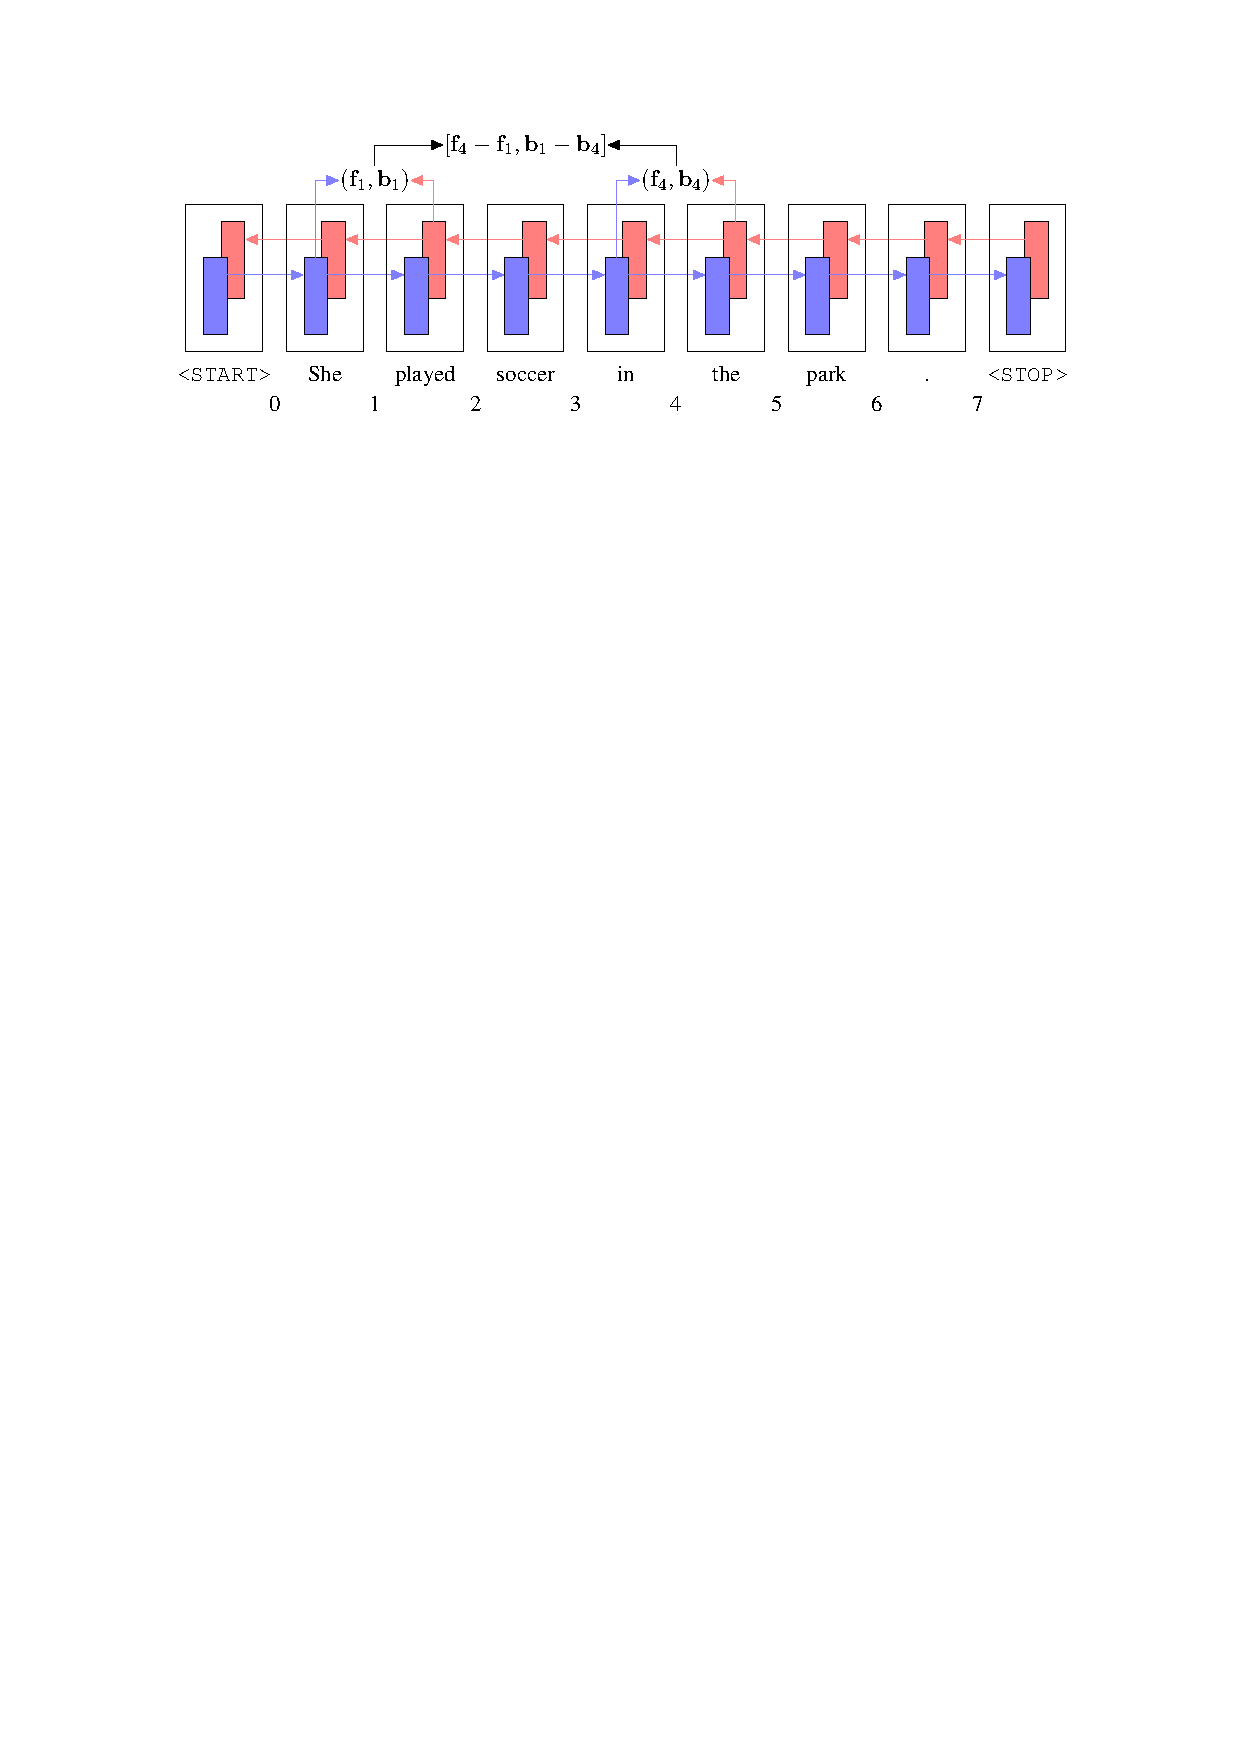
\includegraphics[width=\textwidth]{span-encoding.pdf}
    \caption{Representation for the span $(1, 4)$ computed from RNN encodings. Figure taken from \citet{stern2018analyis}.}
    \label{fig:span-feature}
  \end{figure}

\section{Inference}
  \label{sect:inference}
  Because our model is span-factored it allows efficient inference. In this section we describe efficient solutions to four related problems:
  \begin{itemize}
    \item Compute the normalizer $Z(\x) = \sum_{ \y \in \yieldx } \prod_{ a=1 }^{ A } \psi( \x, \y_a )$.
    \item Find the best parse $\hat{ \y } = \arg \max_{\y } p(\y  \mid \x)$
    \item Sample a tree $Y \sim P(Y \mid X = x)$.
    \item Compute the entropy $\entropy(Y \mid X = x)$ over parses for $\x$.
  \end{itemize}
  These problems can be solved by instances of the \textit{inside algorithm} and \textit{outside algorithm} \citep{baker1979trainable} with differentent semirings, an insight we take from semiring parsing \citep{goodman1999semiring}. In the following derivations we will make use of the notion of a \textit{weighted hypergraph} as a compact representation of all parses and their scores \citep{gallo1993directed,klein2004parsing}, and use some of the ideas and notation of \textit{semiring parsing} \citep{goodman1999semiring,eisner2009semirings}. First we describe the structure of the parse forest specified by our CRF parser, and then derrive the particular form of the inside and outside recursions for this hypergraph from the general formulations. We refer the reader to appendix \ref{A3-crf} for background on these ideas, and the introduction of the notation.

  \subsection{Weighted parse forest}
    The the CRF parser defines a hypergraph $G = (\mathcal{V}, \mathcal{E})$ with the following structure. We treat the dummy label $\varnothing \in \Lambda$ as any other label, unless we explictly indicate otherwise.

    The set $\mathcal{V}$ is defined relative to the sentence $\x$, and contains the invidual words of a sentence $\x$, together with all possible labeled spans over that sentence:
    \begin{align*}
      \mathcal{V} = \Big\{ \x_i \; \Big\vert \; 1 \leq i \leq n \Big\} \cup \Big\{ (A, i, j) \; \Big\vert \; A \in \Lambda, 0 \leq i < j \leq n \Big\} \cup \Big\{ (S^{\dagger}, 0, n) \Big\},
    \end{align*}
    where $(S^{\dagger}, 0, n)$ is a designated root node. The dependence on $x$ can be made explicit by writing $\mathcal{V}(x)$.

    The set of hyperedges $\mathcal{E} \subseteq 2^{\mathcal{V}} \times \mathcal{V}$ specifies all the ways that adjacent constituents can be combined to form a larger constituent, under a particular grammar. The edges connect sets of nodes at the \textit{tail} with a singel node at the \textit{head}. Because we (implicitly) assume a normal form grammar that contains \textit{all} possible productions, the set of hyperedges is particularly regular: the set $\mathcal{E}$ contains all edges that connect nodes $(B, i, k)$ and $(C, k, j)$ at the tail with $(A, i, j)$ at the head for all $0 \leq i < k < j \leq n$, all edges that connect $\x_i$ to $(A, i, i+1)$, and all labels can appear in the top node, with the exception of the dummy label $\varnothing$:
    \begin{align*}
      \mathcal{E}
        &= \Bigg\{ \Big\langle \Big\{ (B, i, k), (C, k, j) \Big\},  (A, i, j) \Big\rangle \; \Bigg\vert \; A, B, C \in \Lambda, \; 0 \leq i < k < j \leq n \Bigg\}  \\
        &\quad\cup \Bigg\{ \Big\langle \{ \x_i \}, (A, i-1, i) \Big\rangle \; \Bigg\vert \; A \in \Lambda, \; 1 \leq i \leq n \Bigg\}  \\
        &\quad\cup \Bigg\{ \Big\langle \{ (A, 0, n) \}, (S^{\dagger}, 0, n) \Big\rangle \; \Bigg\vert \; A \in \Lambda \setminus \{ \varnothing \} \Bigg\}
    \end{align*}
    The three kind of edges that make up $\mathcal{E}$ are illustrated in figure \ref{fig:crf-edges}. A tree is a set of nodes $y \subseteq \mathcal{V}(x)$, and the parse forest a set of trees $\yieldx \subseteq 2^{\mathcal{V}(x)}$.

    \begin{figure}[h]
      \center
      \begin{tikzpicture}[scale=.6]
        % \documentclass[11pt]{article}
% \usepackage{tikz}
% \usepackage{amsmath,amssymb,amsfonts}
%
% \usetikzlibrary{arrows,calc}
%
% \begin{document}

% \tikzstyle{every node}=[circle, draw, inner sep=0pt, minimum size=7mm]
%
% \tikzstyle{every node}=[circle, draw, inner sep=0pt, minimum size=11mm, node distance =1 cm and 1cm ]

% \begin{tikzpicture}

\node(a){$x_i$} ;
\node(b) at ($(a)+(4.5,0)$){$B_{i}^{k}$} ;
\node(c) at ($(b)+(3,0)$){$C_{k}^{j}$} ;
\node(d) at ($(c)+(4.5,0)$){$A_{0}^{n}$} ;

\node(A1) at ($(a)+(0,3)$){$A_{i-1}^{i}$} ;
\node(A2) at ($(b)+(1.5,3)$){$A_{i}^{j}$} ;
\node(S) at ($(d)+(0,3)$){$S^{\dagger n}_{0}$} ;

\draw[->] (a) to [in=-90,out=90](A1);

\draw[->] (b) to [in=-90,out=90](A2);
\draw[->] (c) to [in=-90,out=90](A2);

\draw[->] (d) to [in=-90,out=90](S);

% \end{tikzpicture}
%
% \end{document}

      \end{tikzpicture}
      \caption{The edge-types making up the hypergraph. The edges are instatiated for all $A, B, C \in \Lambda$ and all $0 \leq i < j \leq n$. Only for the rightmost edge holds the restriction $A \neq \varnothing$, to ensure that the dummy label cannot be the top node.}
      \label{fig:crf-edges}
    \end{figure}

    We connect a semiring $\mathcal{K}$ to the hypergraph by defining the weight function as $\omega: \mathcal{E} \to \mathbb{K}$, and by accumulating the weights with its binary operations. The function $\omega$ that assigns weights to the edges is given by either the function $\psi$ or $(\log \circ \, \psi)$, depending on the semiring used. Because of this association, the function $\omega$ has a very particular property: the function effectively depends only on the \textit{head} of the edge. Given edges $e = \langle \{ u, w \}, v \rangle$ and $e' =  \langle \{ u', w' \}, v \rangle$ for $u \neq u'$ and $w \neq w'$, their weights are equal: $\omega(e) = \omega(e')$. For this reason we write $\omega(v)$ instead.\footnote{Thus implicitly defining $\omega: \mathcal{V} \to \mathbb{K}$.} This fact will allow us to greatly simplify the recursions that follow. Additionally, this means that instead of computing independent scores for each of the $O(n^3 \vert\Lambda\rvert^3)$ edges, we only need to compute scores for the $O(n^2 \vert\Lambda\rvert)$ vertices. For a scoring function like a neural network, for which computation can be relatively expensive, this will make a significant difference.

   With this structure in place, we are ready to derive the form of the inference algorithm particular to this structure.

  \subsection{Inside recursion}
    The inside recursion computes quantities $\alpha(A,i,j)$ for all labels $A \in \Lambda$ and all spans $0 \leq i < j \leq n$ with respect to a semiring. What the quantity represents depends on the semiring used. In this section we derive the inside recursion specific to our hypergraph from the general result given.

    Let $\mathcal{K}$ be some semiring with binary operations $\oplus$ and $\otimes$ and identity elements $\bar{0}$ and $\bar{1}$. The inside recursion is given by the formula \citep{goodman1999semiring}
    \begin{align*}
      \alpha(v) =
        \begin{cases}
          \bar{1}  &  \mbox{if } I(v) = \varnothing,  \\
          \displaystyle\bigoplus_{e \in I(v)} \omega(e) \otimes \displaystyle\bigotimes_{u \in T(e)} \alpha(u)  & \mbox{otherwise.}
        \end{cases}
    \end{align*}
    Here $I(v) \subseteq E$ is the set of edges incoming at node $v$, and $T(e) \subseteq V$ is the set of nodes in the tail of edge $e$.

    At a node $v = (A, i, i+1)$ that spans one word $x_i$, the inside value is just the weight of the single edge incoming from that word:
    \begin{align}
        \label{eq:inside-base}
        \alpha(A, i, i+1) = \omega(A, i, i+1) \otimes \alpha(x_i) = \omega(A, i, i+1),
    \end{align}
    for $A \in \Lambda$, for all $0 \leq i < n$. We used the fact that $\alpha(x_i) = \bar{1}$, which follows from the fact that there are no arrows incoming at $\x_i$.

    For a general node $\alpha(A, i, j)$, $j > i + 1$, we observe that all the incoming edges have at the tail the nodes $(B, i, k)$ and $(C, k, j)$, for all $B, C \in \Lambda$ and $i < k < j$. The sum over edges thus reduces to independent sums over $B$, $C$, and $k$, and the product over the inside values at the tail reduces to the product of values $\alpha(B, i, k)$ and $\alpha(C, k, j)$. The form of $\omega$ allows us to rewrite this greatly as
    \begin{align}
      \label{eq:inside}
      \alpha(A, i, j)
        &= \bigoplus_{B \in \Lambda} \bigoplus_{C \in \Lambda} \bigoplus_{k=i+1}^{j-1} \omega(A, i, j) \otimes \alpha(B,i,k) \otimes \alpha(C,k,j) \nonumber \\
        &= \omega(A, i, j) \otimes \bigoplus_{k=i+1}^{j-1} \bigoplus_{B \in \Lambda} \alpha(B,i,k) \otimes \bigoplus_{C \in \Lambda} \alpha(C,k,j) \nonumber \\
        &= \omega(A, i, j) \otimes \bigoplus_{k=i+1}^{j-1} \sigma(i,k) \otimes \sigma(k,j),
    \end{align}
    where we have introduced the notational abbreviation
    \begin{align*}
        \sigma(i,j) &= \bigoplus_{A \in \Lambda} \alpha(A,i,j).
    \end{align*}
    Looking at \ref{eq:inside} we can see the marginalized values $\sigma(i, j)$ are all that are needed for the recursion. This suggest simplifying the recursion even further as
    \begin{align}
      \label{eq:inside-simplified}
      \sigma(i, j)
        &= \bigoplus_{A \in \Lambda} \alpha(A,i,j) \nonumber \\
        &= \Bigg[ \bigoplus_{A \in \Lambda} \omega(A, i, j) \Bigg] \otimes \Bigg[\bigoplus_{k=i+1}^{j-1} \sigma(i,k) \otimes  \sigma(k,j) \Bigg],
    \end{align}
    where we put explicit brackets to emphasize that independence of the subproblems of labeling and splitting.

    These values can be computed by visiting the nodes of the parse forest in topological order. This order ensures that the quantities in the tail of an edge will have been computed when the value at the node at the head is at turn. Given the highly regular form of the parse forest, this order boils down to something quite simple: the nodes are visited by increasing width of the span; the order in which the starting-points are visited does not matter because these nodes are not connected among each other.\footnote{\textit{Cf.} figure \ref{fig:hypergraph} in appendix \ref{A3-crf}: the width of the span determines the vertical level of the node in the parse forest; for a fixed width, the label and startpoint are all unconnected along this vertical level, and thus independent.}. We choose to visit the starting points from left to right, that is, from 0 to $n$.

  \subsection{Outside recursion}
    The outside algorithm computes the quantities $\beta(A,i,j)$ for all labels $A \in \Lambda$ and all spans $0 \leq i < j \leq n$. The general recursion is given by:
    \begin{align*}
      \beta(v) =
        \begin{cases}
          \bar{1}  & \mbox{if } O(v) = \varnothing, \\
          \displaystyle\bigoplus_{e \in O(v)} \omega(e) \otimes \beta(H(e)) \otimes \displaystyle\bigotimes_{ \substack{ w \in T(e) \\ w \neq u } } \alpha(w)  & \mbox{otherwise.}
        \end{cases}
    \end{align*}
    Here, $O(v) \subseteq E$ is the set of edges outgoing from $v$, $\ie$ the edges for which $v$ is in the tail, and define $H(e) \in V$ as the node at the head of edge $e$.

    The only node without outgoing edges is the root node, and thus
    \begin{align*}
      \beta(S^{\dagger}, 0, n) = \bar{1}.
    \end{align*}
    To compute $\beta(A, i, j)$ in the general case we need to sum over all outgoing edges. These come in two kinds: either $(A, i, j)$ combines with $(C, j, k)$ to form constituent $(B, i, k)$; or $(A, i, j)$ combines with $(C, k, i)$ to form constituent $(B, k, j)$. This corresponds to the following expression, that we can simplify by making use of the properties of $\omega$:
    \begin{align*}
      \beta(A, i, j)
        &= \bigoplus_{B \in \Lambda} \bigoplus_{C \in \Lambda} \bigoplus_{k=1}^{i-1} \omega(B, k, j) \otimes \alpha(C, k, i) \otimes \beta(B, k, j) \\
          &\qquad \oplus \bigoplus_{B \in \Lambda} \bigoplus_{C \in \Lambda} \bigoplus_{k=j+1}^{n} \omega(B, i, k) \otimes \beta(B, i, k) \otimes \alpha(C, j, k) \\
        &=  \bigoplus_{k=1}^{i-1}  \Bigg[ \bigoplus_{B \in \Lambda} \omega(B, k, j)  \otimes \beta(B, k, j) \Bigg] \otimes \Bigg[ \bigoplus_{C \in \Lambda} \alpha(C, k, i) \Bigg] \\
          &\qquad \oplus \bigoplus_{k=j+1}^{n}  \Bigg[ \bigoplus_{B \in \Lambda}  \omega(B, i, k) \otimes \beta(B, i, k) \Bigg] \otimes  \Bigg[  \bigoplus_{C \in \Lambda} \alpha(C, j, k) \Bigg] \\
        &=  \bigoplus_{k=1}^{i-1}  \sigma'(k, j) \otimes \sigma(k, i) \oplus \bigoplus_{k=j+1}^{n} \sigma'(i, k) \otimes  \sigma(j, k) \\
    \end{align*}
    where
    \begin{align*}
        \sigma(i, j) &= \bigoplus_{A \in \Lambda} \alpha(A, i, j),  \\
        \sigma'(i, j) &= \bigoplus_{A \in \Lambda} \omega(A, i, j) \beta(A, i, j).
    \end{align*}

    These values can be computed by visiting the nodes of the parse forest in \textit{reverse} topological order, exactly the opposite of the inside recursion. This order ensures that the quantities in the head of an edge will have been computed when the values in the tail are at turn. Again, this this order boils down to something quite simple: the nodes are visited based by decreasing width of their span, and again the order of the start-points are free.

  \subsection{Solutions}
    Equiped with the two recursions and a handful of semirings we can provide the solutions promised at the outset of this section.

    \paragraph{Normalizer}
      When we intantiate the inside recursion with the real semiring, the value of $\alpha$ at the root is the normalizer:
      \begin{align*}
        \alpha(\text{S}^{\dagger}, 0, n) = Z(\x),
      \end{align*}
      and when we instantiate the inside recursion with the log-real semiring we obtain the log-normalizer
      \begin{align*}
        \alpha(\text{S}^{\dagger}, 0, n) = \log Z(\x).
      \end{align*}

    \paragraph{Parse}
      To find the viterbi tree $\hat{ \y } = \arg \max_{ \y } p(\y  \mid \x)$ and its probability $p(\hat{\y} \mid \x)$ we use the Viterbi semirings ($\cf$ examples \ref{ex:vit-weight} and \ref{ex:vit-derivation} in appendix \ref{A3-crf}). We take equation \ref{eq:inside-simplified} and use the Viterbi semiring operations to derive that the value of the best subtree spanning words $i$ to $j$ is given by
      \begin{align}
        \label{eq:viterbi-score}
        \sigma(i,j)
          &= \max_{A} [ \log \psi(A, i, j) ] + \max_{k} [\sigma(i,k) + \sigma(k,j)].
      \end{align}
      The value $\log \Psi(\x, \hat{\y})$ is then given by $\sigma(0, n)$, and  can be normalized with to give the probability
      \begin{align}
        \log p(\hat{y} \mid x) = \sigma(0, n) - \log Z(x).
      \end{align}
      The best label and splitpoint $\hat{A}$ and $\hat{k}$ for the span $(i, j)$ are obtained by using the argmax:
      \begin{align}
        \label{eq:viterbi-tree}
        \hat{A} &= \argmax_{ A  } \log \psi(A, i, j)  \\
        \hat{k} &= \argmax_{ k } \sigma(i, k) + \sigma(k, j),
      \end{align}
      and the best tree $\hat{y}$ is found by following back from the root down to the leaves the best splits and labels.

    \paragraph{Sample}
      Unbiased samples from the model can be obtained by recursively sampling incoming edges, starting at the root node $(S^{\dagger}, 0, n)$, ending at the word nodes. The probability of an edge is proportional to the weight of all the trees under that edge. This is precicely what is represented by the inside value $\alpha$ computed in the real-semiring. At node $v = (A, i, j)$ the probability of edge $e = \langle \{ u, w \}, v \rangle$, with $u = (B, i, k)$ and $w = (C, k, j)$, is thus
      \begin{align}
        \label{eq:sample}
        P(E = e \mid V = v)
          &= \frac{\omega(e) \otimes \bigotimes_{u \in T(e)} \alpha(u)}{\alpha(v)}  \nonumber  \\
          &= \frac{\psi(A, i, j) \, \alpha(B, i, k) \, \alpha(C, k, j)}{\alpha(A, i, j)}.
      \end{align}
      Once an edge is sampled, the process is repeated at the nodes in the tail of that edge. We stop when we reach the nodes that span individual words. The sampled edges together then are guaranteed to form a tree. From a compuational point of view, this sampling is very efficient: the scores for the labeled spans need to be computed only once, followed by a single run of the inside and outside algorithm. Beyond this point, no costly computation is required. In our case, where the scores are predicted by a neural network, this means that we need to perfom just a single forward pass. Compare this with a sequential model such as the discriminative RNNG, where each sample requires an separate forward pass.

    \paragraph{Entropy}
      % To compute the entropy $H(Y \mid X = x)$ we need to first introduce the notion of the \textit{maginal probablity} of a node. The marginal of a node $v = (A, i, j)$ in a hypergraph is the probability that it occurs in a tree $\y$ for the sentence $\x$ as governed by the distribution $p$ that we defined on it. Let $V$ be a random variable with the hypergraph nodes $\mathcal{V}(x)$ as sample space, and define
      % \begin{align}
      %   P(V = v \mid X = \x)
      %     &\defeq \expect_Y[ \indicator_{ \{ v \in Y \} } ]  \nonumber \\
      %     &= \sum_{ \y \in \yieldx } p(\y \mid \x) \indicator_{ \{ v \in y \} }.
      % \end{align}
      %
      % The marginals can be computed from the inside and outside values computed in the real semiring as
      % \begin{align}
      %   P(V = v \mid X = \x) = \frac{\alpha(A, i, j) \, \beta(A, i, j)}{Z(\x)},
      % \end{align}
      % a result from \citep{goodman1999semiring}.\footnote{This can also be seen by noting that the product of $\alpha(A, i, j)$ and $\beta(A, i, j)$ is the sum over all trees that contain the node $v$, and $Z(\x)$ the sum over all trees in general.} The entropy can then be written as an expectation with respect to these marginals:
      % \begin{align}
      %   H(Y \mid X = x)
      %     &= - \sum_{ \y \in \yieldx } p(\y \mid \x) \log p(\y \mid \x)  \nonumber \\
      %     &= \log Z(\x) - \sum_{ \y \in \yieldx } p(\y \mid \x) \sum_{v \in \y} \log \psi(\x, v)  \nonumber \\
      %     &= \log Z(\x) - \sum_{ \y \in \yieldx } p(\y \mid \x) \sum_{ v \in \mathcal{V}(x) } \indicator_{ \{ v \in y \} } \log \psi(\x, v)  \nonumber \\
      %     &= \log Z(\x) - \sum_{ v \in \mathcal{V}(x) } \log \psi(\x, v)  \sum_{ \y \in \yieldx } \indicator_{ \{ v \in y \} } p(\y \mid \x)  \nonumber \\
      %     &= \log Z(\x) - \sum_{ v \in \mathcal{V}(x) } \log \psi(\x, v)  P(V = v \mid X = \x)  \nonumber \\
      %     &=  \log Z(\x) - \expect_V [ \log \psi(\x, V) ].
      % \end{align}
      To compute the entropy $\entropy(Y \mid X = x)$ we need to first introduce the notion of a \textit{node maginal}. The marginal of a node $v = (A, i, j)$ in a hypergraph is the probability that it occurs in a tree $\y$ for the sentence $\x$, according to the probability distribution $p$ over trees. The node marginal $\mu(v)$ is defined as the expectation
      \begin{align}
        \label{eq:node-marginal}
        \mu(v)
          &\defeq \expect[ \indicator( v \in Y ) ]  \nonumber \\
          &= \sum_{ \y \in \yieldx } p(\y \mid \x) \indicator( v \in y ).
      \end{align}
      This can be computed from the inside and outside values computed in the real semiring as
      \begin{align}
        \mu(v) = \frac{\alpha(A, i, j) \, \beta(A, i, j)}{Z(\x)},
      \end{align}
      a result from \citep{goodman1999semiring}. This can also be seen by noting that the product of $\alpha(A, i, j)$ and $\beta(A, i, j)$ is the sum over all trees that contain the node $v$, and $Z(\x)$ the sum over all trees in general.

      The entropy, then can then be written in terms of these marginals:
      \begin{align}
        \label{eq:crf-entropy}
        \entropy(Y \mid X = x)
          &= - \sum_{ \y \in \yieldx } p(\y \mid \x) \log p(\y \mid \x)  \nonumber \\
          &= \log Z(\x) - \sum_{ \y \in \yieldx } p(\y \mid \x) \sum_{v \in \y} \log \psi(\x, v)  \nonumber \\
          &= \log Z(\x) - \sum_{ \y \in \yieldx } p(\y \mid \x) \sum_{ v \in \mathcal{V}(x) } \indicator( v \in y ) \log \psi(\x, v)  \nonumber \\
          &= \log Z(\x) - \sum_{ v \in \mathcal{V}(x) } \log \psi(\x, v)  \sum_{ \y \in \yieldx } \indicator( v \in y ) p(\y \mid \x)  \nonumber \\
          &= \log Z(\x) - \sum_{ v \in \mathcal{V}(x) } \log \psi(\x, v) \mu(v)
      \end{align}

\section{Training}
  The CRF is trained to maximize the log likelihood of a labeled dataset $\dataset$ of pairs $(\x, \y)$
  \begin{align*}
    \mathcal{L}(\theta)
      &= \sum_{(\x, \y) \in \dataset} \log \ptheta(\y \mid \x)
  \end{align*}
  with respect to the model parameters $\theta$.

    Writing out the objective for a single example as
    \begin{align*}
      \log \ptheta(\y \mid \x) = \log \Psi(\x, \y) - \log Z(x)
    \end{align*}
    reveals that the maximization of this value decomposes as two separate optimizationproblems: to maximize the log-score of the example tree $\log \Psi(\x, \y)$, whilst minimizing the log of the total weight of the parse forest $\log Z(x)$. The solution is thus to move probability mass onto the gold tree $\y$, and away from \textit{all other trees}. Because the log-score of the tree decomposes as a sum of log-scores of the nodes that it comprises, the objective is effectively to \textit{increase} the scores of the labeled spans that make up the gold tree, and \textit{decrease} the scores of all other labeled spans not observed. Another effect of this factorization into spans is that such an update increases not only the probability of the gold tree, but the probability of all trees that share substantial substructure. It is in this precise sense that we mean that the model learns about all substructures.

    We rely on automatic differentiation to compute the derivatives, but note that in principle it is possible to efficiently combine the computation of the inside and outside values with their derivatives, a fact demonstrated in \citep{eisner2009semirings} and \citep{eisner2016backprop}, and implemented in \citep{kim2017structured}.\footnote{Amongst others, we do not take because it would require us to implement custom gradient computations in our toolkit of choice Dynet \cite{neubig2017dynet}, which is far from trivial.}

    It is fruitful to see how our global objective differs from the margin-based objective in \citep{stern2017minimal}. The margin-based objective is to maximize the difference, or `margin', between the score of the gold tree and the highest scoring, incorrect tree. Given a sentence $\x$ the model computes the predicted tree $\hat{y}$. If the predicted tree equals the gold tree, $\hat{y} = \y$, then no changes to the model parameters are made. Otherwise, the model parameters are updated to maximize the difference between their scores
    \begin{align*}
      \log \Psi(\x, \y) - \log \Psi(\x, \hat{\y}),
    \end{align*}
    maximizing the score of the correct tree, and minimizing the score of the predicted tree.\footnote{The full objective reported in the paper is minimizing the hinge loss $\max \Big(0, 1 - \log \Psi(\x, \y) + \log \Psi(\x, \hat{\y}) \Big)$, and the above is what the actual implementation comes down to. Note that Viterbi ensures that for all $\y$, $\log \Psi(\x, \hat{\y}) \geq \log \Psi(\x, \y)$.} This objective shows a striking similarity with our CRF objective, with one very particular difference. The goal is still to maximize the score of the gold tree. But the minimization that in the CRF objective concerns all possible trees through $Z(x)$, in this objective concerns just the single tree $\hat{\y}$ that was incorrectly predicted. The scores of all other nodes not observed in either tree are not affected directly.

  % \subsection{Speed and complexity}
  %   The model is slow. Here we will describe how slow it is, and what can be done about it.
  %   \begin{itemize}
  %     \item During training the computation time is dominated by two computations: the forward pass with the neural networks that obtains the node scores, and the time complexity of the inside algorithm. The complexity of the and how it depends on both label size and sentence length
  %     \item Describe how slow the model is to train of CPU (use Lisa times): around 7 hours per epoch, so around 15 days for convergence (around 50 epochs).
  %     \item Describe how we can speed up linearly by pruning the labelset: we can remove 70\% of labels while keeping 98\% of the training sentences. These labels are mostly very rare unary chains. The speedup we get from this is linear!
  %     \item Our model is X times slower than the model of \citet{stern2017minimal}. This difference bust be in the inside algorithm. The inside algorithm used by us and the viterbi algorithm used by \citet{stern2017minimal} have the same structure and time complexity. The difference must be in the computation graph built by either computation. The viterbi algorithm builds a sparse computation graph, connecting only nodes that are in a single tree, whereas the computation graph built by the inside algorithm is dense with all trees.
  %   \end{itemize}

\section{Experiments}
  This section reports the results of the experiments performed with the CRF parser. We first train the model on the Penn Treebank and show that it is a strong parser. The CRF obtains a higher F1 than the discriminative RNNG when trained with the same number of parameters; an even higher F1 is obtained when or models is trained with the same hyperparameters as the model in \citet{stern2017minimal}. We then use the CRF as an alternative proposal model for the generative RNNG and perform analyses similar to those in chapter \ref{03-rnng}. This use of the CRF leads to some theoretical challenges. We note these, but discuss them in detail in the next section.

  \subsection{Setup}
    We train two versions of the model on the Penn Treebank: a small version and a large version. The smaller model allows us to compare the CRF parser to the discriminative RNNG, while the larger model allows us to compare it to the parser of \citet{stern2017minimal}. The smaller model has dimensions to match the number of parameters in the discriminative RNNG from chapter \ref{03-rnng} and is trained in the same way. For the larger model we follow the dimensions and optimization details of \citet{stern2017minimal}.

    For both models the embeddings are of dimension 100, and the LSTMs have 2 layers. For the smaller model the dimension of forward and backward the LSTM is 128, and the feedforward network has one hidden layer with dimension 256. For the larger model we follow the hyperparameters of \citet{stern2017minimal}: the LSTMs have dimesion 250, just as the feedforward network. Given these dimensions, the total number of parameters in the small model is around 0.75M and around 2.5M for the large model (the exact numbers are in table \ref{tab:num-params}). The small CRF is comparable in size with the discriminative RNNG (around 0.8M parameters) and less than a third in size of the larger model. The smaller model is optimized exactly as the discriminative RNNG: SGD with learning rate 0.1, and dropout of 0.2. For the larger model we use Adam \citep{kingma2014adam} with 0.001 and dropout of 0.4, exactly following \citet{stern2017minimal}.

  \subsection{Results}
    The evaluation setup is the same as in the previous chapter. We train 10 models from different random seeds, and we report mean and standard deviations, as well as scores of the best model selected by development F1.

    % \begin{table}[h]
% \center
% \footnotesize
%   \begin{tabular}{l|c|c|c|c}
%       & Small & Large & \citet{stern2017minimal} & \citet{stern2018analyis} word-only  \\ \hline
%     F1  & $89.94 \pm	0.12$ \quad (90.04) & $90.31 \pm 0.15$ \quad (90.43) &  -- \quad (91.79) &  -- \quad (91.44)
%   \end{tabular}
%   \caption{F1 scores for the CRF.}
%   \label{tab:disc-fscores}
% \end{table}

\begin{table}[h]
  \center
  \footnotesize
  \begin{tabular}{l|c|c|c}
      & Small & Large & \citet{stern2017minimal} \\ \hline
    F1  & $89.94 \pm	0.12$ \quad (90.04) & $90.31 \pm 0.15$ \quad (90.43) &  -- \quad (91.79)
  \end{tabular}
  \caption{F1 scores for the CRF.}
  \label{tab:disc-fscores}
\end{table}


    The results are shown in \ref{tab:crf-fscores}. Both models perform well, achieving on average 89.94 F1 for the smaller model and 90.31 F1 for the larger model. The small difference in F1 between the two is surprising given difference in size and optimization, and speaks for the relative robustness of our model with respect to these choices. Our best small CRF (90.04 F1) surpasses the best discriminative RNNG (88.58) by almost 2.5 F1, but our best large CRF (90.43) performs below the model of \citet{stern2017minimal} (91.79). Just as for the RNNG, we believe this can be attributed to the absence of tags. However, we can note that---in case this is true---the negative impact is much greater for the RNNG (around 3.1 F1 lower) than in the CRF (around 1.4 F1 lower).

  \subsection{Proposal distribution}
    We have introduced the CRF parser as an alternative proposal model for the generative RNNG, and we now evaluate the CRF in this role. We repeat the same inference procedure as in chapter \ref{03-rnng}: we sample 100 trees from the small CRF with the highest development F1, and use these to evaluate the same generative RNNG as before. The results are shown in tables \ref{tab:gen-fscores-crf} (F1) and \ref{tab:gen-perplexities-crf} (perplexity), and include the previous results for comparison.

    \begin{table}[h]
\center
\footnotesize
  \begin{tabular}{l|c|c|c}
      Proposals & Our RNNG & CRF & \citet{dyer2016rnng} &  \\ \hline
      Ours  & $91.07 \pm	0.1 \quad (91.12)$  &  $91.02 \pm 0.05 \quad (91.04)$ &  $93.32 \pm 0.1 \quad (93.32)$  \\
      \citet{dyer2016rnng}  & -- & -- & -- \quad (93.3)
  \end{tabular}
  \caption{F1 scores for the generative RNNG, for different proposal models. The first column is with proposals from our discriminative RNNG, the final column is with the proposals used by \citet{dyer2016rnng} to evaluate, availlable at \url{https://github.com/clab/rnng}.}
  \label{tab:gen-fscores}
\end{table}


    \begin{table}[h]
\center
\footnotesize
  \begin{tabular}{l|c|c|c}
       & RNNG & CRF & \citet{dyer2016rnng}  \\ \hline
      Our RNNG & $108.76 \pm	1.52 \quad (107.43)$  &  $117.79 \pm 2.1 \quad (116.28)$ &  $107.80 \pm 1.59 \quad (106.45)$  \\
      \citet{dyer2016rnng}  & -- & -- & -- \quad (105.2)  \\
      \citet{kuncoro2017syntax}  & -- & -- & -- \quad (100.9)
  \end{tabular}
  \caption{Perplexity on the PTB of the generative RNNG, for different proposal models.}
  \label{tab:gen-perplexities-crf}
\end{table}


    The results for the F1 are virtually the same. Although the CRF is the better parser by F1, both are equivalent with respect to generative RNNG. On average, however, because the discriminative RNNG proposals performs better on the selected model. A real difference can be observed in the perplexity, with a difference of over 9 nats in favour of the RNNG.

  \subsection{Analysis}

    We perform the same analyses of the approximate inference as in chapter \ref{03-rnng}, this time with the CRF as proposal model. The results of the experiment on aproximate inference are shown in figure \ref{fig:samples-fscores-crf} (F1) and \ref{fig:samples-perplexities-crf} (perplexity), where they are compared to the results of the annealed RNNG. With respect to parsing F1, the CRF is the better choice when using few samples, but for this difference disappears for larger number of samples.

    Figure \ref{fig:samples-entropy-crf} shows the estimation of the conditional entropy, now including the results for the CRF. The estimates of the CRF converge to the true conditional entropy, which can be computed exactly and equals 2.84.\footnote{To be precise, the values $\entropy(Y \mid X = x)$ can be computed exactly, the value $\entropy(Y \mid X)$ is still estimated by a mean over the test set.} Furthermore we can note that the conditional entropy of the CRF is higher than that of the discriminative RNNG when not annealed. This could indicate that the CRF maintains a higher number of alternative parses per sentence on average than the RNNG. Another plausible explanation is that the higher entropy is caused by the derivational ambiguity: the higher entropy reflects that each tree has multiple derivations.

    % \begin{figure}[h]
    %   \center
    % 	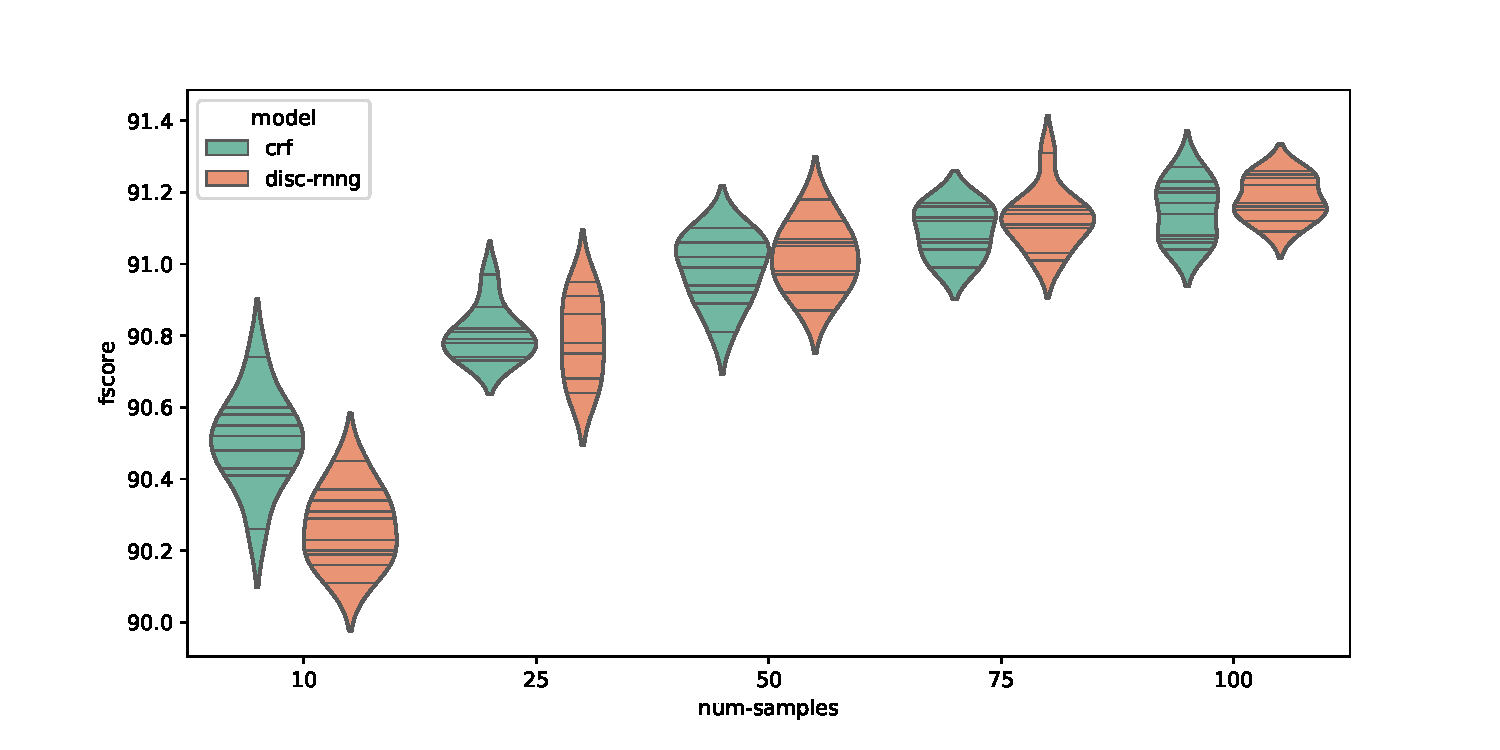
\includegraphics[width=0.9\textwidth]{sample-experiment/fscore/crf_disc_08.pdf}
    % \caption{F1 estimated with increasing number of samples, with CRF and discriminative RNNG annealed with $\alpha=0.8$, for 10 independent repetitions.}
    % \label{fig:samples-fscores-crf}
    % \end{figure}
    %
    % \begin{figure}[h]
    %   \center
    % 	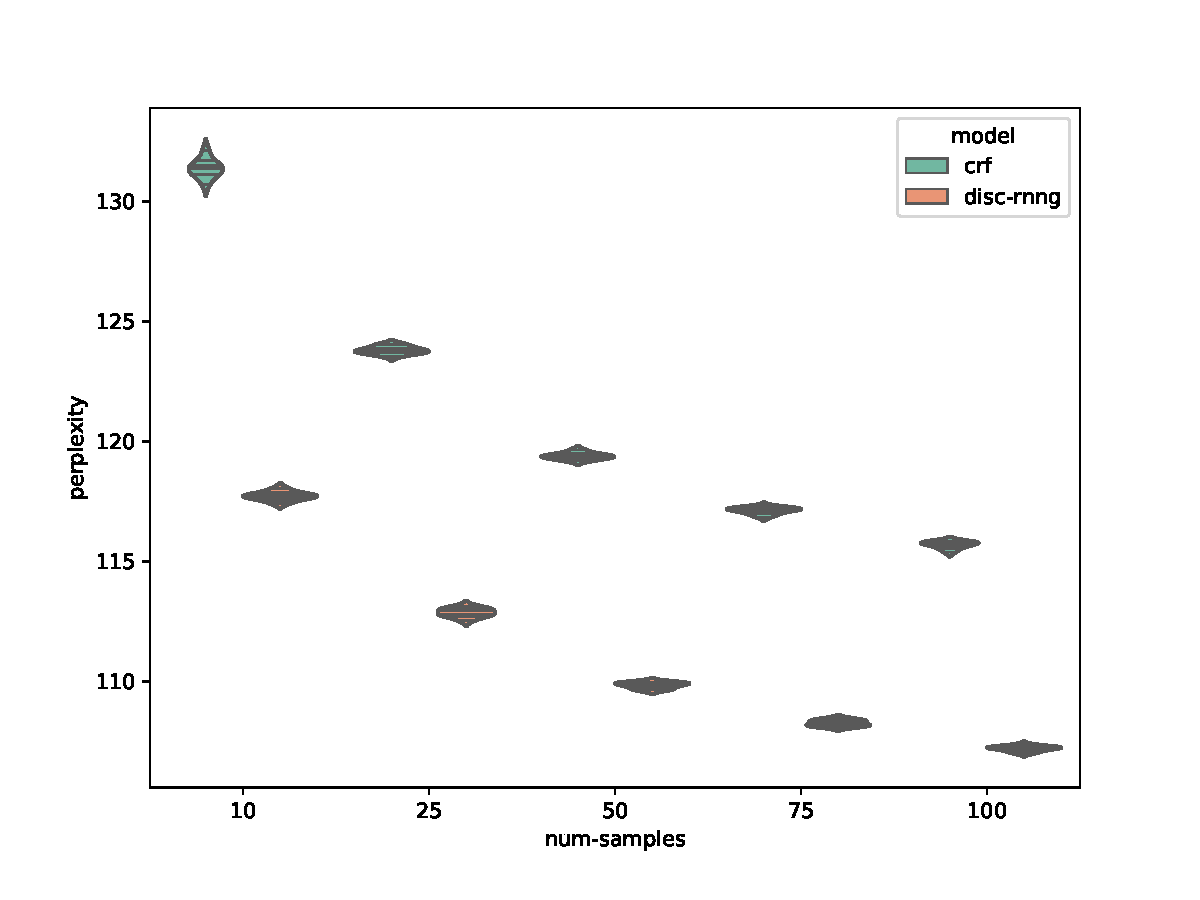
\includegraphics[width=0.7\textwidth]{sample-experiment/ppl/crf_disc08.pdf}
    % \caption{Perplexity estimated with increasing number of samples, with CRF and discriminative RNNG annealed with $\alpha=0.8$, for 10 independent repetitions.}
    % \label{fig:samples-perplexities-crf}
    % \end{figure}
    %
    % \begin{figure}[h]
    %   \center
    %   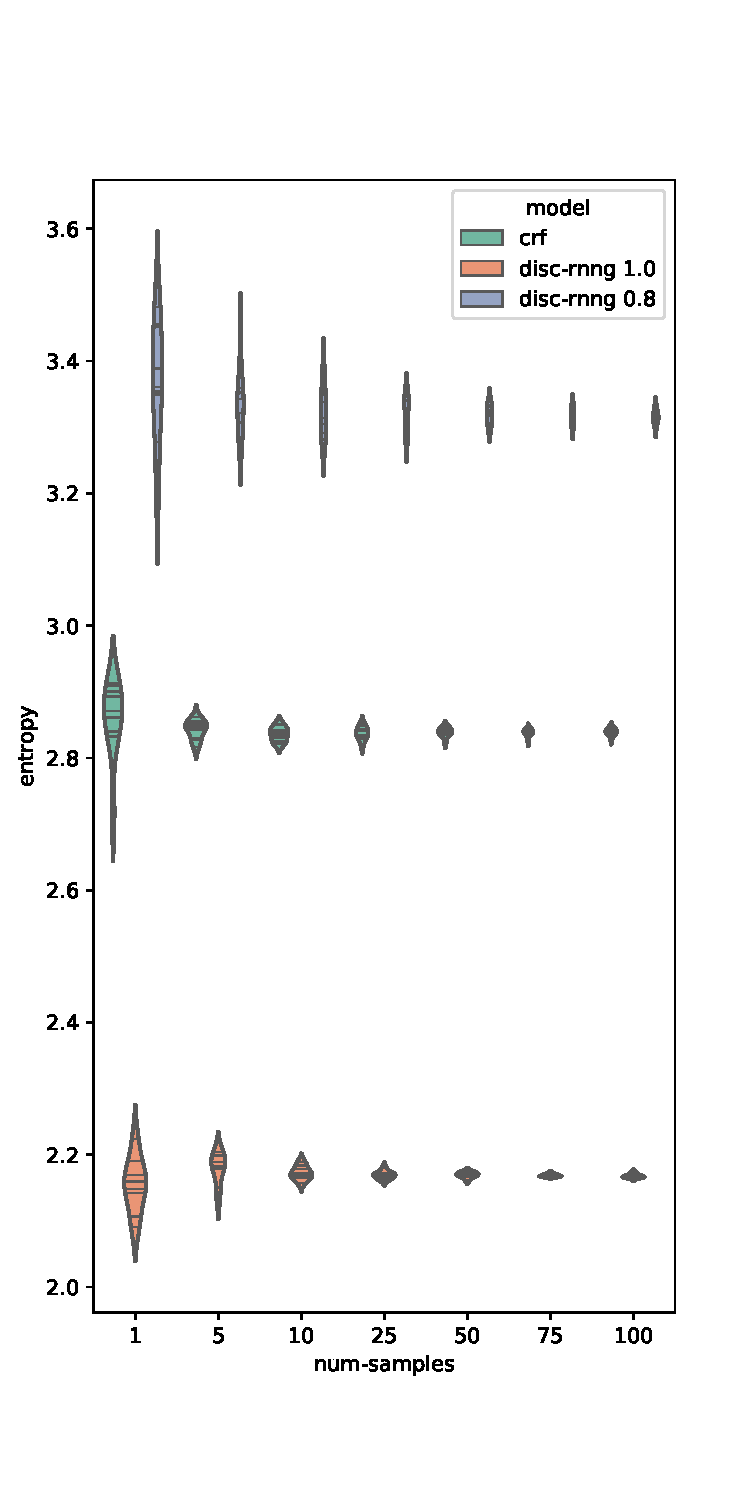
\includegraphics[width=0.4\textwidth]{sample-experiment/entropy/all.pdf}
    % \caption{Conditional entropy estimated with increasing number of samples.}
    % \label{fig:samples-entropy-crf}
    % \end{figure}

    \begin{figure}[h]
      \center
    	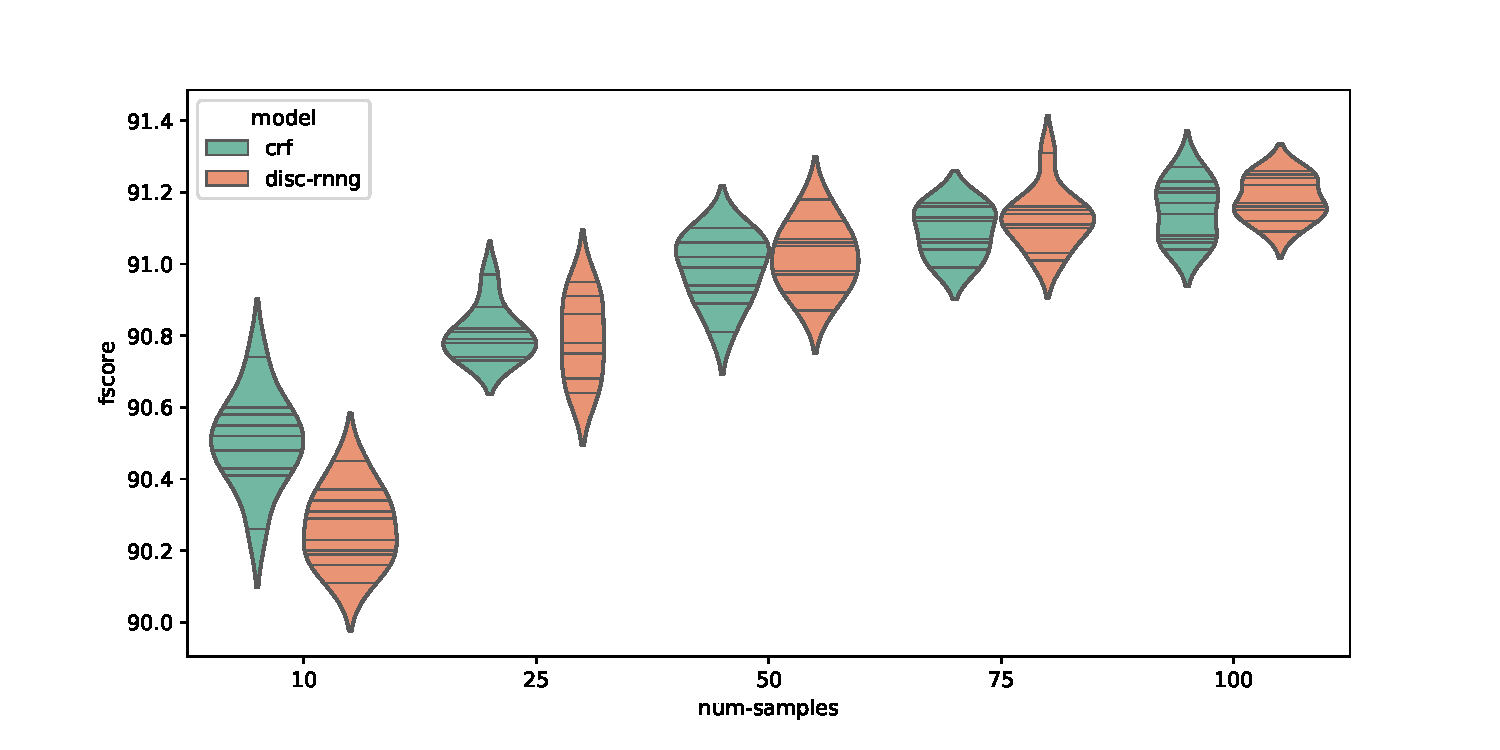
\includegraphics[width=0.9\textwidth]{sample-experiment/fscore/crf_disc_08.pdf}
      \caption{F1 estimated with increasing number of samples, with CRF and discriminative RNNG annealed with $\alpha=0.8$, for 10 independent repetitions.}
      \label{fig:samples-fscores-crf}
    \end{figure}

    \newgeometry{top=5mm, bottom=5mm}  % enables full page view
    \begin{figure}[h]
      \center
    	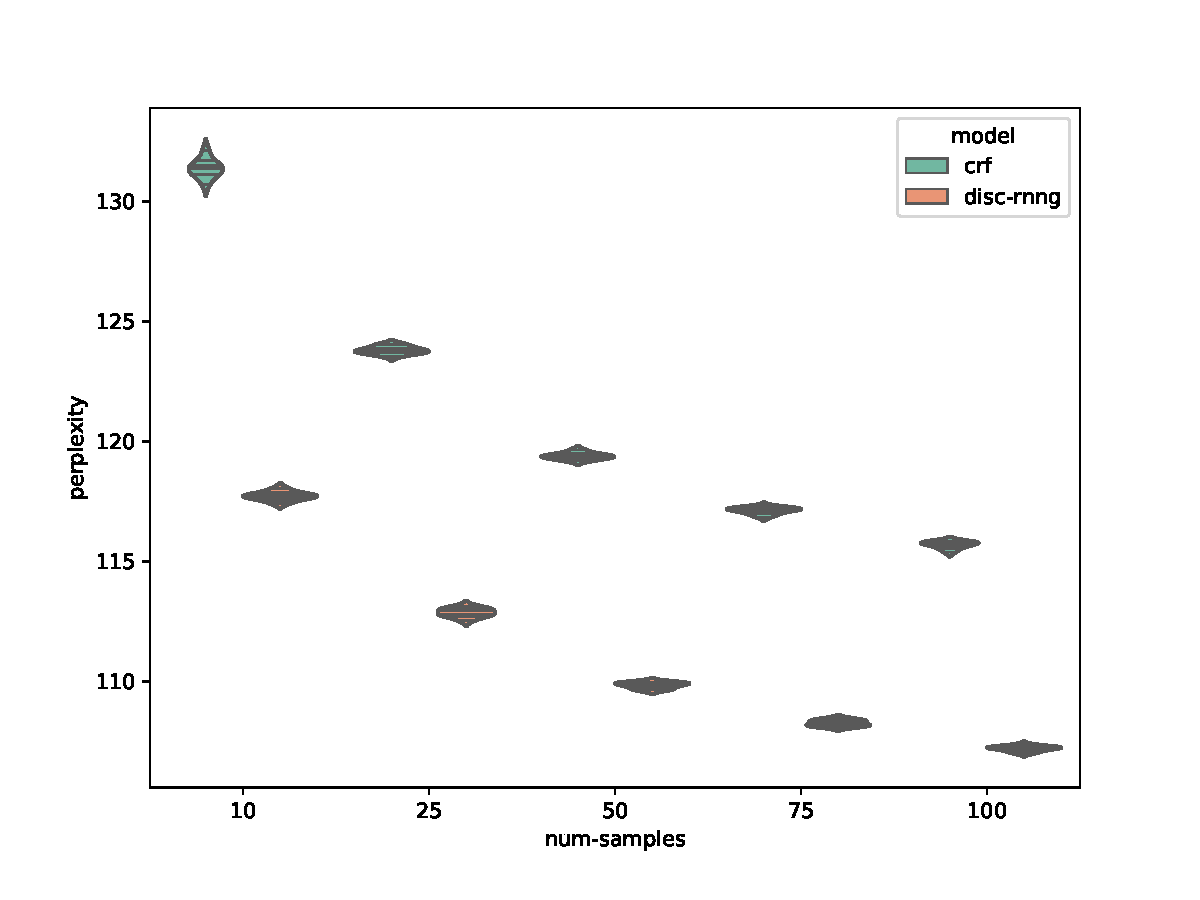
\includegraphics[width=0.8\textwidth]{sample-experiment/ppl/crf_disc08.pdf}
      \caption{Perplexity estimated with increasing number of samples, with CRF and discriminative RNNG annealed with $\alpha=0.8$, for 10 independent repetitions.}
      \label{fig:samples-perplexities-crf}

      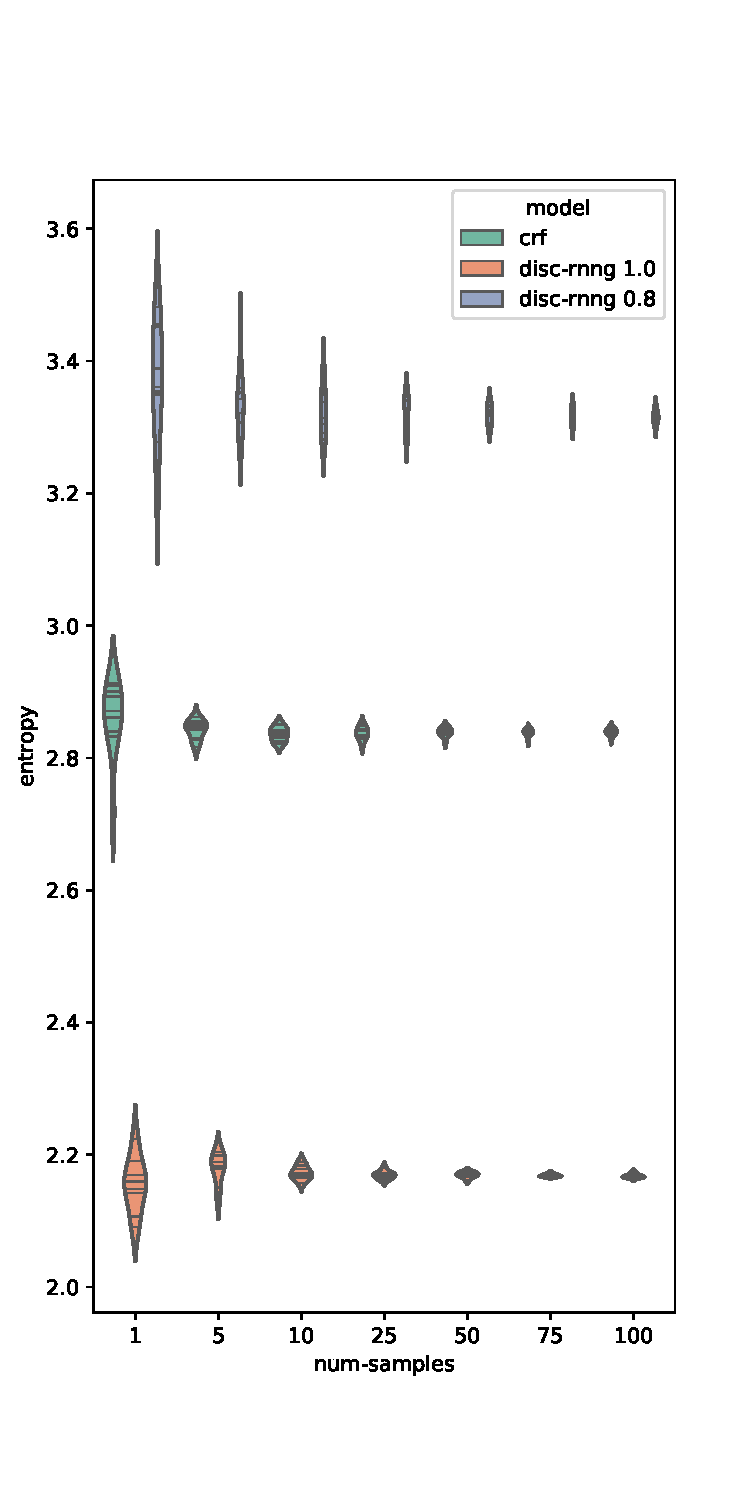
\includegraphics[width=0.5\textwidth]{sample-experiment/entropy/all.pdf}
      \caption{Conditional entropy estimated with increasing number of samples.}
      \label{fig:samples-entropy-crf}
    \end{figure}
    \restoregeometry

\section{Trees and derivations}
  The use of the CRF as a proposal distribution brings to light a subtle issue: by our choice of binarization we have introduced derivational ambiguity, and this affects the approximate marginalization. In this section we will describe the issue, which we characterize as the difference between the binary \textit{derivations} and the \textit{trees} they collapse to. We analyze the impact of this on the approximate marginalization, and then propose solutions. We will return to this difference in chapter \ref{05-semisupervised}, where the computation of the entropy plays a central role.

  \subsection{Derivational ambiguity}
    The way our CRF deals with binarization and its inverse introduces the problem derivational ambiguity: many binary derivation $d$ modelled by the CRF as distinct map to the same tree $y$ when the dummy node is collapsed. In other words: we map a treebank tree to a single normal form derivation, but many normal form derivations map to a that treebank tree. For example, the two normal form trees in \ref{fig:normal-form-trees} both collapse to the same tree when dummy labels $\varnothing$ are collapsed:
    \begin{center}
      (S (NP The other hungry cat) (VP meows) .).
    \end{center}
    However, when going the other way---applying the normal form transformation to the above tree---we always obtain the left tree, and never the right tree. Let $f: \yieldx \to \mathcal{D}(x)$ be the transformation that we defined that produces normal form trees from treebank trees, and let $g: \mathcal{D}(x) \to \yieldx$ be the transformation that takes a normal form tree and collapses the dummy nodes. Then $f$ is a bijection, but $g$ is not: for any tree $y$ the preimage of $g$ is the set of derivations $g^{-1}( y ) = D \subseteq \mathcal{D}(x)$ that collapse to the same tree. And generally, $\lvert D \rvert > 1$. This is the issue at hand: going from derivations to trees causes derivational ambiguity.

    \begin{figure}[h]
      \begin{subfigure}[b]{0.5\textwidth}
        \center
        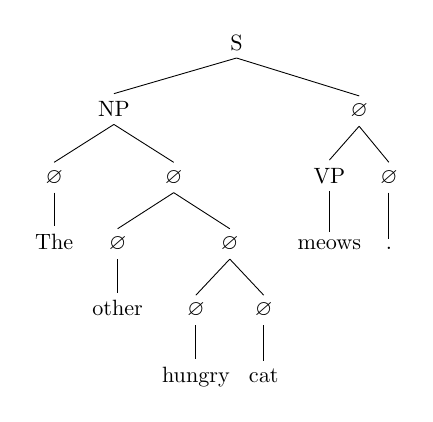
\begin{tikzpicture}[scale=.8]
          \Tree [.S
        [.NP
          [.$\varnothing$ The ]
          [.$\varnothing$ [.$\varnothing$ other ] [.$\varnothing$ [.$\varnothing$ hungry ] [.$\varnothing$ cat ] ] ] ]
        [.$\varnothing$ [.VP meows ] [.$\varnothing$ . ] ] ]

        \end{tikzpicture}
    	\end{subfigure}
    	\begin{subfigure}[b]{0.5\textwidth}
        \center
        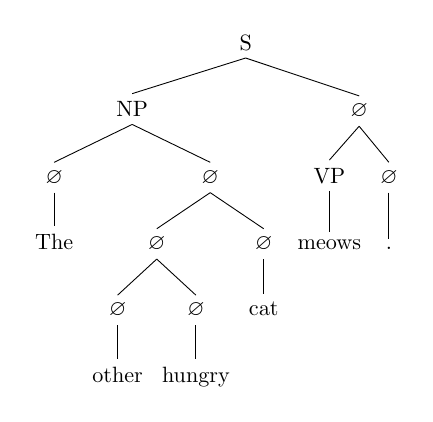
\begin{tikzpicture}[scale=.8]
          \Tree [.S
        [.NP
          [.$\varnothing$ The ]
          [.$\varnothing$ [.$\varnothing$ [.$\varnothing$ other ] [.$\varnothing$ hungry ] ] [.$\varnothing$ cat ] ] ]
        [.$\varnothing$ [.VP meows ] [.$\varnothing$ . ] ] ]

        \end{tikzpicture}
    	\end{subfigure}
      \caption{Two normal form derivations that collapse to the same tree.}
      \label{fig:normal-form-trees}
    \end{figure}

  \subsection{Consequences}
    The direct consequence of the derivational ambiguity is that our CRF actually defines a distribution over $\mathcal{D}(x)$, and over $\yieldx$ only through by summing over the derivations that collapse to it. Let $\y$ be a general tree such as is modelled by the RNNG. Our CRF assigns probabilities to all $d \in f^{-1}(y)$ and defines a distribution over $\yieldx$ through
    \begin{align*}
      p(y \mid x) = \sum_{d \in f^{-1}(y)} p(d \mid x).
    \end{align*}
    As a consequence $p(d \mid x) \leq p(y \mid x)$ for all of the derivations $d$ that collapse to $y$. This has three direct consequences:
    \begin{itemize}
      \item We overestimate the marginal probability in the importance sampling:
        \begin{align*}
          \frac{1}{K}\sum_{i=1}^K  \frac{\ptheta( \x, \y^{(i)} )}{\qlambda(d^{(i)} \mid \x)}
            &\geq \frac{1}{K}\sum_{i=1}^K  \frac{\ptheta( \x, \y^{(i)} )}{\sum_{d \in f^{-1}(y^{(i)})} \qlambda(d \mid \x)}  \\
            &= \frac{1}{K}\sum_{i=1}^K  \frac{\ptheta( \x, \y^{(i)} )}{\qlambda(\y^{(i)} \mid \x)}  \\
            &\approx \expect_{q} \bigg[\frac{\ptheta(\x,\y )}{\qlambda(\y \mid \x)} \bigg] = \ptheta(\x).
        \end{align*}
      \item Viterbi returns the best derivation, not necessarily the best tree. In other words, if $\hat{d} = \argmax_d p(d \mid \x)$ then $g(\hat{d}) \neq \argmax_y p(\y \mid \x)$ in general. This is a situation similar to decoding in latent variable PCFGs \citep{petrov2006learning}, which is known to be intractable \citep{sima2002computational}.
      \item The entropy is over derivations instead over trees, and it is not clear how one relates to the other.
    \end{itemize}
    The derivational ambiguity does not affect the samples: the probability that we draw $y$ is precisely the probability that we draw any $d$ in $f^{-1}(y)$.

  \subsection{Solutions}
    We propose two solutions to this problem:
    \begin{enumerate}
      \item We can dispense with the dummy label altogether, and instead alter our CRF so that it can deal directly with $m$-ary trees, for any order $m$. This means that we add all hyperedges with more than 2 children. The general formulation of the inside and outside recursions remain unaltered, but the specific form becomes less efficient because we now need to deal with a sum over all possible partitions of the span under a node.
      \item We keep the dummy label, but prune the hyperforest to only contain derivations that are reachable by the normal form transformation. This means that we assign probability zero to all trees that do not correspond to the cannonical normal form that we commited to by choosing the transformation. Because this transformation is very regular, we can easily incorporate this pruning in the inside and outside algorithms.
    \end{enumerate}

    We now describe either solution, starting with the solution of making the CRF deal directly with $m$-ary trees.

  \subsection{Unrestricted parse forest}
    One solution, as noted, is to make the parse-forest deal with $m$-ary trees directly. This requires that for each noterminal node, we add incoming edges that contain more than two children in the tail. This needs to be done for each permissible number of children---determined by the width of the span---and for all possible partitions of that size of the span.

    More formally, let $(A,i,j)$ be a node with $i + 1 < j$, so that it can expand to other noterminal nodes. Then let $i = k_0 < k_1 < k_2 < \cdots < k_m = j$ be a partition of the discrete interval $[i, j]$ into $m$ subspans. Since a span must have a width of at least 1, $m$ can be at most $j-i$ Letting $B_1, \dots, B_m$ be labels for those subspans we can form an edge that connects the set
    \begin{align*}
      \Big\{ (B_1, k_0, k_1), (B_2, k_1, k_2), \dots, (B_m, k_{n-1}, k_m) \Big\}
    \end{align*}
    at the tail to the node $(A, i, j)$ at the head. Adding \textit{all} such nodes to the parse forest for each $m$ will allow us to deal with trees of unrestricted arity directly.

    The generality of the semiring formulations of the inside and outside algorithms, allows us to seamlesly apply them to this new parse forest. If we let $v = (A, i, j)$ such that $I(v) \neq \varnothing$ we can derive the inside value $\alpha(v)$ as
    \begin{align*}
      \alpha(v)
        &= \displaystyle\bigoplus_{e \in I(v)} \omega(e) \otimes \displaystyle\bigotimes_{u \in T(e)} \alpha(u)  \\
        &= \displaystyle\bigoplus_{m = 2}^{j - i} \displaystyle\bigoplus_{k_0 < k_1 < \cdots < k_m} \displaystyle\bigoplus_{B_1 \in \Lambda} \cdots \displaystyle\bigoplus_{B_m \in \Lambda} \omega(A, i, j) \otimes \displaystyle\bigotimes_{l=1}^n \alpha(B_l, k_{l-1}, k_l) \\
        &= \omega(A, i, j) \otimes \displaystyle\bigoplus_{m = 2}^{j - i} \displaystyle\bigoplus_{k_0 < k_1 < \cdots < k_m} \displaystyle\bigotimes_{l=1}^n \displaystyle\bigoplus_{B \in \Lambda} \alpha(B, k_{l-1}, k_l) \\
        &= \omega(A, i, j) \otimes \displaystyle\bigoplus_{m = 2}^{j - i} \displaystyle\bigoplus_{k_0 < k_1 < \cdots < k_m} \displaystyle\bigotimes_{l=1}^n \sigma(k_{l-1}, k_l), \\
    \end{align*}
    where logic that allows us write
    \begin{align*}
      \displaystyle\bigoplus_{B_1 \in \Lambda} \cdots \displaystyle\bigoplus_{B_m \in \Lambda} \displaystyle\bigotimes_{l=1}^n \alpha(B_l, k_{l-1}, k_l) = \displaystyle\bigotimes_{l=1}^n \displaystyle\bigoplus_{B \in \Lambda} \alpha(B, k_{l-1}, k_l)
    \end{align*}
    is the same as in the binary case, but generalized to $m$ terms.

    For the outside value $\beta(v)$ we can follow a similar derivation. Let
    \begin{align*}
      0 \leq k_0 < \cdots < k_a = i < j = k_{a+1} < \cdots < k_m \leq n
    \end{align*}
    be a partition of the discrete interval $[k_0, k_m]$ into $m$ pieces, one of which is $[i, j]$, namely the interval $[k_a, k_{a+1}]$. This partition represents one way in wich the interval $[i, j]$ can be completed with $m-1$ other intervals into an interval $[k_0, k_m]$. With this in place, we can derive the outside recursion as
    \begin{align*}
      \beta(v)
        &= \displaystyle\bigoplus_{e \in O(v)} \omega(w) \otimes \beta(H(e)) \otimes \displaystyle\bigotimes_{ \substack{ w \in T(e) \\ w \neq u } } \alpha(w) \\
        &= \displaystyle\bigoplus_{m = 2}^{n - j + i} \displaystyle\bigoplus_{k_0=0}^{i-1} \displaystyle\bigoplus_{k_m = j}^{n} \displaystyle\bigoplus_{k_0 < \cdots < k_a < k_{a+1} < \cdots < k_m} \displaystyle\bigoplus_{B \in \Lambda}  \\
          &\qquad\qquad \omega(A, i, j) \otimes \beta(B, k_0, k_m) \otimes \displaystyle\bigotimes_{ \substack{1 \leq l \leq n \\ l \neq a } } \displaystyle\bigotimes_{C \in \Lambda} \alpha(C, k_{l-1}, k_l) \\
        &= \displaystyle\bigoplus_{m = 2}^{n - j + i} \displaystyle\bigoplus_{k_0=0}^{i-1} \displaystyle\bigoplus_{k_m = j}^{n} \displaystyle\bigoplus_{k_0 < \cdots < k_a < k_{a+1} < \cdots < k_m}  \\
          &\qquad\qquad \displaystyle\bigoplus_{B \in \Lambda} \omega(B, i, j) \otimes \beta(B, k_0, k_m) \otimes \displaystyle\bigotimes_{ \substack{1 \leq l \leq n \\ l \neq a } } \displaystyle\bigotimes_{C \in \Lambda} \alpha(C, k_{l-1}, k_l)  \\
        &= \displaystyle\bigoplus_{m = 2}^{n - j + i} \displaystyle\bigoplus_{k_0=0}^{i-1} \displaystyle\bigoplus_{k_m = j}^{n} \displaystyle\bigoplus_{k_0 < \cdots < k_a < k_{a+1} < \cdots < k_m} \sigma'(k_0, k_m) \otimes \displaystyle\bigotimes_{ \substack{1 \leq l \leq n \\ l \neq a } } \sigma(k_{l-1}, k_l).
    \end{align*}

    The above two recursions show that this approach is challenging, despite its elegance. Enumerating the sets of partitions is in itself already a nontrivial task.

  \subsection{Pruned parse forest}
    Another solution is to prune the parse forest: to keep only those trees that can be obtained by the normal form transformation. Going back to the example at the beginning of the example, this solution asks us to assign probability zero to the right tree, the tree that we cannot obtain by the normal form transformation. Since the transformation that we apply is very regular, we can easily characterize the set of trees that are impossible to derive. In fact, it boils down to one characteristic: a node can have the label $\varnothing$ only when \textit{either} that node spans a single word \textit{or} that node is the right child of its parent node.\footnote{We binarize \textit{rightwards}, thus introducting the dummy labels in that position, and can only ever introduce the dummy label in the left child position when it spans a single word.} That means we should remove from the parse forest all edges of the form illustrated in figure \ref{fig:illegal-edges}. By this same reasoning we conclude that the parse forest should also be rid of all nodes of the form $(\varnothing, 0, j)$ for $j > 1$, which cannot occur in any tree obtained with our transformation.

    \begin{figure}[h]
      \center
      \begin{tikzpicture}[scale=.6]
        % \documentclass[11pt]{article}
% \usepackage{tikz}
% \usepackage{amsmath,amssymb,amsfonts}
%
% \usetikzlibrary{arrows,calc}
%
% \begin{document}

% \tikzstyle{every node}=[circle, draw, inner sep=0pt, minimum size=7mm]
%
% \tikzstyle{every node}=[circle, draw, inner sep=0pt, minimum size=11mm, node distance =1 cm and 1cm ]

% \begin{tikzpicture}

\node(b){$\varnothing_{i}^k$} ;
% \node(b){$\varnothing_{i,k}$} ;
\node(c) at ($(b)+(2,0)$){$B_{k}^j$} ;
% \node(c) at ($(b)+(2,0)$){$B_{k,j}$} ;

\node(A2) at ($(b)+(1,3)$){$A_{i}^j$} ;
% \node(A2) at ($(b)+(1,3)$){$A_{i,j}$} ;

\draw[->] (b) to [in=-90,out=90](A2);
\draw[->] (c) to [in=-90,out=90](A2);

% \end{tikzpicture}
%
% \end{document}

      \end{tikzpicture}
      \caption{Edges in the parse forest that produce the derivational ambiguity, whenever $k > i+1$.}
      \label{fig:illegal-edges}
    \end{figure}

    With this characterization in hand, we can alter the recursions, starting with the inside algorithm.
    \begin{align}
      \label{eq:inside-pruned}
      \alpha(A, i, j)
        &= \displaystyle\bigoplus_{B \in \Lambda} \displaystyle\bigoplus_{C \in \Lambda} \omega(A, i, j) \otimes \alpha(B,i,i+1) \otimes \alpha(C,i+1,j) \nonumber \\
          &\qquad\oplus \displaystyle\bigoplus_{B \in \Lambda \setminus \{ \varnothing \} } \displaystyle\bigoplus_{C \in \Lambda} \displaystyle\bigoplus_{k=i+2}^{j-1} \omega(A, i, j) \otimes \alpha(B,i,k) \otimes \alpha(C,k,j) \nonumber \\
        &= \omega(A, i, j) \otimes  \Bigg[ \displaystyle\bigoplus_{B \in \Lambda}\alpha(B,i,i+1) \otimes  \displaystyle\bigoplus_{C \in \Lambda} \alpha(C,i+1,j)  \nonumber \\
          &\qquad\oplus \displaystyle\bigoplus_{k=i+2}^{j-1} \displaystyle\bigoplus_{B \in \Lambda \setminus \{ \varnothing \} } \alpha(B,i,k) \otimes \displaystyle\bigoplus_{C \in \Lambda} \alpha(C,k,j)  \Bigg]  \nonumber \\
        &= \omega(A, i, j) \otimes \Bigg[ \sigma(i,i+1) \otimes \sigma(i+1,j) \oplus \displaystyle\bigoplus_{k=i+2}^{j-1} \tilde{\sigma}(i,k) \otimes \sigma(k,j) \Bigg]
    \end{align}
    where
    \begin{align}
      \tilde{\sigma}(i,k) = \displaystyle\bigoplus_{B \in \Lambda \setminus \{ \varnothing \} } \alpha(A, i, k).
    \end{align}

    For the outside algorithm we need to split cases: the outside algorithm sums over ways to complete a labeled span into a larger labeled span, and as we have noted, the node $(A, i, j)$, for all $A \neq \varnothing$, is allowed to combine in ways that $(\varnothing, i, j)$ is not, whenever $j > i + 1$. Specifically, when $j > i + 1$, the node $(\varnothing, i, j)$ is not allowed to combine \textit{with any node} of the form $(C, j, k)$ for any $C \in \Lambda$. That would constitute an edge that we deemed illegal. We thus split the computation of $\beta(A, i, j)$ into the following two cases: the case where $j > i + 1$ and $ A = \varnothing$, and otherwise.

    First, consider the case where either $A \neq \varnothing$, or $j = i + 1$. In this case, the node $(A, i, j)$ can combine any way it desires, as the left node, and as the right node, but note that when we complete it as the right node---thus adding a node to it on the left---we still need to avoid completing it with $(\varnothing, k, i)$ if $k \neq i-1$. Taking this into account we can derive
    \begin{align}
      \label{eq:outside-pruned}
      \beta(A, i, j)
        &= \bigoplus_{B \in \Lambda} \bigoplus_{C \in \Lambda}  \omega(B, i-1, j) \otimes \alpha(C, i-1, i) \otimes \beta(B, i-1, j)  \\
          &\qquad \oplus \bigoplus_{B \in \Lambda} \bigoplus_{C \in \Lambda \setminus \{ \varnothing \}} \bigoplus_{k=1}^{i-2} \omega(B, k, j) \otimes \alpha(C, k, i) \otimes \beta(B, k, j) \\
          &\qquad \oplus \bigoplus_{B \in \Lambda} \bigoplus_{C \in \Lambda} \bigoplus_{k=j+1}^{n} \omega(B, i, k) \otimes \beta(B, i, k) \otimes \alpha(C, j, k)  \\
        &= \sigma'(i-1, j) \otimes \sigma(i-1, i) \oplus \bigoplus_{k=1}^{i-2} \sigma'(k, j) \otimes \tilde{\sigma}(k, i) \oplus \bigoplus_{k=j+1}^{n} \sigma'(i, k) \otimes \sigma(j, k).
    \end{align}

    Now consider the special case where $ A = \varnothing$ and $j > i + 1$. In this case we must disallow the node to combine in the left position. This corresponds simply to removing that part of the sum; in the above derivation this is the third term. This gives:
    \begin{align}
      \beta(A, i, j) &=
        \sigma'(i-1, j) \otimes \sigma(i-1, i) \oplus \displaystyle\bigoplus_{k=1}^{i-2} \sigma'(k, j) \otimes \tilde{\sigma}(k, i)
    \end{align}

    % Writing this by case gives us
    % \begin{align*}
    %   \beta(A, i, j) =
    %     \begin{cases}
    %       \sigma'(i-1, j) \otimes \sigma(i-1, i) \oplus \displaystyle\bigoplus_{k=1}^{i-2} \sigma'(k, j) \otimes \tilde{\sigma}(k, i)  &  \mbox{if } A = \varnothing \text{ and } j > i + 1,  \\
    %       \sigma'(i-1, j) \otimes \sigma(i-1, i) \oplus \displaystyle\bigoplus_{k=1}^{i-2} \sigma'(k, j) \otimes \tilde{\sigma}(k, i) \oplus \displaystyle\bigoplus_{k=j+1}^{n} \sigma'(i, k) \otimes \sigma(j, k)  & \mbox{otherwise.}
    %     \end{cases}
    % \end{align*}

\section{Related work}
  The model that we presented regards a constituency tree as a collection of \textit{labeled spans} over a sentence. Earlier CRF models for constituency parsing, both log-linear and neural, factorize trees over \textit{anchored rules} \citep{finkel2008crf,klein2015crf}. This puts most of the expressiveness of the model in the state space of the dynamic program---modelling interactions between subparts of the trees through their interaction in the rules---instead of at the feature level. The model in \citet{stern2017minimal} removes part of this structure, and puts more expressiveness in the input space by using rich neural feature representations conditioning on the entire sentence. The discrete interaction between the local scores remains only at level of labeled spans. This dramatically improves the speed of this model, which will become evident in the next section.

  In recent decades, discriminative chart-parsing has moved from grammar to features. \citet{hall2014less} show how the log-linear CRF model of \cite{finkel2008crf} can work with bare unnanotated grammars when relying more heavily on surface features of the sentence. \citet{klein2015crf} show how the linear scoring function in the model of \citet{hall2014less} can be replaced by a neural network. The work of \citep{stern2017minimal} moves one step further: the model is span-factored---thus dispensing with the structure of a grammar altogether---and the scoring function can condition on the surface features of the entire sentence with the use of recurrent neural networks.

  Contrast this with generative parsing based on treebank grammars, where features are not available because the models are not conditional. These models instead rely entirely on detailed rule information. Basic treebank grammars do not parse well because the rules provide too little context, and good results can only be obtained by enriching grammars. The independence assumptions in the grammar are thus typically weakened, not strengtehened. Such approaches lexicalize rules \citep{collins2003head}, annotate the rule with parent and sibling labels \citep{klein2003accurate}, or automatically learn refinements of nonterminal categories \citep{petrov2006learning}.

  In terms of the probabilistic model, the closest predecessor to our model is the neural CRF parser of \citet{klein2015crf}, which predicts local potential for anchored rules using a feedfoward network. It differs from our approach in two ways. Their method requires a grammar, extracted from a treebank beforehand, whereas our approach implictly assumes all rules are possible rules in the grammar. Secondly, their scoring function conditions only on the parts of the sentence directly under the rule, dictated by the use of a feedforward network, whereas our scoring function computes a score bassed on representations computed from the entire sequence.

  % Earlier work on CRF parsing consider a tree as a collection of anchored rule productions productions \cite{finkel2008crf,klein2015crf}, and hence define the score of a tree as the product over clique potentials on anchored rules:
  % \begin{align}
  %   \log\psi(A \to B \;C, i, k, j) = \log\psi(A, i, j)\\
  % \end{align}
  % discarding the rest of the span information. The function is then defined as
  % \begin{align}
  %   \label{eq:span-score}
  %   \log\psi(A, i, j) &\defeq s(i, j, A),
  % \end{align}
  % Note that the potential function as defined in \ref{eq:rule-score} disregards most of the information in a binary rule. In particular we see that $B$, $C$ and $k$, the labels and split-point of the children, are discarded.

  % \section{Related work}
  %   Here I describe related work, and in particular earlier approaches to (neural) CRF-parsing.
  %   \begin{enumerate}
  %     \item Of course \citep{stern2017minimal}
  %     \item CRFs \citep{sutton2012crf}
  %     \item CRF parsing with linear and nonlinear features \citep{finkel2008crf,klein2015crf}
  %     \item Attempts to simplify the grammar and thus the state-space of the dynamic program \citep{hall2014less}.
  %     \item Recent extension of \citet{stern2017minimal}, with same model but different features \citep{kitaev2018attentive}.
  %   \end{enumerate}



\chapter{Semisupervised learning}
\label{05-semisupervised}
The generative RNNG defines a joint disribution over trees and sentences. In chapter \ref{03-rnng} we showed how this distribution can be estimated from labeled data by. In this chapter we show how estimation can be extended to unlabeled data.
\begin{itemize}
  \item We describe how the RNNG can be used to learn from unlabeled data using amortized variational inference with an approximate posterior.
  \item We describe how the discriminative RNNG and the CRF parser introduced in chapter 4 both can be used as approximate posterior, but emphasize how the globally normalized CRF in excels this role.
  \item We show how to obtain gradients for of the lowerbound by using the score function estimator, and show how to reduce the variance of this estimator using baselines.
  \item We perform experiments with the semisupervised and unsupervised training, with both the CRF and RNNG as posteriors, for both labeled an unlabeled training, and describe our findings.
  % \item I formulate an unsupervised objective for the RNNG that we can combine with the supervised objective to perfom semisupervised training.
  % \item I introduce an approximate posterior in the form of a discriminative parser and derive a variational lower bound on the unsupervised objective.
\end{itemize}


\section{Unsupervised learning}
  In this section we describe how the joint distribution of the RNNG can be estimated from unlabeled data by maximizing the marginal likelihood, making the trees a latent variable. Because the exact marginalization is intractable we resort to variational inference: we introduce an approximate posterior and optimize a lower  bound on the marginal likelihood. The approximate posterior is a discriminative parser, and is also called an inference network. In this section we describe how we derive

  \subsection{Variational approximation}
    The joint log likelihood $\log p_{\theta}(\x, \y)$ of the generative RNNG defines a marginal likelihood
    \begin{align*}
      \log \ptheta(\x) = \log \sum_{\y \in \yieldx} \ptheta(\x, \y).
    \end{align*}
    Optimizing this with respect to $\theta$ directly is intractable due to the sum over trees. We resort variational inference \citep{jordan1999vi,blei2016vi} and introduce a posterior $\qlambda(\y | \x)$ parametrised by $\lambda$ and use Jensen's inequality to derive a variational lower bound on the marginal likelihood:
    \begin{align}
      \label{eq:lowerbound}
      \log p (\x)
        &= \log \sum_{\y  \in \yieldx} \qlambda(\y |\x) \frac{\ptheta(\x,\y )}{\qlambda(\y | \x)} \nonumber  \\
        &= \log \expect_q \Bigg[ \frac{\ptheta(\x,\y )}{ \qlambda(\y | \x)} \Bigg] \nonumber  \\
        &\geq \expect_q \Bigg[ \log \frac{\ptheta(\x,\y )}{\qlambda(\y | \x)} \Bigg].  \nonumber \\
        &= \expect_q [\log \ptheta(\x,\y )  - \log \qlambda(\y | \x) ].
    \end{align}
    This is called the evidence lower bound (ELBO) \citep{blei2016vi}, and we define it as a function of parameters $\theta$ and $\lambda$ given a single datapoint $\x$ as
    \begin{align}
      \elbo(\theta, \lambda; \x) = \expect_q \Bigg[ \log \frac{\ptheta(\x,\y )}{\qlambda(\y | \x)} \Bigg].
    \end{align}

    The objective is optimized with respect to both the generative and inference parameters. We can rewrite it in two ways, each providing different perspective on this optimization procedure. On the one hand
    \begin{align*}
      \elbo(\theta, \lambda; \x) &= \log \ptheta(\x) - \kl(\ptheta(\y \mid \x) \rvert\lvert \qlambda(\y \mid \x)),
    \end{align*}
    which reveals that both $\theta$ and $\lambda$ are optimized to minimize the KL divergenge between the approximate posterior $\qlambda(\y \mid \x)$ and the true posterior $\ptheta(\y \mid \x)$, but that the joint parameters $\theta$ are additionaly optimized to maximize the marginal likelihood. On the other hand we can rewrite the ELBO to reveal the entropy of the approximate posterior
    \begin{align}
      \elbo(\theta, \lambda; \x)
        &= \expect_q [ \log \ptheta( \x, \y ) ] - \expect_q [ \log \qlambda(\y | \x) ]  \nonumber \\
        &= \expect_q [ \log \ptheta( \x, \y ) ] + \entropy_q(Y | X = x).
    \end{align}
    This reveals that the posterior is encouraged to put its mass on those trees that have likelihood under the joint model, while the entrop term discourages it from overly concentrating the probability mass.

  \section{Approximate posterior}
    For the approximate posterior hold the same requirements as the proposal distribution familiar from the approximate marginalization of chapter \ref{03-rnng}.
    Because both these models are parametrized by neural networks this, this can be considered a kind of by neural networks \citep{kingma2014vae}. The

    % An interesting advantage of the CRF parser is that we \textit{can} compute the entropy H$(q)$ exactly. This contrasts with the discriminative RNNG, where H$(q)$ can only be approximated. To make this explicit we introduct separate ELBO objectives:
    % \begin{align}
    %   \elbo_{\textsc{rnng}}(\theta, \lambda) &\defeq \sum_{\x \in \dataset_U}\expect_q \Bigg[\log \ptheta(\x,\y )  - \log  \qlambda(\y | \x) \Bigg] \\
    %   \elbo_{\textsc{crf}}(\theta, \lambda) &\defeq \sum_{\x \in \dataset_U} \expect_q \Bigg[\log \ptheta(\x,\y ) \Bigg]  + H(q).
    % \end{align}

\section{Training}
  We use the ELBO to formulate a semisupervised and an unsupervised objective. Let $\dataset_L = \{ (\x_i, \y_i)\}_{i=1}^N$ be the labeled familiar dataset from the supervised training, and let $\dataset_U = \{ \x_i \}_{i=1}^M$ be an unlabeled dataset consisting merely of sentences $\x$. The unsupervised objective is then to maximize
  \begin{align}
    \elbo(\theta, \lambda) = \sum_{ x \in \dataset_U } \elbo(\theta, \lambda; \x),
  \end{align}
  while the semisupervised objective combines the supervised and the unsupervised objective into one as
  \begin{align*}
    \objective(\theta, \lambda) = \objective_{S}(\theta) + \elbo(\theta, \lambda),
  \end{align*}
  where $\objective_{S}(\theta) = \sum_{ (\x, \y) \in \dataset } \log \ptheta(\x, \y)$ is the supervised objective. The objectives are optimized with gradient based optimization, which means that we requires us to compute the gradients $\nabla_{\theta} \elbo(\theta, \lambda)$ and $\nabla_{\lambda} \elbo(\theta, \lambda)$.

  \subsection{Gradients of joint parameters}
    The first gradient is easy and permits a straightforward Monte-Carlo estimate:
    \begin{align*}
      \nabla_{\theta} \elbo(\theta, \lambda; \x)
        &= \nabla_{\theta} \expect_q [ \log \ptheta(\x, \y) ]  + \entropy_q( Y | X = x) ] \\
        % &= \nabla_{\theta} \expect_q [ \log \ptheta(\x, \y) ]  - \log \qlambda(\y | \x) ] \\
        &= \expect_q [ \nabla_{\theta} \log \ptheta(\x, \y) ] \\
        &\approx \frac{1}{K}\sum_{i=1}^K  \nabla_{\theta} \log \ptheta(\x, \y^{(i)})
    \end{align*}
    where $\y^{(i)}$ are independet samples from the approximate posterior $\qlambda( \cdot | \x)$. We can move the gradient inside the expectation because $q$ does not depend on $\theta$, and note that the entropy does not depend on $\theta$.

  \subsection{Gradients of posterior parameters}
    The second gradient is less straightforward and requires us to rewrite the objective as a \textit{score function estimator} \citep{fu2006gradient}.  We define a \textit{learning signal}
    \begin{equation}
      % L(\x, \y) \defeq \log \ptheta(\x, \y) - \log \qlambda(\y | \x),
      L(\x, \y) \defeq \log \ptheta(\x, \y),
    \end{equation}
    and use the identity in equation \ref{eq:score-function-estimator} that we derive in the appendix
    \begin{align*}
      \nabla_{\lambda} \elbo(\theta, \lambda)
        &= \nabla_{\lambda} \expect_q [ L(\x, \y) ] + \entropy_q( Y | X = x) ] \\
        &= \expect_q [ L(\x, \y) \nabla_{\lambda} \log \qlambda(\y | \x) ].
    \end{align*}
    In this rewritten form the gradient is in the form of an expectation, and that does permit a straightforward MC estimate:
    \begin{align}
      \expect_q \Bigg[ L(\x, \y) \nabla_{\lambda} \log \qlambda(\y | \x) \Bigg]
        &\approx \frac{1}{K}\sum_{i=1}^K  L(\x, \y_i)\nabla_{\lambda} \log \qlambda(\x | \y_i)
    \end{align}
    where again $y_i \sim \qlambda(\cdot | \x)$ for $i=1,\dots,K$ are independently sampled from the approximate posterior. This estimator has been derived in slightly different forms in \citet{williams1992reinforce,paisley2012viss,mnih2014nvil,ranganath2014black,miao2016discrete} and is also known as the reinforce estimator \citep{williams1992reinforce}.

\section{Variance reduction}
  We introduce the two baselines:
  \begin{itemize}
    \item Feedforward baseline \citep{miao2016discrete}.
    \item Argmax baseline from \citet{rennie2017argmax} which is exact in the CRF, and approximate in the RNNG.
    \item The CRF has no variance in estimating the entropy.
  \end{itemize}

\section{Experiments}
  \begin{itemize}
    \item Experiments with the two baselines and the two posteriors.
    \item Compare to a simple baseline: supervised learing on mixed gold-silver trees (partially predicted).
    \item Analyze the variance reduction provided by the different baselines.
  \end{itemize}

\section{Related work}
  \begin{itemize}
    \item Discrete latent variables in neural models \citep{miao2016discrete,yin2018structvae}.
    \item Semisupervised training for the RNNG \citep{cheng2017rnng}.
    \item Argmax baseline \cite{rennie2017argmax}.
    \item Training with the policy gradient of a risk-objective as a surrogate for training with a dynamic oracle \citep{klein2018reinforce}.
  \end{itemize}



\chapter{Syntactic evaluation}
\label{06-syneval}
% \bibliography{../src/bibliography.bib}

In this section I describe the syntactic evaluation that I perform.

\section{Syntactic evaluation of language models}
In this section we evaluate language models on a recently proposed syntactic task: to distinguish a grammatical sentence from a minimally differing ungrammatical couterpart \citep{Linzen+2018:targeted}.
\begin{itemize}
  \item The task is as follows. Let $(w, w^*)$ be a minimal pair, with a grammatical sentence $w$ and an ungrammatical sentence $w^*$ that differs from $w$ in just one word. Then the language model $p$ makes a correct prediction if $p(w) > p(w^*)$.
  \item The classification is based on the probability that the model assigns to the entire sentence. This means that the task can be applied to grammatical phenomena that are not local, e.g. that depend on a single word, or that are not sequential, like \textit{negative polarity items}, unlike the word-prediction task in \cite{Linzen+2016:LSTM-syntax}.
  \item This task can be thought of as soliciting grammatical acceptability judgements from the model, a key concept in linguistics.
\end{itemize}

\subsection{Dataset}
I describe the dataset from \citep{Linzen+2018:targeted}.

\subsection{Related work}
I review the literature on related syntactic evaluations. These are the most notable ones:
\begin{itemize}
  \item Long distance subject-verb agreement with natural sentences \citep{Linzen+2016:LSTM-syntax,Kuncoro+2018:RNNG-deps,} and nonsensical (but grammatical) sentences \citep{Gulordava+2018:colorless-green}. Both datasets extracted automatically from a wikipedia corpus based on their predicted dependency structure. To make them nonsensical, \citet{Gulordava+2018:colorless-green} randomly substitute words from the same grammatical category.
  \item Finetuning neural models to immitate grammatical acceptability judgments gathered from linguistics textbooks \citet{DBLP:journals/corr/abs-1805-12471}.
  \item Training a neural machine translation model to learn question formation from their declarative counterpart\cite{McCoy+2018:RNN-pos}. Linguist argue that the transformations required to generate one from the other provide strong evidence for the existence of hierarchical structure in language \cite{Everaert+2015:structures}. These pairs play a central role as empirical evidence in the argument---known as the \textit{argument from the poverty of the stimulus}---that humans have an innate predisposition for generalizations that rely on hierarchical structure rather than linear order \citep{chomsky1980rules}. Sequence-to-sequence neural machine translation, on the other hand, is a fully sequential model that involves no hierarchical structure or transformations.
  \item Adversarial evaluation \citep{Smith2012:adversarial} (figure out what this is). One task that the paper seems to suggest is to distinguish data from the true distribution from fake data looks like the task in \citet{Linzen+2018:targeted}.
\end{itemize}


\section{Multitask learning}
One method to improve language models for the task in \citet{Linzen+2016:LSTM-syntax} is to make use of multitask learning \citep{Enguehard+2017:RNN-multitask}. This has also been applied in the task of \citet{}

I describe the baselines based on multitask learning: language modelling with a syntactic side objective. We have two different side objectives, which gives two baseline models.
\begin{itemize}
  \item From the language model's RNN features predict CCG supertags  \citep{Enguehard+2017:RNN-multitask}
  \item From the language model's RNN features predict labeled spans. Use a function identical to what is used in the the scoring function of the CRF parser: `LSTM minus' features followed by a feedforward model. This is (minor) original contribution.
\end{itemize}

We discuss these a bit.
\begin{itemize}
  \item We hypothesize a bit about their comparative (dis)advantages.
  \item We compare the effect of these two multitask objectives in the syneval setting.
  \item We compare the two methods wrt to perplexity. \cite{Enguehard+2017:RNN-multitask} showed that the CCG side objective helped the model perform much better on the syntactic task, but also helped the model reach much lower perplexity. Preliminary experiments with the labeld span side-objective showed that it also makes the model perform much better on the syntactic task, but that the perplexity is worse.
\end{itemize}

\subsection{Background}
\begin{itemize}
  \item Give formal description of multitask learning. In our case of language modelling with syntactic side-objective, the learning objective is to maximize
  \begin{equation*}
    \mathcal{L}(\theta, \lambda, \zeta) = \sum_{ (\mathbf{x}, \mathbf{y}) \in \mathcal{D} }\log p_{\theta, \lambda}(\mathbf{x}) + \log q_{\theta,\zeta}(\mathbf{y} | \mathbf{x})
  \end{equation*}
  with respect to the parameters $\theta$, $\lambda$ and $\zeta$, where $p$ is our model of interest, optimized for the main objective, and $q$ is our model optimized for the side objective, which we discard after optimization.
  \item The key point of multitask learning is that the the two models $p$ and $q$ share the set of parameters $\theta$. This means that $\theta$ will be optimized to fit both objectives well.
  \item The parameters in $\lambda$ and $\zeta$, in turn, are optimized to the each objective separately.
  \item The proportion and the nature of the parameters that belong to $\theta$ is a choice of the modeller and the objective.
  \item Name some generic examples of multitask learning in NLP \citep{Zhang+2016:multitask,Goldberg+2016:multitask} and the recent work on `syntactic scaffolds' \citep{Swayamdipta+2018:scaffold}.
\end{itemize}

\paragraph{Span labeling}
We describe the span label prediction.

\paragraph{Word labeling}
We describe the CCG model tagging.


\section{Experiments}

\subsection{Setup}



\chapter{Conclusion}
\label{07-conclusion}
We considered neural network language models that incorporate syntactic structure. Central to our discussion was the RNNG, in which the syntactic structure is modelled explicitly in a joint distribution $p( \x, \y )$ and a language model $p(\x)$ is obtained through approximate marginalization over $\y$ using a discriminative proposal model. The approximate marginalization is central in the application of the RNNG as language model, and we have introduced a neural CRF parser to investigate the impact of an alternative proposal distribution. As a side gain we obtained a competitive probabilistic parser, and with that a globally normalized probability distribution over trees that has aplications beyond what we discussed. We showed how the RNNG and CRF can be combined in semisupervised and unsupervised learning, but must leave the full exploration of those ideas for future work. We briefly discussed neural language models that only model $\x$ but receive syntactic supervision during training in the form of multitask learning. To gain insight in their comparative syntactic abilities we performed targeted syntactic evaluation using the Syneval dataset, which gave us a detailed breakdown.

We now list the main constributions of this thesis and follow this with suggestions for future work that depart from them.

\section{Main contributions}
  The main contributions of this thesis are: (1) the neural CRF parser introduced in chapter \ref{04-crf}; (2) the semisupervised and unsupervised learning of the RNNG guided by a CRF posterior in chapter \ref{05-semisupervised}; (3) the syntactic evaluation of all our models and (4) the comparison of the RNNG to syntactic multitask models in chapter \ref{06-syneval}.

  \begin{description}
    \item[Neural CRF parser]
      We presented a neural CRF parser by borrowing the span factored approach and neural scoring function from \cite{stern2017minimal} and deriving custom inference algorithms from general inside and outside recursions. We showed that the model is a competitive parser that outperforms a discriminative RNNG of the same size by a large margin and moreover appears to deal with the absence of tag information much better. We used the CRF as a proposal distribution for the RNNG, but noted that there is a subtle mismatch between the space of trees modelled by the CRF and the RNNG. This is caused by derivational ambiguity which in turn is caused by the way we deal with the dummy label $\varnothing$ in the CRF. We showed how the parse forest of the CRF can be altered to deal with this but must leave the full evaluation to future work. Finally, the prohibitively slow training is a drawback of the model, but we noted that pruning the labelset---removing mostly labels corresponding to rarely occuring unary chains---results in great speedup. The pruning will inevitably affect the accuracy of the model, and future research can investigate this.

    \item[Semisupervised learning of RNNG]
      We formulated semisupervised and unsupervised estimation of the RNNG using variational inference. We showed how the CRF posterior allows us to derrive a particularly satisfying version of the ELBO in which the entropy term can be computed exactly, and have argued that the global normalization makes for a distribution that is more amenable to sampling based gradient estimation. Our first attempt at semisupervised learning from pretrained models turned out unsuccesful: the CRF is too slow, and with the RNNG we could not prevent the posterior from degenerating to pathological trees. The unlabeled setting proved more promising, but the derivational ambiguity in the CRF prevented us from optimizing the proper objective. We have described the solutions to this, and preliminary results show that they fix the problem. Concurrent work shows that this approach works for binary trees---given appropriate tuning---and

    \item[Syntactic evaluation of RNNG]
      We performed targeted syntactic evaluation of the RNNG on the dataset of \citet{linzen2018targeted}. This gave us a detailed breakdown of performance. However, the finegrained evaluation also poses an interpretative challenge, and we additionally opted for a broader view provided by averaging the results.

    \item[Comparison with multitask learning]
      We proposed a novel multitask language model with a side objective inspired by the span scoring function of the CRF, and described a previous model based on CCG supertagging. This method provides an alternative way to bias language models towards syntax, and in at least one category of the Syneval dataset this method outperformed the RNNG (on average).

  \end{description}

\section{Future work}
  We see two directions for future work, both on unsupervised learning of the RNNG with the CRF as posterior. The first continues with the unsupervised learning where this thesis left off, following through with our proposed refinements of the CRF. The second direction that we propose takes the RNNG and CRF into the direction of sparse structured inference.

  \begin{description}

    \item[Unsupervised RNNG with CRF posterior]
      The line of work that departs from where this thesis left off: the further investigation of our CRF as approximate posterior for unsupervised learning of the RNNG. That this direction is fruitful has recently been shown by \citet{kim2019unsupervised}. But our work differs from theirs because we do not restrict to binary trees and use the original formulation of the RNNG. We have made the first steps in this direction, but were halted by a fundamental mismatch between the support of the RNNG and the CRF. We have described the steps that need to be taken to overcome this mismatch. We can learn from the insights of \cite{kim2019unsupervised} and follow the training strategy that found was required to, including separate optimizers, annealing the posterior, and early stopping.

    \item[SparseMAP inference]
      Another direction of interest is to perform unsupervised learning of the generative RNNG with CRF posterior using the recently proposed SparseMAP inference \citep{niculae2018sparsemap}. SparseMAP allows sparse structured inference with neural networks by inducing sparse posterior distributions over the latent strucutre, so that sums over that space can be computed as exact sums over only the small numer of structures with nonzero probability. This allows fully differentiable training of neural networks with discrete latent structure, and has been used effectively for unsupervised induction of dependency trees \citep{niculae2018towards}. The key requirement for sparseMAP is that the posterior model permits efficient and exact MAP inference: this is precicely what is provided for our CRF parser by the Viterbi algorithm. And in contrast with the approaches that we have discussed in chapter \ref{05-semisupervised} SparseMAP requires no approximation by sampling. A first sketch of our approach would be to optimize a kind of autoencoding objective
      \begin{align*}
        \sum_{ \y \in \yieldx } p_{\theta}(\x \mid \y) q_{\lambda}( \y \mid \x ),
      \end{align*}
      with trees as discrete latent structure. Here $q$ would be the CRF model, and $p$ an adaptation of the joint RNNG in which only the words are modelled, and the structure $\y$ is conditioned on.\footnote{A straightforward adaptation of the transition system achieves this: all other actions are provided, and only the word in the $\gen$ action needs to be predicted.}. SparseMAP makes the sum over $\yieldx$ tractable by inducing sparsity in $q$, such that most of the terms in the sum are zero. Only for the small number of trees for which the posterior is nonzero do we need to compute $p_{\theta}(\x \mid \y)$. This training objective is not probabilistic, and the two conditional models $p$ and $q$ together do not define a language model, but it can be used to for unsupervised tree induction, and as such provide interesting comparison with the approaches based on variational inference.

    \end{description}



\printbibliography


\appendix
\chapter{Figures}
\label{A1-figures}
In this appendix I will put figures, for cases where there are just too many. For example:
\begin{itemize}
  \item The barplots of the syntactic evaluation
  \item The training losses for the various models
  \item The valuation perplexity and f-score during training.
\end{itemize}


\chapter{Implementation}
\label{A2-implementation}
This appendix reports all details about the implementation of the models, including the datasets and their pre-processing, optimization, and hyperparameters. We have made some deliberate choices which we will motivate. As a general rule, we choose simplicity over maximal performance: we use a minimal scheme for dealing with unknown words, we use only word embeddings---which are learned from scratch---and use regular SGD optimization. The reason: to compare the models in a minimal setting so as to maximally focus on the essential modelling differences between the models. All code is available at \url{github.com/daandouwe/thesis}.

\section{Data}

  \subsection{Datasets}

    \paragraph{Penn Treebank}
    We use a publicly available version of the Penn Treebank (PTB) that was preprocessed and published by \citet{cross2016span}, and that has since been used in the experiments of \citet{stern2017minimal,kitaev2018attentive}. The data is divided along the standard splits of sections 2-21 for training, section 22 for development, and section 23 for testing. The dataset comes with predicted tags, which is a requirement for neural parsers to avoid overfitting, but note however that none of our models use tag information. The dataset is availlable at \url{https://github.com/jhcross/span-parser/data}.\footnote{Although I do not know how it is possible to make the PTB public, given the licensing restrictions of the LDC, I am very thankful that it was done. Now, all the data used in this thesis is publicly availlable.}

    \paragraph{One Billion Word Benchmark}
    In the experiments on semisupervised learning we use the One Billion Word Benchmark (OBW) dataset \citep{chelba2013one} to obtain unlabeled data. This is a common dataset for large-scale language modelling \citep{jozefowicz2016exploring}, and has the advantage that it has sentences seperated by a newline; a requirement for the RNNG language model, which should only be applied to entire sentences and not to longer or shorter segments.\footnote{For this reason we cannot use the otherwise appealing Wikitext dataset \citep{merity2016pointer}: this dataset has sentences grouped into paragraphs.} The dataset in its entirety is far too large for our purposes, so instead we select sentences from the first section of the training data\footnote{Section \texttt{news.en-00001-of-00100}.} by selecting the first 100,000 sentences that have at most 40 words. Because the OBW uses slightly different tokenization and standardization of characters than the Penn Treebank we perform a number of processing steps to smooth out these difference. First, we escape all brackets following the Penn Treebank convention (replacing \texttt{(} with \texttt{-LRB-}) and do the same for the quotation marks (replacing \texttt{"} with \texttt{``}). Finally, tokenization of negation is handled differently in the OBW, and we change this to the PTB convention (replacing \texttt{don 't} with \texttt{do n't}). These simple changes together avoid a lot of incoherences when combining this dataset with the PTB. The dataset is publicly availlable at \url{http://www.statmt.org/lm-benchmark/}, and scripts for preprocessing are availlable at \url{github.com/daandouwe/thesis/scripts}.

    \paragraph{CCG supertags}
    For the multitask language model with CCG supertagging we use the CCGBank \citep{hockenmaier2007ccgbank} processed by \citet{enguehard2017multitask} into a word-tag format. This is the dataset also used by \citet{linzen2018targeted}. It follows the same splits of the Penn Treebank as described above, and restricts the size of the tagset from the original 1363 different supertags to 452 supertags that occurred at least ten times, replacing the rest of the tags with a dummy token. The dataset is publicly availlable at \url{https://github.com/BeckyMarvin/LM_syneval/tree/master/data/ccg_data}.

  \subsection{Vocabularies}
    We use two types of vocabularies corresponding to the two types of models that we study this thesis: a vocabulary for the discriminative models and a vocabulary for the generative models. The vocabulary used in the discrminative models contains all words in the training data, whereas the vocabulary used in the generative models only includes words that occur at least 2 times in the training data\footnote{This makes training of the generative model faster, because the softmax normalization involves less terms in the sum, and additionaly avoids the statistical difficulty related to predicting words that occur just once. The discrminative model has neither of these problems, since the words are only conditioned on}. Finally, in the semisupervised models we construct the vocabulary from the labeled and unlabeled datasets combined. To keep the vocabulary size manageable in this larger dataset we restrict the vocabulary of the generative model to words that occur at leest 3 times.

    \paragraph{Unknown words} We use a single token for unknown words, and during training replace each word $w$ by this token with probability
    \begin{align*}
      \frac{1}{1 + \text{freq}(w)},
    \end{align*}
    where $\text{freq}(w)$ is the frequency of $w$ in the training data. In this we follow \citet{stern2017minimal} and deviate from \citet{dyer2016rnng}, who use a set of almost 50 tokens each with detailed lexical information about the unknown word in question.\footnote{An approach taken from the Berkeley parser \citep{petrov2006learning}.} This elaborate approach is common in parsing but certainly not in language modelling \citep{dyer2016rnng}, for which reason we opt for the simpler scheme of a single token.

    \paragraph{Embeddings}
    \label{sec:impl-embedding}
    All word embeddings are learned from scratch: the embeddings are considered part of the model's parameters and are optimized jointly with the rest of them, starting from random initialization \citep{glorot2010understanding}. We surmise that more elaborate embeddings should improve performance of the models, but such investigation is in principle othogonal to our work.\footnote{See for example the impact of ELMo embeddings \citep{peters2018elmo} on the performance of the parser in \citet{kitaev2018attentive} (an adaptation of the chart parser in \citet{stern2017minimal}).} We furthermore do not experiment with any kind of subword information in the embeddings and, as noted before, make no use of tags in any of the models. The influence of such embeddings on the discriminate parser of \citet{stern2017minimal} is analysed extensively by \citet{stern2018analyis}, who investigate all combinations of word, tag, and character-LSTM embeddings, and find that the best model\footnote{A tie between the model that uses all embeddings concatenated and the model that uses just the character-LSTM, both with an F1 of 92.24.} improves on the worst model\footnote{Using only word embeddings, at an F1 of 91.44.} by only 0.8 F1, which is a relative improvement of just 1\%. We believe this justifies our basic approach.

    \begin{table}
      \caption{Vocabularies}
      \label{tab:vocabularies}
      % Dataset statistics (number of sentences and number of tokens) and vocabulary sizes
    \end{table}

    \begin{table}[h]
    \center
      \begin{tabular}{l|c}
          Model  & Numer of parameters \\ \hline
          Discriminative RNNG & 798,078  \\
          Generative RNNG & 9,610,736  \\
          CRF & 762,752  \\
          CRF (big) & 2,337,282  \\
          RNN LM & -- \\
      \end{tabular}
      \caption{Number of parameters in models used.}
      \label{tab:num-params}
    \end{table}


\section{Implementation}
  All our models are implemented in python using the Dynet neural network library \citep{neubig2017dynet}, and use automatic batching \citep{neubig2017fly}. Autobatching enables efficient training of our models, for which manual batching is too difficult.

  \paragraph{Optimization}
    All our models are optimized with stochastic gradient-based methods, in which we use mini-batches to compute stochastic approximations of the model's gradient on the entire dataset, and let Dynet compute the gradients using automatic differentiation \citep{neubig2017dynet,baydin2018automatic}. For all our supervised models we use regular stochastic gradient descent (SGD), with an initial learning rate of 0.1, and anneal this by a factor of 2 when the performance on the development set fails to improve. This follows the recommendations of \citet{wilson2017marginal}, who show that on models and datasets similar to ours this method finds good solutions and is more robust against overfitting than methods with adaptive learning rates. This also follows \citet{dyer2016rnng}, who obtain their best RNNG models using this optimizer and learning rate. For our semisupervised model we do rely on adaptive gradient methods, and use Adam \citep{kingma2014adam} with the default learning rate\footnote{To be precise, this is the value $\alpha$ in \citet{kingma2014adam}.} of 0.001. Adaptive learning are considered more suitable for dealing with the dramatic variability in magnitude of the surrogate obective \citep{ranganath2014black,klein2018reinforce}. We use minibatches

  % We normalize the learning signal: \say{This variability makes training an inference network using a fixed learning rate difficult. We address this issue by dividing the centered learning signal by a running estimate of its standard deviation. This normalization ensures that the signal is approximately unit variance, and can be seen as a simple and efficient way of adapting the learning rate.} \citep{mnih2014nvil}.

  % \begin{table}
  %   \caption{Optimization}
  %   \label{tab:optimization}
  %   % Optimizers, learning rates, batch sizes.
  % \end{table}

  Surrogate objective and gradient blocking \cite{schulman2015gradient}.

  % \paragraph{Hyperparameters}
  % For the RNNG we follow exactly the hyperparameters from the published papers.
  %
  % For the CRF parser
  % \begin{itemize}
  %   \item Dropout of ...
  % \end{itemize}

  % \begin{table}
  %   \caption{Model parameters}
  %   \label{tab:model-parameters}
  %
  % \end{table}


\chapter{Conditional Random Fields}
\label{A3-crf}
In this appendix I describe CRF's for factor graphs, together with the message passing algorithms from which forward-backward and inside-outside are derived.


\chapter{Variational Inference}
\label{A4-vi}
% \bibliography{../src/bibliography.bib}

In this appendix we give an account of variational inference in general of amortized variational inference in particular. We focus on amortized inference with discrete latent variables, and in particular when the variables are structured. We then derive the score function gradient, as used in chapter \ref{05-semisupervised}, and we describe techniques to reduce the variance of this estimator.


\section{Variational Inference}
We will write some generic things about variational inference.
\begin{itemize}
  \item Variational inference for exponential families, with conjugate priors \citep{jordan1999vi,jordan2008graphical,blei2016vi}.
  \item With amortized inference, using neural networks, for non-conjugate models \citep{kingma2014vae,rezende2014dgm} and in particular the reparametrization trick that makes these models efficiently trainable.
  \item Reparametrization for discrete latent variables \citep{maddison2017concrete,jang2017gumbel}.
  \item The generalization of this reparametrization trick in automatic differentiation variational inference \citep{kucukelbir2017automatic}.
  \item Black box variational inference, which uses the same combination of score function gradient with variance reduction that we resort to \citep{ranganath2014black}.
\end{itemize}


\section{Score function estimator}
In this section we provide a detailed derivation of the score function estimator:
\begin{align}
  \label{eq:score-function-estimator}
  \nabla_{\lambda} \expect_{q} \Big[ L(\x, \y) \Big] = \expect_{q} \Big[ L(\x, \y) \nabla_{\lambda} \log \qlambda(\y | \x) \Big]
\end{align}
where
\begin{equation*}
  L(\x, \y) \defeq \log \ptheta(\x, \y) - \log \qlambda(\y | \x)
\end{equation*}

\begin{align*}
  \nabla_{\lambda} \expect_{q} \Big[ L(\x, \y) \Big] &=
  \nabla_{\lambda} \expect_{q} \Big[ \log \ptheta(\x, \y) - \log \qlambda(\y | \x) \Big] \\
    &= \nabla_{\lambda} \sum_{\y \in \yieldx} \Big\{ \qlambda(\y | \x) \log \ptheta(\x, \y) - \qlambda(\y | \x)\log \qlambda(\y | \x) \Big\} \\
    &= \sum_{\y \in \yieldx} \Big\{ \nabla_{\lambda} \qlambda(\y | \x) \log \ptheta(\x, \y)  - \nabla_{\lambda} \qlambda(\y | \x)\log \qlambda(\y | \x) \\
    &\qquad\qquad -  \qlambda(\y | \x)\nabla_{\lambda}\log \qlambda(\y | \x) \Big\} \\
    &= \sum_{\y \in \yieldx} \Big\{ \nabla_{\lambda} \qlambda(\y | \x) \log \ptheta(\x, \y) - \nabla_{\lambda} \qlambda(\y | \x)\log \qlambda(\y | \x) \Big\} \\
    &= \sum_{\y \in \yieldx} \Big\{ L(\x, \y)\nabla_{\lambda} \qlambda(\y | \x) \Big\} \\
    &= \sum_{\y \in \yieldx} \Big\{ L(\x, \y) \qlambda(\y | \x) \nabla_{\lambda} \log \qlambda(\y | \x) \Big\}   \\
    &= \expect_{q} \Big[ L(\x, \y) \nabla_{\lambda} \log \qlambda(\y | \x) \Big].
\end{align*}
In this derivation we used the identity
\begin{align*}
  \nabla_{\lambda} \qlambda(\y | \x) &= \qlambda(\y | \x)\nabla_{\lambda}\log \qlambda(\y | \x),
\end{align*}
which follows from the derivative
\begin{align*}
  \nabla_{\lambda}\log \qlambda(\y | \x) &= \nabla_{\lambda} \qlambda(\y | \x)\qlambda(\y | \x)^{-1}.
\end{align*}
We
\begin{align*}
  \sum_{\y \in \yieldx} \qlambda(\y | \x)\nabla_{\lambda}\log \qlambda(\y | \x)
    &= \sum_{\y \in \yieldx}  \qlambda(\y | \x) \frac{\nabla_{\lambda} \qlambda(\y | \x)}{\qlambda(\y | \x)}  \\
    &= \sum_{\y \in \yieldx} \nabla_{\lambda} \qlambda(\y | \x) \\
    &= \nabla_{\lambda} \sum_{\y \in \yieldx} \qlambda(\y | \x)\\
    &= \nabla_{\lambda} 1 \\
    &= 0. \\
\end{align*}


\section{Optimization}
We use automatic differentiation \citep{baydin2017automatic} to obtain all our gradients. In order to obtain the gradients in formula \ref{eq:score-function-estimator} using this method we rewrite it in the form of a \textit{surrogate objective} \citep{schulman2015gradient}:
\begin{align}
  \label{eq:surrogate}
  \objective_{ \textsc{surr} }(\theta, \lambda) &= \frac{1}{K}\sum_{i=1}^K \log \qlambda(\x | \y_i) \blockgrad( L(\x, \y_i) ).
\end{align}
The function \blockgrad detaches a node from its upstream computation graph. This turns it effectively into a scalar. More precisely, let $f$ be function (computed by a node in the computation graph) with parameters $\theta$ and input $\x$, then
\begin{align*}
  \blockgrad(f_{\theta}( \x )) &\defeq f( \x ),
\end{align*}
such that
\begin{align*}
  \nabla_{\theta}\blockgrad(f_{\theta}( \x )) = \nabla_{\theta} f( \x ) = 0.
\end{align*}
Automatic differentiation of equation \ref{eq:surrogate} with respect to $\lambda$ will give us the exact expression we are looking for
\begin{align*}
  \nabla_{\lambda} \objective_{ \textsc{surr} }(\theta, \lambda) &= \frac{1}{K}\sum_{i=1}^K L(\x, \y) \nabla_{\lambda} \log\qlambda( \x | \y_i ),
\end{align*}
hence the adjective \textit{surrogate}.

\section{Variance reduction}
We have derived an estimator for the gradient of the posterior parameters in the unsupervised objective. This estimator is unbiased, but is known to have high variance, often too much to be useful \citep{paisley2012viss}. Two effective methods to counter this are control variates and baselines \citep{ross2006simulation}.

\paragraph{Variance of estimator} First, let's analyze the variance of our estimator. Note that our expectation is of the general form
\begin{align*}
  \mu \defeq \expect \Big[ f(X) \Big]
\end{align*}
and that we estimate this quantity by generating $n$ independent samples $X_1,\dots,X_n \sim P(X)$ and computing
\begin{align*}
  \hat{\mu} \defeq \frac{1}{n} \sum_{i=1}^n f(X_i).
\end{align*}
This is an unbiased estimator for $\mu$ with error
\begin{align*}
  \Big[(\mu - \hat{\mu})^2 \Big] &= \var \Big[ \hat{\mu} \Big] = \frac{\var \Big[ \hat{\mu} \Big]}{n},
\end{align*}
which means that the error
\begin{align*}
  \mu - \hat{\mu} = O \Bigg( \sqrt{\frac{\var \Big[ \hat{\mu} \Big] }{n}} \Bigg)
\end{align*}
and reducing it linearly requires a quadratic number of samples.

In our particular case, the function $f$ is
\begin{equation*}
  f_{X=x}(Y) \defeq L(X,Y) \nabla_{\lambda} \log q_{\lambda}(Y|X=x)
\end{equation*}
where we have made explicit that $y$ is the random variable, and $x$ is given.

\paragraph{Control variates} Consider a function $g(X)$ with known expectation
\begin{align*}
  \mu_{g} \defeq \expect \Big[ g(X) \Big]
\end{align*}
Then we can define a new function $\hat{f}$ such that
\begin{align*}
  \hat{f}(X) \defeq f(X) - g(X) + \mu_{g}.
\end{align*}
This function is also an estimator for $\mu$, since
\begin{align*}
    \expect \Big[ \hat{f}(X) \Big] &= \expect \Big[ f(X) \Big] - \mu_{g} + \mu_{g} \\
        &= \expect \Big[ f(X) \Big],
\end{align*}
and a computation shows that the variance of the new function is
\begin{align*}
  \var \Big[ \hat{f}(X) \Big]
    &= \expect \Big[ (f(X) - g(X) + \mu_{g}) - \mu)^2 \Big] \\
    &= \expect \Big[ (f(X) - g(X) + \mu_{g})^2 \Big] - 2\expect \Big[ (f(X) - g(X) + \mu_{g})\mu \Big] + \expect \Big[ \mu^2 \Big] \\
    &= \expect \Big[ (f(X) - g(X) + \mu_{g})^2 \Big] - 2\expect \Big[ (f(X) - g(X) + \mu_{g})\Big]\mu + \mu^2 \\
    &= \expect \Big[ (f(X) - g(X) + \mu_{g})^2 \Big] - 2\mu^2  + \mu^2 \\
    &= \expect \Big[ f(X)^2 + g(X)^2 + \mu_{g}^2 - 2f(X)g(X) + 2f(X)\mu_{g} - 2g(X)\mu_{g} \Big] - \mu^2\\
    % &= \expect \Big[ f(X)^2 + g(X)^2 + \expect \Big[ g(x) \Big] ^2 - 2f(X)g(X) + 2f(X)\expect \Big[ g(x) \Big] - 2g(X)\expect \Big[ g(x) \Big] \Big] - \expect \Big[ f(X) \Big]^2\\
    &= \expect \Big[ f(X)^2 \Big] - \expect \Big[ f(X) \Big]^2 \\
      &\quad\qquad - 2(\expect \Big[ f(X)g(X) \Big] - \expect \Big[ f(X) \Big]\expect \Big[ g(X) \Big]) \\
      &\quad\qquad + \expect \Big[ g(X)^2 \Big] - \expect \Big[ g(X) \Big]^2 \\
    &= \var \Big[ f(X) \Big] - 2  \cov \Big[ f(X), g(X) \Big] + \var \Big[ g(X) \Big]
\end{align*}
This means we can get a reduction in variance whenever
\begin{equation*}
  \cov \Big[ f(X), g(X) \Big] > \frac{1}{2} \var \Big[ g(X) \Big].
\end{equation*}
The function $g$ is called a \textit{control variate}---it allows us to control the variance of $f$.

From the equality above we can see that this will be the case whenever $f(X)$ and $g(X)$ are strongly correlated. Our choice of control variate will be made with the that in mind. Furthermore, $\expect \Big[ g(X) \Big]$ must be known. What is an optimal control variate? Typically a control variate of the form $ag$ is chosen with fixed, and $a$ is optimized to maximize the correlation. This brings us to the generic formulation of a control variate:
\begin{align*}
    \hat{f}(X) \defeq f(X) - a(g(X) - \expect \Big[ g(X) \Big])
\end{align*}
with variance
\begin{equation*}
  \var \Big[ \hat{f}(X) \Big] = \var \Big[ f(X) \Big] - 2a  \cov \Big[ f(X), g(X) \Big] + a^2 \var \Big[ g(X) \Big] \\
\end{equation*}
We take a derivative of this with respect to $a$
\begin{align*}
    \frac{d}{d a}\var \Big[ \hat{f}(X) \Big] &= - 2  \cov [ f(X), g(X) \Big] + 2a \var \Big[ g(X) \Big]
\end{align*}
Setting this to zero and solving for $a$ we obtain the optimal choice for $a$
\begin{align}
\label{eq:cv-scale}
  a &= \frac{ \cov \Big[ f(X), g(X) \Big]}{ \var \Big[ g(X) \Big]}.
\end{align}

Plugging in this solution into the expression for $\var \Big[ \hat{f}(X) \Big]$ and dividing by $\var \Big[ f(X) \Big]$ we get
\begin{align}
\label{eq:var-red}
  \frac{\var \Big[ \hat{f}(X) \Big]}{\var \Big[ f(X) \Big]}
    &= 1 - \frac{\cov[ f(X), g(X) \Big]}{ \var \Big[ f(X) \Big]  \var \Big[ g(X) \Big]} \\
    &= 1 - \corr^2 \Big[ f(X), g(X) \Big],
\end{align}
which shows that given this choice of $a$ the reduction in variance is directly determined by the correlation between $f(X)$ and $g(X)$.

Bringing this all together, we let our new estimator be
\begin{align*}
  \expect \Big[ f(X) \Big]
    &= \expect \Big[ \hat{f}(X) \Big] \approx \frac{1}{n} \sum_{i=1}^n [ f(X_i) - ag(X_i) \Big] - \mu_{g}
\end{align*}

\paragraph{Example} \citep{ross2006simulation} Suppose we want to use simulation to determine
\begin{equation*}
    \expect \Big[f(X)\Big] = \expect \Big[e^X\Big] = \int_0^1 e^x dx = e - 1
\end{equation*}
with $X \sim \mathcal{U}(0,1)$. A natural control variate to use in this case is the random variable $X$ itself: $g(X) \defeq X$. We thus define the new estimator
\begin{align*}
  \hat{f}(X)
    &= f(X) - g(X) + \expect \Big[ g(X) \Big] \\
    &= e^X - X + \frac{1}{2}.
\end{align*}

To compute the decrease in variance with this new estimator, we first note that
\begin{align*}
  \cov(e^X, X)
    &= \expect \Big[ Xe^X \Big] - \expect \Big[ X \Big]\expect \Big[ e^X \Big] \\
    &= \int_0^1 xe^x dx - \frac{e-1}{2} \\
    &= 1 - \frac{e-1}{2} \approx 0.14086 \\
  \var \Big[ e^X \Big]
    &= \expect \Big[ e^{2X} \Big] - (\expect \Big[ e^X \Big])^2 \\
    &= \int_0^1 e^{2x} dx - (1 - e^x)^2 \\
    &= \frac{e^2 - 1}{2}  - (1 - e^x)^2 \approx 0.2420 \\
  \var \Big[ X \Big] &= \expect \Big[ X^2 \Big] - (\expect \Big[ X \Big])^2 \\
    &= \int_0^1 x^2 dx - \frac{1}{4} \\
    &= \frac{1}{3} - \frac{1}{4} = \frac{1}{12}.
\end{align*}
When we choose $a$ as in formula \ref{eq:cv-scale} we can use formula \ref{eq:var-red} to compute that
\begin{align*}
  \frac{ \var \Big[ \hat{f}(X) \Big] }{ \var \Big[ f(X) \Big]}
    &= 1 - \frac{(0.14086)^2}{\frac{0.2420}{12}} \\
    &\approx 0.0161.
\end{align*}
This is a reduction of 98.4 percent! A simulation illustrates what this looks like in practice with \dots samples:
\begin{figure}
  \center
  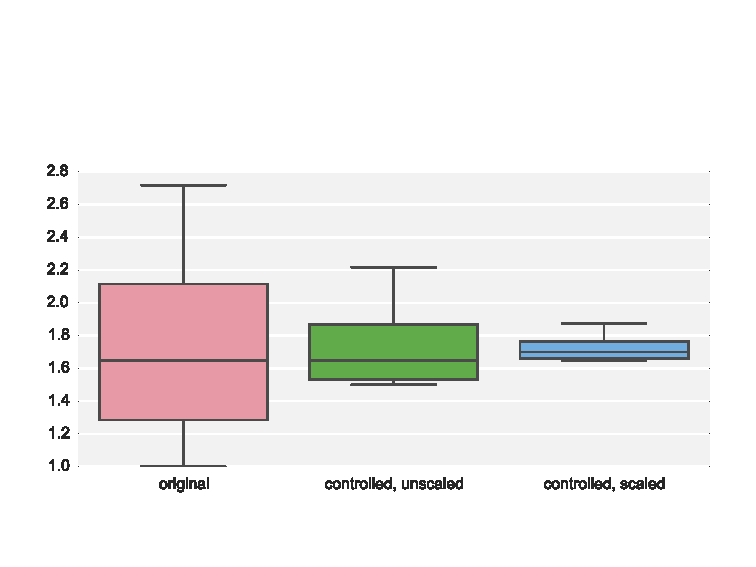
\includegraphics[width=0.7\textwidth]{control-variate.pdf}
\end{figure}



%BACKMATTER SEE DOCUMENTATION
\backmatter  % references, restarts sample


\end{document}
